\documentclass[journal]{IEEEtran}
\usepackage{fontspec}
% Times clone loaded by file name; tectonic compiles with XeTeX.
\setmainfont{texgyretermes}[Extension=.otf, UprightFont=*-regular, BoldFont=*-bold,
  ItalicFont=*-italic, BoldItalicFont=*-bolditalic]
\usepackage[shorthands=off,turkish]{babel}
\usepackage{graphicx}
\usepackage{booktabs}
\usepackage{amsmath}
\usepackage{url}
\usepackage{cite}
\usepackage{tikz}
\usetikzlibrary{positioning,arrows.meta,babel}
\graphicspath{{../../figures/}}

% Every number in the text comes from results/ through this file (written by `src.cli report`).
% Written by `python -m src.cli report`. Do not edit by hand.
\newcommand{\NSources}{203}
\newcommand{\NHumanChunks}{406}
\newcommand{\MaxChunks}{3}
\newcommand{\SingleShare}{20\%}
\newcommand{\NBlocked}{6}
\newcommand{\NTexts}{2425}
\newcommand{\NYearMin}{2015}
\newcommand{\NYearMax}{2022}
\newcommand{\NCoverD}{61\%}
\newcommand{\NCoverE}{75\%}
\newcommand{\MedWordsHuman}{302}
\newcommand{\MedMtldHuman}{84}
\newcommand{\MedWordsA}{163}
\newcommand{\MedMtldA}{90}
\newcommand{\MedWordsB}{147}
\newcommand{\MedMtldB}{121}
\newcommand{\MedWordsC}{214}
\newcommand{\MedMtldC}{132}
\newcommand{\MedWordsD}{306}
\newcommand{\MedMtldD}{199}
\newcommand{\MedWordsE}{300}
\newcommand{\MedMtldE}{169}
\newcommand{\NLargeEffects}{61}
\newcommand{\NTests}{160}
\newcommand{\HapaxDeltaMin}{0.603}
\newcommand{\HapaxDeltaMax}{0.932}
\newcommand{\FoneInLexLR}{0.997}
\newcommand{\AucInLexLR}{1.000}
\newcommand{\FoneCrossLexLR}{0.966}
\newcommand{\AucCrossLexLR}{1.000}
\newcommand{\FoneDLexLR}{0.336}
\newcommand{\AucDLexLR}{0.976}
\newcommand{\FoneELexLR}{0.960}
\newcommand{\AucELexLR}{1.000}
\newcommand{\FoneInLexSVM}{0.998}
\newcommand{\AucInLexSVM}{1.000}
\newcommand{\FoneCrossLexSVM}{0.975}
\newcommand{\AucCrossLexSVM}{1.000}
\newcommand{\FoneDLexSVM}{0.351}
\newcommand{\AucDLexSVM}{0.982}
\newcommand{\FoneELexSVM}{0.969}
\newcommand{\AucELexSVM}{1.000}
\newcommand{\FoneInStylo}{0.935}
\newcommand{\AucInStylo}{0.983}
\newcommand{\FoneCrossStylo}{0.869}
\newcommand{\AucCrossStylo}{0.956}
\newcommand{\FoneDStylo}{0.704}
\newcommand{\AucDStylo}{0.875}
\newcommand{\FoneEStylo}{0.784}
\newcommand{\AucEStylo}{0.926}
\newcommand{\FoneInTrans}{0.991}
\newcommand{\AucInTrans}{0.999}
\newcommand{\FoneCrossTrans}{0.989}
\newcommand{\AucCrossTrans}{0.999}
\newcommand{\FoneDTrans}{0.845}
\newcommand{\AucDTrans}{0.984}
\newcommand{\FoneETrans}{0.988}
\newcommand{\AucETrans}{0.999}
\newcommand{\FoneInJudge}{0.504}
\newcommand{\AucInJudge}{0.409}
\newcommand{\FoneCrossJudge}{0.504}
\newcommand{\AucCrossJudge}{0.409}
\newcommand{\FoneDJudge}{0.499}
\newcommand{\AucDJudge}{0.533}
\newcommand{\FoneEJudge}{0.628}
\newcommand{\AucEJudge}{0.754}
\newcommand{\FoneInFast}{0.748}
\newcommand{\AucInFast}{0.828}
\newcommand{\FoneCrossFast}{0.729}
\newcommand{\AucCrossFast}{0.828}
\newcommand{\FoneDFast}{0.566}
\newcommand{\AucDFast}{0.699}
\newcommand{\FoneEFast}{0.457}
\newcommand{\AucEFast}{0.613}
\newcommand{\FoneInBino}{0.815}
\newcommand{\AucInBino}{0.900}
\newcommand{\FoneCrossBino}{0.804}
\newcommand{\AucCrossBino}{0.900}
\newcommand{\FoneDBino}{0.390}
\newcommand{\AucDBino}{0.734}
\newcommand{\FoneEBino}{0.330}
\newcommand{\AucEBino}{0.671}
\newcommand{\FoneInCoord}{0.996}
\newcommand{\AucInCoord}{1.000}
\newcommand{\FoneCrossCoord}{0.993}
\newcommand{\AucCrossCoord}{1.000}
\newcommand{\FoneDCoord}{0.732}
\newcommand{\AucDCoord}{0.988}
\newcommand{\FoneECoord}{0.993}
\newcommand{\AucECoord}{1.000}
\newcommand{\PoolDLexLR}{0.888}
\newcommand{\LooLexLR}{0.998}
\newcommand{\PoolDLexSVM}{0.557}
\newcommand{\LooLexSVM}{0.995}
\newcommand{\PoolDStylo}{0.878}
\newcommand{\LooStylo}{0.899}
\newcommand{\PoolDTrans}{0.947}
\newcommand{\LooTrans}{0.975}
\newcommand{\PoolDJudge}{0.499}
\newcommand{\LooJudge}{0.504}
\newcommand{\PoolDFast}{0.590}
\newcommand{\LooFast}{0.729}
\newcommand{\PoolDBino}{0.421}
\newcommand{\LooBino}{0.805}
\newcommand{\PoolDCoord}{0.922}
\newcommand{\LooCoord}{0.994}
\newcommand{\CoordNoTransD}{0.469}
\newcommand{\CoordDropMaxOther}{0.043}
\newcommand{\HoneSigCross}{35}
\newcommand{\HoneNCross}{126}
\newcommand{\HoneDiffCross}{0.022}
\newcommand{\HoneSigExt}{85}
\newcommand{\HoneNExt}{126}
\newcommand{\HoneDiffExt}{0.254}
\newcommand{\HpDBino}{0.425}
\newcommand{\HpLoDBino}{0.386}
\newcommand{\HpHiDBino}{0.467}
\newcommand{\HpEBino}{0.485}
\newcommand{\HpLoEBino}{0.448}
\newcommand{\HpHiEBino}{0.528}
\newcommand{\HpCrossBino}{0.011}
\newcommand{\HpLoCrossBino}{-0.006}
\newcommand{\HpHiCrossBino}{0.029}
\newcommand{\HpDCoord}{0.264}
\newcommand{\HpLoDCoord}{0.235}
\newcommand{\HpHiDCoord}{0.297}
\newcommand{\HpECoord}{0.004}
\newcommand{\HpLoECoord}{-0.000}
\newcommand{\HpHiECoord}{0.008}
\newcommand{\HpCrossCoord}{0.004}
\newcommand{\HpLoCrossCoord}{0.001}
\newcommand{\HpHiCrossCoord}{0.007}
\newcommand{\HpDFast}{0.182}
\newcommand{\HpLoDFast}{0.151}
\newcommand{\HpHiDFast}{0.218}
\newcommand{\HpEFast}{0.291}
\newcommand{\HpLoEFast}{0.257}
\newcommand{\HpHiEFast}{0.331}
\newcommand{\HpCrossFast}{0.020}
\newcommand{\HpLoCrossFast}{0.003}
\newcommand{\HpHiCrossFast}{0.036}
\newcommand{\HpDLexLR}{0.660}
\newcommand{\HpLoDLexLR}{0.625}
\newcommand{\HpHiDLexLR}{0.699}
\newcommand{\HpELexLR}{0.037}
\newcommand{\HpLoELexLR}{0.026}
\newcommand{\HpHiELexLR}{0.048}
\newcommand{\HpCrossLexLR}{0.031}
\newcommand{\HpLoCrossLexLR}{0.023}
\newcommand{\HpHiCrossLexLR}{0.039}
\newcommand{\HpDLexSVM}{0.647}
\newcommand{\HpLoDLexSVM}{0.609}
\newcommand{\HpHiDLexSVM}{0.688}
\newcommand{\HpELexSVM}{0.028}
\newcommand{\HpLoELexSVM}{0.019}
\newcommand{\HpHiELexSVM}{0.039}
\newcommand{\HpCrossLexSVM}{0.023}
\newcommand{\HpLoCrossLexSVM}{0.018}
\newcommand{\HpHiCrossLexSVM}{0.029}
\newcommand{\HpDJudge}{0.005}
\newcommand{\HpLoDJudge}{-0.022}
\newcommand{\HpHiDJudge}{0.031}
\newcommand{\HpEJudge}{-0.124}
\newcommand{\HpLoEJudge}{-0.148}
\newcommand{\HpHiEJudge}{-0.103}
\newcommand{\HpCrossJudge}{0.000}
\newcommand{\HpLoCrossJudge}{-0.019}
\newcommand{\HpHiCrossJudge}{0.018}
\newcommand{\HpDStylo}{0.231}
\newcommand{\HpLoDStylo}{0.203}
\newcommand{\HpHiDStylo}{0.260}
\newcommand{\HpEStylo}{0.151}
\newcommand{\HpLoEStylo}{0.127}
\newcommand{\HpHiEStylo}{0.177}
\newcommand{\HpCrossStylo}{0.066}
\newcommand{\HpLoCrossStylo}{0.054}
\newcommand{\HpHiCrossStylo}{0.079}
\newcommand{\HpDTrans}{0.146}
\newcommand{\HpLoDTrans}{0.123}
\newcommand{\HpHiDTrans}{0.170}
\newcommand{\HpETrans}{0.003}
\newcommand{\HpLoETrans}{-0.001}
\newcommand{\HpHiETrans}{0.007}
\newcommand{\HpCrossTrans}{0.002}
\newcommand{\HpLoCrossTrans}{-0.000}
\newcommand{\HpHiCrossTrans}{0.005}
\newcommand{\HpSigCross}{3}
\newcommand{\HpNCross}{7}
\newcommand{\HpSigD}{7}
\newcommand{\HpND}{7}
\newcommand{\HpSigE}{5}
\newcommand{\HpNE}{7}
\newcommand{\FoneDLoBino}{0.349}
\newcommand{\FoneDHiBino}{0.424}
\newcommand{\FoneDLoCoord}{0.700}
\newcommand{\FoneDHiCoord}{0.762}
\newcommand{\FoneDLoFast}{0.530}
\newcommand{\FoneDHiFast}{0.595}
\newcommand{\FoneDLoLexLR}{0.295}
\newcommand{\FoneDHiLexLR}{0.374}
\newcommand{\FoneDLoLexSVM}{0.312}
\newcommand{\FoneDHiLexSVM}{0.388}
\newcommand{\FoneDLoJudge}{0.475}
\newcommand{\FoneDHiJudge}{0.519}
\newcommand{\FoneDLoStylo}{0.677}
\newcommand{\FoneDHiStylo}{0.730}
\newcommand{\FoneDLoTrans}{0.820}
\newcommand{\FoneDHiTrans}{0.868}
\newcommand{\McCoordLexSig}{16}
\newcommand{\McCoordLexN}{105}
\newcommand{\McTransLexSig}{16}
\newcommand{\McTransLexN}{105}
\newcommand{\McCoordTransSig}{3}
\newcommand{\McCoordTransN}{105}
\newcommand{\JudgeHumanFlag}{82\%}
\newcommand{\PoolTwoDLexLR}{0.767}
\newcommand{\PoolTwoDLexSVM}{0.456}
\newcommand{\PoolTwoDStylo}{0.815}
\newcommand{\PoolTwoDTrans}{0.952}
\newcommand{\PoolTwoDJudge}{0.499}
\newcommand{\PoolTwoDFast}{0.586}
\newcommand{\PoolTwoDBino}{0.412}
\newcommand{\PoolTwoDCoord}{0.888}
\newcommand{\CmATP}{74}
\newcommand{\CmAFP}{2}
\newcommand{\CmAFN}{0}
\newcommand{\CmATN}{72}
\newcommand{\CmDTP}{30}
\newcommand{\CmDFP}{2}
\newcommand{\CmDFN}{44}
\newcommand{\CmDTN}{72}
\newcommand{\AblTfidfIn}{0.997}
\newcommand{\AblTfidfCross}{0.966}
\newcommand{\AblTfidfD}{0.336}
\newcommand{\AblStylometryIn}{0.935}
\newcommand{\AblStylometryCross}{0.869}
\newcommand{\AblStylometryD}{0.704}
\newcommand{\AblBothIn}{0.966}
\newcommand{\AblBothCross}{0.921}
\newcommand{\AblBothD}{0.730}
\newcommand{\AblLrNoCleanIn}{0.997}
\newcommand{\AblLrNoCleanCross}{0.965}
\newcommand{\AblLrNoCleanD}{0.342}
\newcommand{\AblLrMaskedIn}{0.996}
\newcommand{\AblLrMaskedCross}{0.968}
\newcommand{\AblLrMaskedD}{0.346}
\newcommand{\AblTransformerMaskedIn}{0.987}
\newcommand{\AblTransformerMaskedCross}{0.985}
\newcommand{\AblTransformerMaskedD}{0.882}
\newcommand{\AblGroupLengthIn}{0.871}
\newcommand{\AblGroupLengthCross}{0.792}
\newcommand{\AblGroupLengthD}{0.504}
\newcommand{\AblGroupLexicalIn}{0.842}
\newcommand{\AblGroupLexicalCross}{0.815}
\newcommand{\AblGroupLexicalD}{0.865}
\newcommand{\AblGroupPunctuationIn}{0.820}
\newcommand{\AblGroupPunctuationCross}{0.767}
\newcommand{\AblGroupPunctuationD}{0.487}
\newcommand{\AblGroupRepetitionIn}{0.795}
\newcommand{\AblGroupRepetitionCross}{0.770}
\newcommand{\AblGroupRepetitionD}{0.818}
\newcommand{\AblGroupPosIn}{0.801}
\newcommand{\AblGroupPosCross}{0.748}
\newcommand{\AblGroupPosD}{0.768}
\newcommand{\SingleInLexLR}{0.498}
\newcommand{\SingleCrossLexLR}{0.254}
\newcommand{\SingleInStylo}{0.679}
\newcommand{\SingleCrossStylo}{0.529}
\newcommand{\TplRecallMin}{0.817}
\newcommand{\TplRecallMax}{1.000}
\newcommand{\TplAucMin}{1.000}
\newcommand{\LenAN}{2}
\newcommand{\LenALexLR}{1.000}
\newcommand{\LenAAucLexLR}{1.000}
\newcommand{\SameALexLR}{0.994}
\newcommand{\LenALexSVM}{1.000}
\newcommand{\LenAAucLexSVM}{1.000}
\newcommand{\SameALexSVM}{0.996}
\newcommand{\LenAStylo}{0.250}
\newcommand{\LenAAucStylo}{0.875}
\newcommand{\SameAStylo}{0.937}
\newcommand{\LenATrans}{1.000}
\newcommand{\LenAAucTrans}{1.000}
\newcommand{\SameATrans}{0.988}
\newcommand{\LenAJudge}{0.733}
\newcommand{\LenAAucJudge}{0.625}
\newcommand{\SameAJudge}{0.494}
\newcommand{\LenAFast}{0.833}
\newcommand{\LenAAucFast}{0.875}
\newcommand{\SameAFast}{0.809}
\newcommand{\LenABino}{0.833}
\newcommand{\LenAAucBino}{0.875}
\newcommand{\SameABino}{0.881}
\newcommand{\LenACoord}{1.000}
\newcommand{\LenAAucCoord}{1.000}
\newcommand{\SameACoord}{0.993}
\newcommand{\LenBN}{12}
\newcommand{\LenBLexLR}{1.000}
\newcommand{\LenBAucLexLR}{1.000}
\newcommand{\SameBLexLR}{0.998}
\newcommand{\LenBLexSVM}{1.000}
\newcommand{\LenBAucLexSVM}{1.000}
\newcommand{\SameBLexSVM}{1.000}
\newcommand{\LenBStylo}{0.764}
\newcommand{\LenBAucStylo}{0.949}
\newcommand{\SameBStylo}{0.924}
\newcommand{\LenBTrans}{0.988}
\newcommand{\LenBAucTrans}{1.000}
\newcommand{\SameBTrans}{0.990}
\newcommand{\LenBJudge}{0.667}
\newcommand{\LenBAucJudge}{0.675}
\newcommand{\SameBJudge}{0.428}
\newcommand{\LenBFast}{0.799}
\newcommand{\LenBAucFast}{0.991}
\newcommand{\SameBFast}{0.709}
\newcommand{\LenBBino}{0.893}
\newcommand{\LenBAucBino}{1.000}
\newcommand{\SameBBino}{0.743}
\newcommand{\LenBCoord}{1.000}
\newcommand{\LenBAucCoord}{1.000}
\newcommand{\SameBCoord}{0.996}
\newcommand{\LenCN}{23}
\newcommand{\LenCLexLR}{1.000}
\newcommand{\LenCAucLexLR}{1.000}
\newcommand{\SameCLexLR}{0.998}
\newcommand{\LenCLexSVM}{1.000}
\newcommand{\LenCAucLexSVM}{1.000}
\newcommand{\SameCLexSVM}{0.998}
\newcommand{\LenCStylo}{0.926}
\newcommand{\LenCAucStylo}{0.986}
\newcommand{\SameCStylo}{0.945}
\newcommand{\LenCTrans}{1.000}
\newcommand{\LenCAucTrans}{1.000}
\newcommand{\SameCTrans}{0.996}
\newcommand{\LenCJudge}{0.635}
\newcommand{\LenCAucJudge}{0.499}
\newcommand{\SameCJudge}{0.589}
\newcommand{\LenCFast}{0.763}
\newcommand{\LenCAucFast}{0.835}
\newcommand{\SameCFast}{0.727}
\newcommand{\LenCBino}{0.843}
\newcommand{\LenCAucBino}{0.931}
\newcommand{\SameCBino}{0.821}
\newcommand{\LenCCoord}{1.000}
\newcommand{\LenCAucCoord}{1.000}
\newcommand{\SameCCoord}{1.000}
\newcommand{\TopicCrossApt}{0.981}
\newcommand{\TopicCrossMalware}{1.000}
\newcommand{\TopicCrossOther}{1.000}
\newcommand{\TopicCrossPhishing}{0.982}
\newcommand{\TopicCrossRansomware}{0.990}
\newcommand{\TopicCrossVulnerability}{0.993}
\newcommand{\TopicCrossMin}{0.981}
\newcommand{\TopicCrossMax}{1.000}
\newcommand{\TopicDApt}{0.544}
\newcommand{\TopicDMalware}{0.574}
\newcommand{\TopicDOther}{0.889}
\newcommand{\TopicDPhishing}{0.727}
\newcommand{\TopicDRansomware}{0.615}
\newcommand{\TopicDVulnerability}{0.564}
\newcommand{\TopicDMin}{0.544}
\newcommand{\TopicDMax}{0.889}
\newcommand{\TopFeature}{n\_words}
\newcommand{\NVarTexts}{6293}
\newcommand{\NVarChunks}{191}
\newcommand{\NExtSourcesMicrosoft}{80}
\newcommand{\NExtChunksMicrosoft}{231}
\newcommand{\ExtFirstMicrosoft}{2012-01-16}
\newcommand{\ExtLastMicrosoft}{2022-11-22}
\newcommand{\ExtWordsMicrosoft}{319}
\newcommand{\NExtSourcesMandiant}{80}
\newcommand{\NExtChunksMandiant}{207}
\newcommand{\ExtFirstMandiant}{2010-08-16}
\newcommand{\ExtLastMandiant}{2022-11-28}
\newcommand{\ExtWordsMandiant}{306}
\newcommand{\NPubLarge}{11}
\newcommand{\NPubTests}{64}
\newcommand{\PubMicrosoftNWordsDelta}{0.311}
\newcommand{\PubMicrosoftMtldDelta}{0.249}
\newcommand{\PubMicrosoftPosPropnDelta}{-0.595}
\newcommand{\PubMicrosoftPosPronDelta}{0.785}
\newcommand{\PubMandiantNWordsDelta}{0.076}
\newcommand{\PubMandiantMtldDelta}{0.160}
\newcommand{\PubMandiantPosPropnDelta}{-0.430}
\newcommand{\PubMandiantPosPronDelta}{0.648}
\newcommand{\PubCisaLexlrFpr}{0.014}
\newcommand{\PubCisaLexlrRec}{0.999}
\newcommand{\PubCisaLexlrFone}{0.993}
\newcommand{\PubCisaLexlrAuc}{1.000}
\newcommand{\PubCisaTransFpr}{0.055}
\newcommand{\PubCisaTransRec}{1.000}
\newcommand{\PubCisaTransFone}{0.973}
\newcommand{\PubCisaTransAuc}{1.000}
\newcommand{\PubCisaCoordFpr}{0.005}
\newcommand{\PubCisaCoordRec}{1.000}
\newcommand{\PubCisaCoordFone}{0.998}
\newcommand{\PubCisaCoordAuc}{1.000}
\newcommand{\PubCisaFastFpr}{0.260}
\newcommand{\PubCisaFastRec}{0.743}
\newcommand{\PubCisaFastFone}{0.740}
\newcommand{\PubCisaFastAuc}{0.828}
\newcommand{\PubCisaBinoFpr}{0.106}
\newcommand{\PubCisaBinoRec}{0.760}
\newcommand{\PubCisaBinoFone}{0.812}
\newcommand{\PubCisaBinoAuc}{0.900}
\newcommand{\PubMicrosoftLexlrFpr}{0.154}
\newcommand{\PubMicrosoftLexlrRec}{1.000}
\newcommand{\PubMicrosoftLexlrFone}{0.929}
\newcommand{\PubMicrosoftLexlrAuc}{1.000}
\newcommand{\PubMicrosoftLexlrFprAug}{0.016}
\newcommand{\PubMicrosoftTransFpr}{0.205}
\newcommand{\PubMicrosoftTransRec}{1.000}
\newcommand{\PubMicrosoftTransFone}{0.909}
\newcommand{\PubMicrosoftTransAuc}{1.000}
\newcommand{\PubMicrosoftTransFprAug}{0.049}
\newcommand{\PubMicrosoftCoordFpr}{0.045}
\newcommand{\PubMicrosoftCoordRec}{1.000}
\newcommand{\PubMicrosoftCoordFone}{0.978}
\newcommand{\PubMicrosoftCoordAuc}{1.000}
\newcommand{\PubMicrosoftCoordFprAug}{0.003}
\newcommand{\PubMicrosoftFastFpr}{0.124}
\newcommand{\PubMicrosoftFastRec}{0.895}
\newcommand{\PubMicrosoftFastFone}{0.886}
\newcommand{\PubMicrosoftFastAuc}{0.954}
\newcommand{\PubMicrosoftBinoFpr}{0.033}
\newcommand{\PubMicrosoftBinoRec}{0.892}
\newcommand{\PubMicrosoftBinoFone}{0.926}
\newcommand{\PubMicrosoftBinoAuc}{0.979}
\newcommand{\PubMandiantLexlrFpr}{0.143}
\newcommand{\PubMandiantLexlrRec}{1.000}
\newcommand{\PubMandiantLexlrFone}{0.933}
\newcommand{\PubMandiantLexlrAuc}{1.000}
\newcommand{\PubMandiantLexlrFprAug}{0.013}
\newcommand{\PubMandiantTransFpr}{0.225}
\newcommand{\PubMandiantTransRec}{1.000}
\newcommand{\PubMandiantTransFone}{0.901}
\newcommand{\PubMandiantTransAuc}{1.000}
\newcommand{\PubMandiantTransFprAug}{0.045}
\newcommand{\PubMandiantCoordFpr}{0.063}
\newcommand{\PubMandiantCoordRec}{1.000}
\newcommand{\PubMandiantCoordFone}{0.970}
\newcommand{\PubMandiantCoordAuc}{1.000}
\newcommand{\PubMandiantCoordFprAug}{0.018}
\newcommand{\PubMandiantFastFpr}{0.126}
\newcommand{\PubMandiantFastRec}{0.846}
\newcommand{\PubMandiantFastFone}{0.857}
\newcommand{\PubMandiantFastAuc}{0.940}
\newcommand{\PubMandiantBinoFpr}{0.016}
\newcommand{\PubMandiantBinoRec}{0.836}
\newcommand{\PubMandiantBinoFone}{0.901}
\newcommand{\PubMandiantBinoAuc}{0.977}
\newcommand{\CalLexlrRawInBrier}{0.036}
\newcommand{\CalLexlrRawInEce}{0.170}
\newcommand{\CalLexlrRawInNll}{0.194}
\newcommand{\CalLexlrRawDBrier}{0.201}
\newcommand{\CalLexlrRawDEce}{0.311}
\newcommand{\CalLexlrRawDNll}{0.571}
\newcommand{\CalLexlrRawEBrier}{0.074}
\newcommand{\CalLexlrRawEEce}{0.245}
\newcommand{\CalLexlrRawENll}{0.296}
\newcommand{\CalLexlrPlattInBrier}{0.002}
\newcommand{\CalLexlrPlattInEce}{0.004}
\newcommand{\CalLexlrPlattInNll}{0.014}
\newcommand{\CalLexlrPlattDBrier}{0.269}
\newcommand{\CalLexlrPlattDEce}{0.297}
\newcommand{\CalLexlrPlattDNll}{1.822}
\newcommand{\CalLexlrPlattEBrier}{0.015}
\newcommand{\CalLexlrPlattEEce}{0.027}
\newcommand{\CalLexlrPlattENll}{0.056}
\newcommand{\CalLexlrTemperatureInBrier}{0.003}
\newcommand{\CalLexlrTemperatureInEce}{0.008}
\newcommand{\CalLexlrTemperatureInNll}{0.027}
\newcommand{\CalLexlrTemperatureDBrier}{0.348}
\newcommand{\CalLexlrTemperatureDEce}{0.377}
\newcommand{\CalLexlrTemperatureDNll}{2.892}
\newcommand{\CalLexlrTemperatureEBrier}{0.030}
\newcommand{\CalLexlrTemperatureEEce}{0.051}
\newcommand{\CalLexlrTemperatureENll}{0.139}
\newcommand{\CalLexlrIsotonicInBrier}{0.003}
\newcommand{\CalLexlrIsotonicInEce}{0.007}
\newcommand{\CalLexlrIsotonicInNll}{0.018}
\newcommand{\CalLexlrIsotonicDBrier}{0.241}
\newcommand{\CalLexlrIsotonicDEce}{0.287}
\newcommand{\CalLexlrIsotonicDNll}{2.050}
\newcommand{\CalLexlrIsotonicEBrier}{0.015}
\newcommand{\CalLexlrIsotonicEEce}{0.036}
\newcommand{\CalLexlrIsotonicENll}{0.058}
\newcommand{\CalTransRawInBrier}{0.007}
\newcommand{\CalTransRawInEce}{0.015}
\newcommand{\CalTransRawInNll}{0.032}
\newcommand{\CalTransRawDBrier}{0.104}
\newcommand{\CalTransRawDEce}{0.120}
\newcommand{\CalTransRawDNll}{0.406}
\newcommand{\CalTransRawEBrier}{0.010}
\newcommand{\CalTransRawEEce}{0.018}
\newcommand{\CalTransRawENll}{0.039}
\newcommand{\CalTransPlattInBrier}{0.007}
\newcommand{\CalTransPlattInEce}{0.010}
\newcommand{\CalTransPlattInNll}{0.037}
\newcommand{\CalTransPlattDBrier}{0.178}
\newcommand{\CalTransPlattDEce}{0.190}
\newcommand{\CalTransPlattDNll}{1.755}
\newcommand{\CalTransPlattEBrier}{0.019}
\newcommand{\CalTransPlattEEce}{0.024}
\newcommand{\CalTransPlattENll}{0.128}
\newcommand{\CalTransTemperatureInBrier}{0.008}
\newcommand{\CalTransTemperatureInEce}{0.013}
\newcommand{\CalTransTemperatureInNll}{0.044}
\newcommand{\CalTransTemperatureDBrier}{0.111}
\newcommand{\CalTransTemperatureDEce}{0.122}
\newcommand{\CalTransTemperatureDNll}{0.832}
\newcommand{\CalTransTemperatureEBrier}{0.010}
\newcommand{\CalTransTemperatureEEce}{0.018}
\newcommand{\CalTransTemperatureENll}{0.062}
\newcommand{\CalTransIsotonicInBrier}{0.006}
\newcommand{\CalTransIsotonicInEce}{0.008}
\newcommand{\CalTransIsotonicInNll}{0.042}
\newcommand{\CalTransIsotonicDBrier}{0.168}
\newcommand{\CalTransIsotonicDEce}{0.192}
\newcommand{\CalTransIsotonicDNll}{1.746}
\newcommand{\CalTransIsotonicEBrier}{0.016}
\newcommand{\CalTransIsotonicEEce}{0.022}
\newcommand{\CalTransIsotonicENll}{0.131}
\newcommand{\CalCoordRawInBrier}{0.002}
\newcommand{\CalCoordRawInEce}{0.006}
\newcommand{\CalCoordRawInNll}{0.009}
\newcommand{\CalCoordRawDBrier}{0.161}
\newcommand{\CalCoordRawDEce}{0.209}
\newcommand{\CalCoordRawDNll}{0.594}
\newcommand{\CalCoordRawEBrier}{0.007}
\newcommand{\CalCoordRawEEce}{0.023}
\newcommand{\CalCoordRawENll}{0.031}
\newcommand{\CalCoordPlattInBrier}{0.003}
\newcommand{\CalCoordPlattInEce}{0.005}
\newcommand{\CalCoordPlattInNll}{0.023}
\newcommand{\CalCoordPlattDBrier}{0.180}
\newcommand{\CalCoordPlattDEce}{0.202}
\newcommand{\CalCoordPlattDNll}{1.374}
\newcommand{\CalCoordPlattEBrier}{0.007}
\newcommand{\CalCoordPlattEEce}{0.013}
\newcommand{\CalCoordPlattENll}{0.035}
\newcommand{\CalCoordTemperatureInBrier}{0.004}
\newcommand{\CalCoordTemperatureInEce}{0.005}
\newcommand{\CalCoordTemperatureInNll}{0.033}
\newcommand{\CalCoordTemperatureDBrier}{0.191}
\newcommand{\CalCoordTemperatureDEce}{0.203}
\newcommand{\CalCoordTemperatureDNll}{2.124}
\newcommand{\CalCoordTemperatureEBrier}{0.008}
\newcommand{\CalCoordTemperatureEEce}{0.013}
\newcommand{\CalCoordTemperatureENll}{0.059}
\newcommand{\CalCoordIsotonicInBrier}{0.003}
\newcommand{\CalCoordIsotonicInEce}{0.006}
\newcommand{\CalCoordIsotonicInNll}{0.026}
\newcommand{\CalCoordIsotonicDBrier}{0.172}
\newcommand{\CalCoordIsotonicDEce}{0.206}
\newcommand{\CalCoordIsotonicDNll}{1.450}
\newcommand{\CalCoordIsotonicEBrier}{0.007}
\newcommand{\CalCoordIsotonicEEce}{0.015}
\newcommand{\CalCoordIsotonicENll}{0.038}
\newcommand{\ThrInLexlrFixedFOne}{0.997}
\newcommand{\ThrInLexlrFixedRecall}{0.993}
\newcommand{\ThrInLexlrFixedFpr}{0.000}
\newcommand{\ThrInLexlrFixedPrecision}{1.000}
\newcommand{\ThrCrossLexlrFixedFOne}{0.966}
\newcommand{\ThrCrossLexlrFixedRecall}{0.937}
\newcommand{\ThrCrossLexlrFixedFpr}{0.000}
\newcommand{\ThrCrossLexlrFixedPrecision}{1.000}
\newcommand{\ThrDLexlrFixedFOne}{0.336}
\newcommand{\ThrDLexlrFixedRecall}{0.213}
\newcommand{\ThrDLexlrFixedFpr}{0.000}
\newcommand{\ThrDLexlrFixedPrecision}{1.000}
\newcommand{\ThrELexlrFixedFOne}{0.960}
\newcommand{\ThrELexlrFixedRecall}{0.925}
\newcommand{\ThrELexlrFixedFpr}{0.000}
\newcommand{\ThrELexlrFixedPrecision}{1.000}
\newcommand{\ThrExternalLexlrFixedFOne}{0.982}
\newcommand{\ThrExternalLexlrFixedRecall}{0.970}
\newcommand{\ThrExternalLexlrFixedFpr}{0.004}
\newcommand{\ThrExternalLexlrFixedPrecision}{0.996}
\newcommand{\ThrInLexlrValfFOne}{0.997}
\newcommand{\ThrInLexlrValfRecall}{0.994}
\newcommand{\ThrInLexlrValfFpr}{0.000}
\newcommand{\ThrInLexlrValfPrecision}{1.000}
\newcommand{\ThrCrossLexlrValfFOne}{0.977}
\newcommand{\ThrCrossLexlrValfRecall}{0.958}
\newcommand{\ThrCrossLexlrValfFpr}{0.000}
\newcommand{\ThrCrossLexlrValfPrecision}{1.000}
\newcommand{\ThrDLexlrValfFOne}{0.510}
\newcommand{\ThrDLexlrValfRecall}{0.373}
\newcommand{\ThrDLexlrValfFpr}{0.000}
\newcommand{\ThrDLexlrValfPrecision}{1.000}
\newcommand{\ThrELexlrValfFOne}{0.980}
\newcommand{\ThrELexlrValfRecall}{0.964}
\newcommand{\ThrELexlrValfFpr}{0.000}
\newcommand{\ThrELexlrValfPrecision}{1.000}
\newcommand{\ThrExternalLexlrValfFOne}{0.982}
\newcommand{\ThrExternalLexlrValfRecall}{0.981}
\newcommand{\ThrExternalLexlrValfFpr}{0.017}
\newcommand{\ThrExternalLexlrValfPrecision}{0.984}
\newcommand{\ThrInLexlrPseudoFOne}{0.996}
\newcommand{\ThrInLexlrPseudoRecall}{0.997}
\newcommand{\ThrInLexlrPseudoFpr}{0.006}
\newcommand{\ThrInLexlrPseudoPrecision}{0.994}
\newcommand{\ThrCrossLexlrPseudoFOne}{0.994}
\newcommand{\ThrCrossLexlrPseudoRecall}{0.991}
\newcommand{\ThrCrossLexlrPseudoFpr}{0.004}
\newcommand{\ThrCrossLexlrPseudoPrecision}{0.996}
\newcommand{\ThrDLexlrPseudoFOne}{0.752}
\newcommand{\ThrDLexlrPseudoRecall}{0.613}
\newcommand{\ThrDLexlrPseudoFpr}{0.006}
\newcommand{\ThrDLexlrPseudoPrecision}{0.991}
\newcommand{\ThrELexlrPseudoFOne}{0.996}
\newcommand{\ThrELexlrPseudoRecall}{0.997}
\newcommand{\ThrELexlrPseudoFpr}{0.006}
\newcommand{\ThrELexlrPseudoPrecision}{0.994}
\newcommand{\ThrExternalLexlrPseudoFOne}{0.973}
\newcommand{\ThrExternalLexlrPseudoRecall}{0.995}
\newcommand{\ThrExternalLexlrPseudoFpr}{0.054}
\newcommand{\ThrExternalLexlrPseudoPrecision}{0.952}
\newcommand{\ThrInLexlrHumfiveFOne}{0.986}
\newcommand{\ThrInLexlrHumfiveRecall}{0.999}
\newcommand{\ThrInLexlrHumfiveFpr}{0.028}
\newcommand{\ThrInLexlrHumfivePrecision}{0.974}
\newcommand{\ThrCrossLexlrHumfiveFOne}{0.985}
\newcommand{\ThrCrossLexlrHumfiveRecall}{0.998}
\newcommand{\ThrCrossLexlrHumfiveFpr}{0.028}
\newcommand{\ThrCrossLexlrHumfivePrecision}{0.974}
\newcommand{\ThrDLexlrHumfiveFOne}{0.869}
\newcommand{\ThrDLexlrHumfiveRecall}{0.797}
\newcommand{\ThrDLexlrHumfiveFpr}{0.028}
\newcommand{\ThrDLexlrHumfivePrecision}{0.970}
\newcommand{\ThrELexlrHumfiveFOne}{0.986}
\newcommand{\ThrELexlrHumfiveRecall}{1.000}
\newcommand{\ThrELexlrHumfiveFpr}{0.028}
\newcommand{\ThrELexlrHumfivePrecision}{0.974}
\newcommand{\ThrExternalLexlrHumfiveFOne}{0.914}
\newcommand{\ThrExternalLexlrHumfiveRecall}{0.999}
\newcommand{\ThrExternalLexlrHumfiveFpr}{0.189}
\newcommand{\ThrExternalLexlrHumfivePrecision}{0.844}
\newcommand{\ThrInLexlrHumoneFOne}{0.991}
\newcommand{\ThrInLexlrHumoneRecall}{0.999}
\newcommand{\ThrInLexlrHumoneFpr}{0.017}
\newcommand{\ThrInLexlrHumonePrecision}{0.984}
\newcommand{\ThrCrossLexlrHumoneFOne}{0.991}
\newcommand{\ThrCrossLexlrHumoneRecall}{0.998}
\newcommand{\ThrCrossLexlrHumoneFpr}{0.017}
\newcommand{\ThrCrossLexlrHumonePrecision}{0.984}
\newcommand{\ThrDLexlrHumoneFOne}{0.849}
\newcommand{\ThrDLexlrHumoneRecall}{0.754}
\newcommand{\ThrDLexlrHumoneFpr}{0.017}
\newcommand{\ThrDLexlrHumonePrecision}{0.981}
\newcommand{\ThrELexlrHumoneFOne}{0.991}
\newcommand{\ThrELexlrHumoneRecall}{0.999}
\newcommand{\ThrELexlrHumoneFpr}{0.017}
\newcommand{\ThrELexlrHumonePrecision}{0.984}
\newcommand{\ThrExternalLexlrHumoneFOne}{0.936}
\newcommand{\ThrExternalLexlrHumoneRecall}{0.999}
\newcommand{\ThrExternalLexlrHumoneFpr}{0.137}
\newcommand{\ThrExternalLexlrHumonePrecision}{0.882}
\newcommand{\ThrInTransFixedFOne}{0.991}
\newcommand{\ThrInTransFixedRecall}{0.997}
\newcommand{\ThrInTransFixedFpr}{0.015}
\newcommand{\ThrInTransFixedPrecision}{0.985}
\newcommand{\ThrCrossTransFixedFOne}{0.989}
\newcommand{\ThrCrossTransFixedRecall}{0.993}
\newcommand{\ThrCrossTransFixedFpr}{0.015}
\newcommand{\ThrCrossTransFixedPrecision}{0.985}
\newcommand{\ThrDTransFixedFOne}{0.845}
\newcommand{\ThrDTransFixedRecall}{0.770}
\newcommand{\ThrDTransFixedFpr}{0.015}
\newcommand{\ThrDTransFixedPrecision}{0.981}
\newcommand{\ThrETransFixedFOne}{0.988}
\newcommand{\ThrETransFixedRecall}{0.991}
\newcommand{\ThrETransFixedFpr}{0.015}
\newcommand{\ThrETransFixedPrecision}{0.985}
\newcommand{\ThrExternalTransFixedFOne}{0.953}
\newcommand{\ThrExternalTransFixedRecall}{0.998}
\newcommand{\ThrExternalTransFixedFpr}{0.099}
\newcommand{\ThrExternalTransFixedPrecision}{0.914}
\newcommand{\ThrInTransValfFOne}{0.992}
\newcommand{\ThrInTransValfRecall}{0.994}
\newcommand{\ThrInTransValfFpr}{0.010}
\newcommand{\ThrInTransValfPrecision}{0.991}
\newcommand{\ThrCrossTransValfFOne}{0.989}
\newcommand{\ThrCrossTransValfRecall}{0.989}
\newcommand{\ThrCrossTransValfFpr}{0.010}
\newcommand{\ThrCrossTransValfPrecision}{0.991}
\newcommand{\ThrDTransValfFOne}{0.771}
\newcommand{\ThrDTransValfRecall}{0.675}
\newcommand{\ThrDTransValfFpr}{0.010}
\newcommand{\ThrDTransValfPrecision}{0.988}
\newcommand{\ThrETransValfFOne}{0.984}
\newcommand{\ThrETransValfRecall}{0.978}
\newcommand{\ThrETransValfFpr}{0.010}
\newcommand{\ThrETransValfPrecision}{0.991}
\newcommand{\ThrExternalTransValfFOne}{0.964}
\newcommand{\ThrExternalTransValfRecall}{0.995}
\newcommand{\ThrExternalTransValfFpr}{0.071}
\newcommand{\ThrExternalTransValfPrecision}{0.936}
\newcommand{\ThrInTransPseudoFOne}{0.988}
\newcommand{\ThrInTransPseudoRecall}{0.996}
\newcommand{\ThrInTransPseudoFpr}{0.021}
\newcommand{\ThrInTransPseudoPrecision}{0.980}
\newcommand{\ThrCrossTransPseudoFOne}{0.987}
\newcommand{\ThrCrossTransPseudoRecall}{0.987}
\newcommand{\ThrCrossTransPseudoFpr}{0.014}
\newcommand{\ThrCrossTransPseudoPrecision}{0.987}
\newcommand{\ThrDTransPseudoFOne}{0.801}
\newcommand{\ThrDTransPseudoRecall}{0.722}
\newcommand{\ThrDTransPseudoFpr}{0.021}
\newcommand{\ThrDTransPseudoPrecision}{0.974}
\newcommand{\ThrETransPseudoFOne}{0.980}
\newcommand{\ThrETransPseudoRecall}{0.980}
\newcommand{\ThrETransPseudoFpr}{0.021}
\newcommand{\ThrETransPseudoPrecision}{0.980}
\newcommand{\ThrExternalTransPseudoFOne}{0.965}
\newcommand{\ThrExternalTransPseudoRecall}{0.993}
\newcommand{\ThrExternalTransPseudoFpr}{0.070}
\newcommand{\ThrExternalTransPseudoPrecision}{0.940}
\newcommand{\ThrInTransHumfiveFOne}{0.975}
\newcommand{\ThrInTransHumfiveRecall}{0.999}
\newcommand{\ThrInTransHumfiveFpr}{0.049}
\newcommand{\ThrInTransHumfivePrecision}{0.954}
\newcommand{\ThrCrossTransHumfiveFOne}{0.975}
\newcommand{\ThrCrossTransHumfiveRecall}{0.998}
\newcommand{\ThrCrossTransHumfiveFpr}{0.049}
\newcommand{\ThrCrossTransHumfivePrecision}{0.954}
\newcommand{\ThrDTransHumfiveFOne}{0.939}
\newcommand{\ThrDTransHumfiveRecall}{0.929}
\newcommand{\ThrDTransHumfiveFpr}{0.049}
\newcommand{\ThrDTransHumfivePrecision}{0.951}
\newcommand{\ThrETransHumfiveFOne}{0.975}
\newcommand{\ThrETransHumfiveRecall}{0.998}
\newcommand{\ThrETransHumfiveFpr}{0.049}
\newcommand{\ThrETransHumfivePrecision}{0.954}
\newcommand{\ThrExternalTransHumfiveFOne}{0.908}
\newcommand{\ThrExternalTransHumfiveRecall}{1.000}
\newcommand{\ThrExternalTransHumfiveFpr}{0.203}
\newcommand{\ThrExternalTransHumfivePrecision}{0.833}
\newcommand{\ThrInTransHumoneFOne}{0.989}
\newcommand{\ThrInTransHumoneRecall}{0.997}
\newcommand{\ThrInTransHumoneFpr}{0.019}
\newcommand{\ThrInTransHumonePrecision}{0.981}
\newcommand{\ThrCrossTransHumoneFOne}{0.987}
\newcommand{\ThrCrossTransHumoneRecall}{0.993}
\newcommand{\ThrCrossTransHumoneFpr}{0.019}
\newcommand{\ThrCrossTransHumonePrecision}{0.981}
\newcommand{\ThrDTransHumoneFOne}{0.860}
\newcommand{\ThrDTransHumoneRecall}{0.788}
\newcommand{\ThrDTransHumoneFpr}{0.019}
\newcommand{\ThrDTransHumonePrecision}{0.976}
\newcommand{\ThrETransHumoneFOne}{0.984}
\newcommand{\ThrETransHumoneRecall}{0.987}
\newcommand{\ThrETransHumoneFpr}{0.019}
\newcommand{\ThrETransHumonePrecision}{0.981}
\newcommand{\ThrExternalTransHumoneFOne}{0.953}
\newcommand{\ThrExternalTransHumoneRecall}{0.998}
\newcommand{\ThrExternalTransHumoneFpr}{0.099}
\newcommand{\ThrExternalTransHumonePrecision}{0.912}
\newcommand{\ThrInCoordFixedFOne}{0.996}
\newcommand{\ThrInCoordFixedRecall}{0.996}
\newcommand{\ThrInCoordFixedFpr}{0.003}
\newcommand{\ThrInCoordFixedPrecision}{0.997}
\newcommand{\ThrCrossCoordFixedFOne}{0.993}
\newcommand{\ThrCrossCoordFixedRecall}{0.989}
\newcommand{\ThrCrossCoordFixedFpr}{0.003}
\newcommand{\ThrCrossCoordFixedPrecision}{0.997}
\newcommand{\ThrDCoordFixedFOne}{0.732}
\newcommand{\ThrDCoordFixedRecall}{0.605}
\newcommand{\ThrDCoordFixedFpr}{0.003}
\newcommand{\ThrDCoordFixedPrecision}{0.993}
\newcommand{\ThrECoordFixedFOne}{0.993}
\newcommand{\ThrECoordFixedRecall}{0.988}
\newcommand{\ThrECoordFixedFpr}{0.003}
\newcommand{\ThrECoordFixedPrecision}{0.997}
\newcommand{\ThrExternalCoordFixedFOne}{0.990}
\newcommand{\ThrExternalCoordFixedRecall}{0.996}
\newcommand{\ThrExternalCoordFixedFpr}{0.015}
\newcommand{\ThrExternalCoordFixedPrecision}{0.985}
\newcommand{\ThrInCoordValfFOne}{0.996}
\newcommand{\ThrInCoordValfRecall}{0.996}
\newcommand{\ThrInCoordValfFpr}{0.003}
\newcommand{\ThrInCoordValfPrecision}{0.997}
\newcommand{\ThrCrossCoordValfFOne}{0.992}
\newcommand{\ThrCrossCoordValfRecall}{0.987}
\newcommand{\ThrCrossCoordValfFpr}{0.003}
\newcommand{\ThrCrossCoordValfPrecision}{0.997}
\newcommand{\ThrDCoordValfFOne}{0.719}
\newcommand{\ThrDCoordValfRecall}{0.586}
\newcommand{\ThrDCoordValfFpr}{0.003}
\newcommand{\ThrDCoordValfPrecision}{0.994}
\newcommand{\ThrECoordValfFOne}{0.992}
\newcommand{\ThrECoordValfRecall}{0.987}
\newcommand{\ThrECoordValfFpr}{0.003}
\newcommand{\ThrECoordValfPrecision}{0.997}
\newcommand{\ThrExternalCoordValfFOne}{0.991}
\newcommand{\ThrExternalCoordValfRecall}{0.995}
\newcommand{\ThrExternalCoordValfFpr}{0.014}
\newcommand{\ThrExternalCoordValfPrecision}{0.986}
\newcommand{\ThrInCoordPseudoFOne}{0.994}
\newcommand{\ThrInCoordPseudoRecall}{0.999}
\newcommand{\ThrInCoordPseudoFpr}{0.010}
\newcommand{\ThrInCoordPseudoPrecision}{0.990}
\newcommand{\ThrCrossCoordPseudoFOne}{0.992}
\newcommand{\ThrCrossCoordPseudoRecall}{0.991}
\newcommand{\ThrCrossCoordPseudoFpr}{0.006}
\newcommand{\ThrCrossCoordPseudoPrecision}{0.994}
\newcommand{\ThrDCoordPseudoFOne}{0.807}
\newcommand{\ThrDCoordPseudoRecall}{0.713}
\newcommand{\ThrDCoordPseudoFpr}{0.010}
\newcommand{\ThrDCoordPseudoPrecision}{0.986}
\newcommand{\ThrECoordPseudoFOne}{0.990}
\newcommand{\ThrECoordPseudoRecall}{0.990}
\newcommand{\ThrECoordPseudoFpr}{0.010}
\newcommand{\ThrECoordPseudoPrecision}{0.990}
\newcommand{\ThrExternalCoordPseudoFOne}{0.981}
\newcommand{\ThrExternalCoordPseudoRecall}{0.996}
\newcommand{\ThrExternalCoordPseudoFpr}{0.038}
\newcommand{\ThrExternalCoordPseudoPrecision}{0.968}
\newcommand{\ThrInCoordHumfiveFOne}{0.981}
\newcommand{\ThrInCoordHumfiveRecall}{1.000}
\newcommand{\ThrInCoordHumfiveFpr}{0.039}
\newcommand{\ThrInCoordHumfivePrecision}{0.963}
\newcommand{\ThrCrossCoordHumfiveFOne}{0.981}
\newcommand{\ThrCrossCoordHumfiveRecall}{0.999}
\newcommand{\ThrCrossCoordHumfiveFpr}{0.039}
\newcommand{\ThrCrossCoordHumfivePrecision}{0.963}
\newcommand{\ThrDCoordHumfiveFOne}{0.949}
\newcommand{\ThrDCoordHumfiveRecall}{0.938}
\newcommand{\ThrDCoordHumfiveFpr}{0.039}
\newcommand{\ThrDCoordHumfivePrecision}{0.961}
\newcommand{\ThrECoordHumfiveFOne}{0.981}
\newcommand{\ThrECoordHumfiveRecall}{1.000}
\newcommand{\ThrECoordHumfiveFpr}{0.039}
\newcommand{\ThrECoordHumfivePrecision}{0.963}
\newcommand{\ThrExternalCoordHumfiveFOne}{0.929}
\newcommand{\ThrExternalCoordHumfiveRecall}{1.000}
\newcommand{\ThrExternalCoordHumfiveFpr}{0.154}
\newcommand{\ThrExternalCoordHumfivePrecision}{0.868}
\newcommand{\ThrInCoordHumoneFOne}{0.993}
\newcommand{\ThrInCoordHumoneRecall}{0.999}
\newcommand{\ThrInCoordHumoneFpr}{0.013}
\newcommand{\ThrInCoordHumonePrecision}{0.987}
\newcommand{\ThrCrossCoordHumoneFOne}{0.993}
\newcommand{\ThrCrossCoordHumoneRecall}{0.999}
\newcommand{\ThrCrossCoordHumoneFpr}{0.013}
\newcommand{\ThrCrossCoordHumonePrecision}{0.987}
\newcommand{\ThrDCoordHumoneFOne}{0.910}
\newcommand{\ThrDCoordHumoneRecall}{0.851}
\newcommand{\ThrDCoordHumoneFpr}{0.013}
\newcommand{\ThrDCoordHumonePrecision}{0.986}
\newcommand{\ThrECoordHumoneFOne}{0.993}
\newcommand{\ThrECoordHumoneRecall}{0.999}
\newcommand{\ThrECoordHumoneFpr}{0.013}
\newcommand{\ThrECoordHumonePrecision}{0.987}
\newcommand{\ThrExternalCoordHumoneFOne}{0.956}
\newcommand{\ThrExternalCoordHumoneRecall}{0.999}
\newcommand{\ThrExternalCoordHumoneFpr}{0.092}
\newcommand{\ThrExternalCoordHumonePrecision}{0.918}
\newcommand{\CalfoneLexlrRawIn}{0.997}
\newcommand{\CalfoneLexlrRawD}{0.336}
\newcommand{\CalfoneLexlrRawE}{0.960}
\newcommand{\CalfoneLexlrPlattIn}{0.999}
\newcommand{\CalfoneLexlrPlattD}{0.538}
\newcommand{\CalfoneLexlrPlattE}{0.978}
\newcommand{\CalfoneLexlrTemperatureIn}{0.997}
\newcommand{\CalfoneLexlrTemperatureD}{0.336}
\newcommand{\CalfoneLexlrTemperatureE}{0.960}
\newcommand{\CalfoneLexlrIsotonicIn}{0.998}
\newcommand{\CalfoneLexlrIsotonicD}{0.524}
\newcommand{\CalfoneLexlrIsotonicE}{0.982}
\newcommand{\CalfoneTransRawIn}{0.991}
\newcommand{\CalfoneTransRawD}{0.845}
\newcommand{\CalfoneTransRawE}{0.988}
\newcommand{\CalfoneTransPlattIn}{0.992}
\newcommand{\CalfoneTransPlattD}{0.741}
\newcommand{\CalfoneTransPlattE}{0.978}
\newcommand{\CalfoneTransTemperatureIn}{0.991}
\newcommand{\CalfoneTransTemperatureD}{0.845}
\newcommand{\CalfoneTransTemperatureE}{0.988}
\newcommand{\CalfoneTransIsotonicIn}{0.992}
\newcommand{\CalfoneTransIsotonicD}{0.757}
\newcommand{\CalfoneTransIsotonicE}{0.981}
\newcommand{\CalfoneCoordRawIn}{0.996}
\newcommand{\CalfoneCoordRawD}{0.732}
\newcommand{\CalfoneCoordRawE}{0.993}
\newcommand{\CalfoneCoordPlattIn}{0.996}
\newcommand{\CalfoneCoordPlattD}{0.734}
\newcommand{\CalfoneCoordPlattE}{0.992}
\newcommand{\CalfoneCoordTemperatureIn}{0.996}
\newcommand{\CalfoneCoordTemperatureD}{0.732}
\newcommand{\CalfoneCoordTemperatureE}{0.993}
\newcommand{\CalfoneCoordIsotonicIn}{0.996}
\newcommand{\CalfoneCoordIsotonicD}{0.732}
\newcommand{\CalfoneCoordIsotonicE}{0.992}
\newcommand{\GapInGenerator}{0.005}
\newcommand{\GapLoInGenerator}{0.001}
\newcommand{\GapHiInGenerator}{0.010}
\newcommand{\ScInGeneratorTrans}{0.991}
\newcommand{\ScInGeneratorCoord}{0.996}
\newcommand{\ScInGeneratorCoordMean}{0.998}
\newcommand{\ScInGeneratorCoordUnseen}{0.997}
\newcommand{\ScInGeneratorCoordZero}{0.996}
\newcommand{\ScInGeneratorBestVal}{0.997}
\newcommand{\GapCrossLocal}{0.004}
\newcommand{\GapLoCrossLocal}{0.000}
\newcommand{\GapHiCrossLocal}{0.008}
\newcommand{\ScCrossLocalTrans}{0.989}
\newcommand{\ScCrossLocalCoord}{0.993}
\newcommand{\ScCrossLocalCoordMean}{0.994}
\newcommand{\ScCrossLocalCoordUnseen}{0.994}
\newcommand{\ScCrossLocalCoordZero}{0.992}
\newcommand{\ScCrossLocalBestVal}{0.973}
\newcommand{\GapLeaveOneOut}{0.018}
\newcommand{\GapLoLeaveOneOut}{0.011}
\newcommand{\GapHiLeaveOneOut}{0.026}
\newcommand{\ScLeaveOneOutTrans}{0.975}
\newcommand{\ScLeaveOneOutCoord}{0.994}
\newcommand{\ScLeaveOneOutCoordMean}{0.995}
\newcommand{\ScLeaveOneOutCoordZero}{0.994}
\newcommand{\ScLeaveOneOutBestVal}{0.991}
\newcommand{\GapDOneGenerator}{-0.113}
\newcommand{\GapLoDOneGenerator}{-0.137}
\newcommand{\GapHiDOneGenerator}{-0.089}
\newcommand{\ScDOneGeneratorTrans}{0.845}
\newcommand{\ScDOneGeneratorCoord}{0.732}
\newcommand{\ScDOneGeneratorCoordMean}{0.747}
\newcommand{\ScDOneGeneratorCoordUnseen}{0.811}
\newcommand{\ScDOneGeneratorCoordZero}{0.736}
\newcommand{\ScDOneGeneratorBestVal}{0.388}
\newcommand{\GapDAbc}{-0.024}
\newcommand{\GapLoDAbc}{-0.052}
\newcommand{\GapHiDAbc}{0.002}
\newcommand{\ScDAbcTrans}{0.947}
\newcommand{\ScDAbcCoord}{0.922}
\newcommand{\ScDAbcCoordMean}{0.965}
\newcommand{\ScDAbcCoordZero}{0.920}
\newcommand{\ScDAbcBestVal}{0.796}
\newcommand{\GapEOneGenerator}{0.005}
\newcommand{\GapLoEOneGenerator}{-0.001}
\newcommand{\GapHiEOneGenerator}{0.010}
\newcommand{\ScEOneGeneratorTrans}{0.988}
\newcommand{\ScEOneGeneratorCoord}{0.993}
\newcommand{\ScEOneGeneratorCoordMean}{0.997}
\newcommand{\ScEOneGeneratorCoordUnseen}{0.996}
\newcommand{\ScEOneGeneratorCoordZero}{0.991}
\newcommand{\ScEOneGeneratorBestVal}{0.966}
\newcommand{\GapEAbc}{0.024}
\newcommand{\GapLoEAbc}{0.011}
\newcommand{\GapHiEAbc}{0.039}
\newcommand{\ScEAbcTrans}{0.973}
\newcommand{\ScEAbcCoord}{0.998}
\newcommand{\ScEAbcCoordMean}{0.996}
\newcommand{\ScEAbcCoordZero}{0.998}
\newcommand{\ScEAbcBestVal}{0.989}
\newcommand{\GapMicrosoftAbc}{0.069}
\newcommand{\GapLoMicrosoftAbc}{0.063}
\newcommand{\GapHiMicrosoftAbc}{0.075}
\newcommand{\ScMicrosoftAbcTrans}{0.909}
\newcommand{\ScMicrosoftAbcCoord}{0.978}
\newcommand{\ScMicrosoftAbcCoordMean}{0.954}
\newcommand{\ScMicrosoftAbcCoordZero}{0.981}
\newcommand{\ScMicrosoftAbcBestVal}{0.952}
\newcommand{\GapMandiantAbc}{0.069}
\newcommand{\GapLoMandiantAbc}{0.062}
\newcommand{\GapHiMandiantAbc}{0.076}
\newcommand{\ScMandiantAbcTrans}{0.901}
\newcommand{\ScMandiantAbcCoord}{0.970}
\newcommand{\ScMandiantAbcCoordMean}{0.935}
\newcommand{\ScMandiantAbcCoordZero}{0.972}
\newcommand{\ScMandiantAbcBestVal}{0.958}
\newcommand{\GapWriterOnlyAbc}{0.024}
\newcommand{\GapLoWriterOnlyAbc}{0.017}
\newcommand{\GapHiWriterOnlyAbc}{0.033}
\newcommand{\ScWriterOnlyAbcTrans}{0.973}
\newcommand{\ScWriterOnlyAbcCoord}{0.998}
\newcommand{\ScWriterOnlyAbcCoordMean}{0.996}
\newcommand{\ScWriterOnlyAbcCoordZero}{0.998}
\newcommand{\ScWriterOnlyAbcBestVal}{0.989}
\newcommand{\GapParaphraseAbc}{0.025}
\newcommand{\GapLoParaphraseAbc}{0.017}
\newcommand{\GapHiParaphraseAbc}{0.032}
\newcommand{\ScParaphraseAbcTrans}{0.973}
\newcommand{\ScParaphraseAbcCoord}{0.998}
\newcommand{\ScParaphraseAbcCoordMean}{0.996}
\newcommand{\ScParaphraseAbcCoordZero}{0.998}
\newcommand{\ScParaphraseAbcBestVal}{0.988}
\newcommand{\GapParaphraseOtherModelAbc}{0.024}
\newcommand{\GapLoParaphraseOtherModelAbc}{0.017}
\newcommand{\GapHiParaphraseOtherModelAbc}{0.032}
\newcommand{\ScParaphraseOtherModelAbcTrans}{0.973}
\newcommand{\ScParaphraseOtherModelAbcCoord}{0.998}
\newcommand{\ScParaphraseOtherModelAbcCoordMean}{0.996}
\newcommand{\ScParaphraseOtherModelAbcCoordZero}{0.998}
\newcommand{\ScParaphraseOtherModelAbcBestVal}{0.988}
\newcommand{\GapParaphraseTwiceAbc}{0.025}
\newcommand{\GapLoParaphraseTwiceAbc}{0.017}
\newcommand{\GapHiParaphraseTwiceAbc}{0.032}
\newcommand{\ScParaphraseTwiceAbcTrans}{0.973}
\newcommand{\ScParaphraseTwiceAbcCoord}{0.998}
\newcommand{\ScParaphraseTwiceAbcCoordMean}{0.996}
\newcommand{\ScParaphraseTwiceAbcCoordZero}{0.998}
\newcommand{\ScParaphraseTwiceAbcBestVal}{0.988}
\newcommand{\GapBackTranslationAbc}{0.027}
\newcommand{\GapLoBackTranslationAbc}{0.020}
\newcommand{\GapHiBackTranslationAbc}{0.036}
\newcommand{\ScBackTranslationAbcTrans}{0.968}
\newcommand{\ScBackTranslationAbcCoord}{0.995}
\newcommand{\ScBackTranslationAbcCoordMean}{0.995}
\newcommand{\ScBackTranslationAbcCoordZero}{0.995}
\newcommand{\ScBackTranslationAbcBestVal}{0.987}
\newcommand{\GapHumanizeAbc}{0.024}
\newcommand{\GapLoHumanizeAbc}{0.017}
\newcommand{\GapHiHumanizeAbc}{0.033}
\newcommand{\ScHumanizeAbcTrans}{0.973}
\newcommand{\ScHumanizeAbcCoord}{0.997}
\newcommand{\ScHumanizeAbcCoordMean}{0.996}
\newcommand{\ScHumanizeAbcCoordZero}{0.997}
\newcommand{\ScHumanizeAbcBestVal}{0.989}
\newcommand{\GapAdvisoryStylePromptAbc}{0.024}
\newcommand{\GapLoAdvisoryStylePromptAbc}{0.016}
\newcommand{\GapHiAdvisoryStylePromptAbc}{0.032}
\newcommand{\ScAdvisoryStylePromptAbcTrans}{0.974}
\newcommand{\ScAdvisoryStylePromptAbcCoord}{0.998}
\newcommand{\ScAdvisoryStylePromptAbcCoordMean}{0.995}
\newcommand{\ScAdvisoryStylePromptAbcCoordZero}{0.998}
\newcommand{\ScAdvisoryStylePromptAbcBestVal}{0.987}
\newcommand{\GapFewShotPromptAbc}{0.014}
\newcommand{\GapLoFewShotPromptAbc}{0.004}
\newcommand{\GapHiFewShotPromptAbc}{0.024}
\newcommand{\ScFewShotPromptAbcTrans}{0.959}
\newcommand{\ScFewShotPromptAbcCoord}{0.973}
\newcommand{\ScFewShotPromptAbcCoordMean}{0.979}
\newcommand{\ScFewShotPromptAbcCoordZero}{0.974}
\newcommand{\ScFewShotPromptAbcBestVal}{0.969}
\newcommand{\GapMultiAgentSameSourcesAbc}{0.006}
\newcommand{\GapLoMultiAgentSameSourcesAbc}{0.000}
\newcommand{\GapHiMultiAgentSameSourcesAbc}{0.012}
\newcommand{\ScMultiAgentSameSourcesAbcTrans}{0.994}
\newcommand{\ScMultiAgentSameSourcesAbcCoord}{1.000}
\newcommand{\ScMultiAgentSameSourcesAbcCoordMean}{1.000}
\newcommand{\ScMultiAgentSameSourcesAbcCoordZero}{1.000}
\newcommand{\ScMultiAgentSameSourcesAbcBestVal}{0.994}
\newcommand{\GapSingleAgentAbc}{-0.122}
\newcommand{\GapLoSingleAgentAbc}{-0.168}
\newcommand{\GapHiSingleAgentAbc}{-0.082}
\newcommand{\ScSingleAgentAbcTrans}{0.816}
\newcommand{\ScSingleAgentAbcCoord}{0.694}
\newcommand{\ScSingleAgentAbcCoordMean}{0.764}
\newcommand{\ScSingleAgentAbcCoordZero}{0.700}
\newcommand{\ScSingleAgentAbcBestVal}{0.694}
\newcommand{\GapTwoFiveLlmAbc}{-0.300}
\newcommand{\GapLoTwoFiveLlmAbc}{-0.341}
\newcommand{\GapHiTwoFiveLlmAbc}{-0.261}
\newcommand{\ScTwoFiveLlmAbcTrans}{0.574}
\newcommand{\ScTwoFiveLlmAbcCoord}{0.274}
\newcommand{\ScTwoFiveLlmAbcCoordMean}{0.408}
\newcommand{\ScTwoFiveLlmAbcCoordZero}{0.271}
\newcommand{\ScTwoFiveLlmAbcBestVal}{0.356}
\newcommand{\GapFiveZeroLlmAbc}{-0.064}
\newcommand{\GapLoFiveZeroLlmAbc}{-0.088}
\newcommand{\GapHiFiveZeroLlmAbc}{-0.043}
\newcommand{\ScFiveZeroLlmAbcTrans}{0.770}
\newcommand{\ScFiveZeroLlmAbcCoord}{0.705}
\newcommand{\ScFiveZeroLlmAbcCoordMean}{0.790}
\newcommand{\ScFiveZeroLlmAbcCoordZero}{0.708}
\newcommand{\ScFiveZeroLlmAbcBestVal}{0.730}
\newcommand{\GapSevenFiveLlmAbc}{0.014}
\newcommand{\GapLoSevenFiveLlmAbc}{0.001}
\newcommand{\GapHiSevenFiveLlmAbc}{0.027}
\newcommand{\ScSevenFiveLlmAbcTrans}{0.906}
\newcommand{\ScSevenFiveLlmAbcCoord}{0.920}
\newcommand{\ScSevenFiveLlmAbcCoordMean}{0.949}
\newcommand{\ScSevenFiveLlmAbcCoordZero}{0.921}
\newcommand{\ScSevenFiveLlmAbcBestVal}{0.926}
\newcommand{\GapWins}{13}
\newcommand{\GapLosses}{4}
\newcommand{\GapN}{22}
\newcommand{\WgtLexlr}{0.141}
\newcommand{\WgtLexsvm}{0.506}
\newcommand{\WgtStylo}{0.302}
\newcommand{\WgtTrans}{0.518}
\newcommand{\WgtJudge}{-0.131}
\newcommand{\DropLexlr}{0.299}
\newcommand{\DropLexsvm}{3.481}
\newcommand{\DropJudge}{0.036}
\newcommand{\DropStylo}{1.365}
\newcommand{\DropTrans}{1.769}
\newcommand{\BestValTop}{Lexical-LR}
\newcommand{\RecWriterOnlyLexlr}{0.999}
\newcommand{\RecBaseWriterOnlyLexlr}{0.999}
\newcommand{\RecAucWriterOnlyLexlr}{1.000}
\newcommand{\RecWriterOnlyTrans}{1.000}
\newcommand{\RecBaseWriterOnlyTrans}{1.000}
\newcommand{\RecAucWriterOnlyTrans}{1.000}
\newcommand{\RecWriterOnlyCoord}{1.000}
\newcommand{\RecBaseWriterOnlyCoord}{1.000}
\newcommand{\RecAucWriterOnlyCoord}{1.000}
\newcommand{\RecWriterOnlyFast}{0.847}
\newcommand{\RecBaseWriterOnlyFast}{0.743}
\newcommand{\RecAucWriterOnlyFast}{0.899}
\newcommand{\RecWriterOnlyBino}{0.863}
\newcommand{\RecBaseWriterOnlyBino}{0.760}
\newcommand{\RecAucWriterOnlyBino}{0.947}
\newcommand{\RecParaphraseSelfLexlr}{0.999}
\newcommand{\RecBaseParaphraseSelfLexlr}{0.999}
\newcommand{\RecAucParaphraseSelfLexlr}{1.000}
\newcommand{\RecParaphraseSelfTrans}{1.000}
\newcommand{\RecBaseParaphraseSelfTrans}{1.000}
\newcommand{\RecAucParaphraseSelfTrans}{1.000}
\newcommand{\RecParaphraseSelfCoord}{1.000}
\newcommand{\RecBaseParaphraseSelfCoord}{1.000}
\newcommand{\RecAucParaphraseSelfCoord}{1.000}
\newcommand{\RecParaphraseSelfFast}{0.612}
\newcommand{\RecBaseParaphraseSelfFast}{0.742}
\newcommand{\RecAucParaphraseSelfFast}{0.746}
\newcommand{\RecParaphraseSelfBino}{0.560}
\newcommand{\RecBaseParaphraseSelfBino}{0.759}
\newcommand{\RecAucParaphraseSelfBino}{0.790}
\newcommand{\RecParaphraseCrossLexlr}{1.000}
\newcommand{\RecBaseParaphraseCrossLexlr}{0.999}
\newcommand{\RecAucParaphraseCrossLexlr}{1.000}
\newcommand{\RecParaphraseCrossTrans}{1.000}
\newcommand{\RecBaseParaphraseCrossTrans}{1.000}
\newcommand{\RecAucParaphraseCrossTrans}{1.000}
\newcommand{\RecParaphraseCrossCoord}{1.000}
\newcommand{\RecBaseParaphraseCrossCoord}{1.000}
\newcommand{\RecAucParaphraseCrossCoord}{1.000}
\newcommand{\RecParaphraseCrossFast}{0.623}
\newcommand{\RecBaseParaphraseCrossFast}{0.743}
\newcommand{\RecAucParaphraseCrossFast}{0.740}
\newcommand{\RecParaphraseCrossBino}{0.594}
\newcommand{\RecBaseParaphraseCrossBino}{0.760}
\newcommand{\RecAucParaphraseCrossBino}{0.787}
\newcommand{\RecParaphraseTwiceLexlr}{1.000}
\newcommand{\RecBaseParaphraseTwiceLexlr}{0.999}
\newcommand{\RecAucParaphraseTwiceLexlr}{1.000}
\newcommand{\RecParaphraseTwiceTrans}{1.000}
\newcommand{\RecBaseParaphraseTwiceTrans}{1.000}
\newcommand{\RecAucParaphraseTwiceTrans}{1.000}
\newcommand{\RecParaphraseTwiceCoord}{1.000}
\newcommand{\RecBaseParaphraseTwiceCoord}{1.000}
\newcommand{\RecAucParaphraseTwiceCoord}{1.000}
\newcommand{\RecParaphraseTwiceFast}{0.616}
\newcommand{\RecBaseParaphraseTwiceFast}{0.742}
\newcommand{\RecAucParaphraseTwiceFast}{0.759}
\newcommand{\RecParaphraseTwiceBino}{0.586}
\newcommand{\RecBaseParaphraseTwiceBino}{0.759}
\newcommand{\RecAucParaphraseTwiceBino}{0.814}
\newcommand{\RecBacktranslateLexlr}{0.999}
\newcommand{\RecBaseBacktranslateLexlr}{0.999}
\newcommand{\RecAucBacktranslateLexlr}{1.000}
\newcommand{\RecBacktranslateTrans}{0.989}
\newcommand{\RecBaseBacktranslateTrans}{1.000}
\newcommand{\RecAucBacktranslateTrans}{0.998}
\newcommand{\RecBacktranslateCoord}{0.994}
\newcommand{\RecBaseBacktranslateCoord}{1.000}
\newcommand{\RecAucBacktranslateCoord}{1.000}
\newcommand{\RecBacktranslateFast}{0.619}
\newcommand{\RecBaseBacktranslateFast}{0.743}
\newcommand{\RecAucBacktranslateFast}{0.728}
\newcommand{\RecBacktranslateBino}{0.516}
\newcommand{\RecBaseBacktranslateBino}{0.760}
\newcommand{\RecAucBacktranslateBino}{0.762}
\newcommand{\RecHumanizeLexlr}{0.999}
\newcommand{\RecBaseHumanizeLexlr}{0.999}
\newcommand{\RecAucHumanizeLexlr}{1.000}
\newcommand{\RecHumanizeTrans}{0.999}
\newcommand{\RecBaseHumanizeTrans}{1.000}
\newcommand{\RecAucHumanizeTrans}{1.000}
\newcommand{\RecHumanizeCoord}{0.999}
\newcommand{\RecBaseHumanizeCoord}{1.000}
\newcommand{\RecAucHumanizeCoord}{1.000}
\newcommand{\RecHumanizeFast}{0.676}
\newcommand{\RecBaseHumanizeFast}{0.743}
\newcommand{\RecAucHumanizeFast}{0.794}
\newcommand{\RecHumanizeBino}{0.681}
\newcommand{\RecBaseHumanizeBino}{0.760}
\newcommand{\RecAucHumanizeBino}{0.852}
\newcommand{\RecPromptStyleLexlr}{0.997}
\newcommand{\RecBasePromptStyleLexlr}{0.999}
\newcommand{\RecAucPromptStyleLexlr}{1.000}
\newcommand{\RecPromptStyleTrans}{1.000}
\newcommand{\RecBasePromptStyleTrans}{1.000}
\newcommand{\RecAucPromptStyleTrans}{1.000}
\newcommand{\RecPromptStyleCoord}{1.000}
\newcommand{\RecBasePromptStyleCoord}{1.000}
\newcommand{\RecAucPromptStyleCoord}{1.000}
\newcommand{\RecPromptStyleFast}{0.661}
\newcommand{\RecBasePromptStyleFast}{0.746}
\newcommand{\RecAucPromptStyleFast}{0.759}
\newcommand{\RecPromptStyleBino}{0.640}
\newcommand{\RecBasePromptStyleBino}{0.762}
\newcommand{\RecAucPromptStyleBino}{0.817}
\newcommand{\RecPromptFewshotLexlr}{0.982}
\newcommand{\RecBasePromptFewshotLexlr}{0.999}
\newcommand{\RecAucPromptFewshotLexlr}{0.997}
\newcommand{\RecPromptFewshotTrans}{0.972}
\newcommand{\RecBasePromptFewshotTrans}{1.000}
\newcommand{\RecAucPromptFewshotTrans}{0.993}
\newcommand{\RecPromptFewshotCoord}{0.952}
\newcommand{\RecBasePromptFewshotCoord}{1.000}
\newcommand{\RecAucPromptFewshotCoord}{0.998}
\newcommand{\RecPromptFewshotFast}{0.784}
\newcommand{\RecBasePromptFewshotFast}{0.743}
\newcommand{\RecAucPromptFewshotFast}{0.861}
\newcommand{\RecPromptFewshotBino}{0.791}
\newcommand{\RecBasePromptFewshotBino}{0.760}
\newcommand{\RecAucPromptFewshotBino}{0.912}
\newcommand{\RecSingleLexlr}{0.667}
\newcommand{\RecBaseSingleLexlr}{1.000}
\newcommand{\RecAucSingleLexlr}{0.948}
\newcommand{\RecSingleTrans}{0.733}
\newcommand{\RecBaseSingleTrans}{1.000}
\newcommand{\RecAucSingleTrans}{0.971}
\newcommand{\RecSingleCoord}{0.565}
\newcommand{\RecBaseSingleCoord}{1.000}
\newcommand{\RecAucSingleCoord}{0.971}
\newcommand{\RecSingleFast}{0.759}
\newcommand{\RecBaseSingleFast}{0.831}
\newcommand{\RecAucSingleFast}{0.822}
\newcommand{\RecSingleBino}{0.676}
\newcommand{\RecBaseSingleBino}{0.769}
\newcommand{\RecAucSingleBino}{0.849}
\newcommand{\RecMixTwoFiveLexlr}{0.316}
\newcommand{\RecBaseMixTwoFiveLexlr}{0.999}
\newcommand{\RecAucMixTwoFiveLexlr}{0.877}
\newcommand{\RecMixTwoFiveTrans}{0.429}
\newcommand{\RecBaseMixTwoFiveTrans}{1.000}
\newcommand{\RecAucMixTwoFiveTrans}{0.730}
\newcommand{\RecMixTwoFiveCoord}{0.161}
\newcommand{\RecBaseMixTwoFiveCoord}{1.000}
\newcommand{\RecAucMixTwoFiveCoord}{0.821}
\newcommand{\RecMixTwoFiveFast}{0.469}
\newcommand{\RecBaseMixTwoFiveFast}{0.743}
\newcommand{\RecAucMixTwoFiveFast}{0.668}
\newcommand{\RecMixTwoFiveBino}{0.274}
\newcommand{\RecBaseMixTwoFiveBino}{0.760}
\newcommand{\RecAucMixTwoFiveBino}{0.678}
\newcommand{\RecMixFiveZeroLexlr}{0.850}
\newcommand{\RecBaseMixFiveZeroLexlr}{0.999}
\newcommand{\RecAucMixFiveZeroLexlr}{0.989}
\newcommand{\RecMixFiveZeroTrans}{0.663}
\newcommand{\RecBaseMixFiveZeroTrans}{1.000}
\newcommand{\RecAucMixFiveZeroTrans}{0.855}
\newcommand{\RecMixFiveZeroCoord}{0.552}
\newcommand{\RecBaseMixFiveZeroCoord}{1.000}
\newcommand{\RecAucMixFiveZeroCoord}{0.947}
\newcommand{\RecMixFiveZeroFast}{0.634}
\newcommand{\RecBaseMixFiveZeroFast}{0.743}
\newcommand{\RecAucMixFiveZeroFast}{0.757}
\newcommand{\RecMixFiveZeroBino}{0.502}
\newcommand{\RecBaseMixFiveZeroBino}{0.760}
\newcommand{\RecAucMixFiveZeroBino}{0.801}
\newcommand{\RecMixSevenFiveLexlr}{0.977}
\newcommand{\RecBaseMixSevenFiveLexlr}{0.999}
\newcommand{\RecAucMixSevenFiveLexlr}{0.998}
\newcommand{\RecMixSevenFiveTrans}{0.875}
\newcommand{\RecBaseMixSevenFiveTrans}{1.000}
\newcommand{\RecAucMixSevenFiveTrans}{0.967}
\newcommand{\RecMixSevenFiveCoord}{0.857}
\newcommand{\RecBaseMixSevenFiveCoord}{1.000}
\newcommand{\RecAucMixSevenFiveCoord}{0.991}
\newcommand{\RecMixSevenFiveFast}{0.706}
\newcommand{\RecBaseMixSevenFiveFast}{0.743}
\newcommand{\RecAucMixSevenFiveFast}{0.804}
\newcommand{\RecMixSevenFiveBino}{0.669}
\newcommand{\RecBaseMixSevenFiveBino}{0.760}
\newcommand{\RecAucMixSevenFiveBino}{0.862}
\newcommand{\AugMainALexlr}{0.996}
\newcommand{\AugAugRewriteALexlr}{0.996}
\newcommand{\AugMainATrans}{1.000}
\newcommand{\AugAugRewriteATrans}{1.000}
\newcommand{\AugMainACoord}{1.000}
\newcommand{\AugAugRewriteACoord}{0.995}
\newcommand{\AugMainDLexlr}{0.809}
\newcommand{\AugAugRewriteDLexlr}{0.970}
\newcommand{\AugMainDTrans}{0.948}
\newcommand{\AugAugRewriteDTrans}{1.000}
\newcommand{\AugMainDCoord}{0.862}
\newcommand{\AugAugRewriteDCoord}{0.840}
\newcommand{\AugMainELexlr}{1.000}
\newcommand{\AugAugRewriteELexlr}{1.000}
\newcommand{\AugMainETrans}{1.000}
\newcommand{\AugAugRewriteETrans}{1.000}
\newcommand{\AugMainECoord}{1.000}
\newcommand{\AugAugRewriteECoord}{1.000}
\newcommand{\AugMainParaphraseSelfLexlr}{0.999}
\newcommand{\AugAugRewriteParaphraseSelfLexlr}{1.000}
\newcommand{\AugMainParaphraseSelfTrans}{1.000}
\newcommand{\AugAugRewriteParaphraseSelfTrans}{1.000}
\newcommand{\AugMainParaphraseSelfCoord}{1.000}
\newcommand{\AugAugRewriteParaphraseSelfCoord}{1.000}
\newcommand{\AugMainParaphraseTwiceLexlr}{1.000}
\newcommand{\AugAugRewriteParaphraseTwiceLexlr}{1.000}
\newcommand{\AugMainParaphraseTwiceTrans}{1.000}
\newcommand{\AugAugRewriteParaphraseTwiceTrans}{1.000}
\newcommand{\AugMainParaphraseTwiceCoord}{1.000}
\newcommand{\AugAugRewriteParaphraseTwiceCoord}{1.000}
\newcommand{\AugMainHumanizeLexlr}{0.999}
\newcommand{\AugAugRewriteHumanizeLexlr}{1.000}
\newcommand{\AugMainHumanizeTrans}{0.999}
\newcommand{\AugAugRewriteHumanizeTrans}{0.999}
\newcommand{\AugMainHumanizeCoord}{0.999}
\newcommand{\AugAugRewriteHumanizeCoord}{0.999}
\newcommand{\AugMainSingleLexlr}{0.667}
\newcommand{\AugAugRewriteSingleLexlr}{0.898}
\newcommand{\AugMainSingleTrans}{0.733}
\newcommand{\AugAugRewriteSingleTrans}{0.986}
\newcommand{\AugMainSingleCoord}{0.565}
\newcommand{\AugAugRewriteSingleCoord}{0.715}
\newcommand{\PosMixTwoFiveLastCoord}{0.060}
\newcommand{\PosMixTwoFiveLastLexlr}{0.261}
\newcommand{\PosMixTwoFiveLastTrans}{0.101}
\newcommand{\PosMixTwoFiveFirstCoord}{0.270}
\newcommand{\PosMixTwoFiveFirstLexlr}{0.376}
\newcommand{\PosMixTwoFiveFirstTrans}{0.783}
\newcommand{\PosMixFiveZeroLastCoord}{0.293}
\newcommand{\PosMixFiveZeroLastLexlr}{0.829}
\newcommand{\PosMixFiveZeroLastTrans}{0.336}
\newcommand{\PosMixFiveZeroFirstCoord}{0.793}
\newcommand{\PosMixFiveZeroFirstLexlr}{0.869}
\newcommand{\PosMixFiveZeroFirstTrans}{0.967}
\newcommand{\PosMixSevenFiveLastCoord}{0.735}
\newcommand{\PosMixSevenFiveLastLexlr}{0.964}
\newcommand{\PosMixSevenFiveLastTrans}{0.766}
\newcommand{\PosMixSevenFiveFirstCoord}{0.982}
\newcommand{\PosMixSevenFiveFirstLexlr}{0.991}
\newcommand{\PosMixSevenFiveFirstTrans}{0.985}
\newcommand{\PoolfprOneCisaCoord}{0.003}
\newcommand{\PoolfprOneCisaLexlr}{0.000}
\newcommand{\PoolfprOneCisaTrans}{0.015}
\newcommand{\PoolfprOneMandiantCoord}{0.024}
\newcommand{\PoolfprOneMandiantLexlr}{0.003}
\newcommand{\PoolfprOneMandiantTrans}{0.113}
\newcommand{\PoolfprOneMicrosoftCoord}{0.006}
\newcommand{\PoolfprOneMicrosoftLexlr}{0.004}
\newcommand{\PoolfprOneMicrosoftTrans}{0.085}
\newcommand{\PoolfprTwoCisaCoord}{0.008}
\newcommand{\PoolfprTwoCisaLexlr}{0.003}
\newcommand{\PoolfprTwoCisaTrans}{0.051}
\newcommand{\PoolfprTwoMandiantCoord}{0.046}
\newcommand{\PoolfprTwoMandiantLexlr}{0.055}
\newcommand{\PoolfprTwoMandiantTrans}{0.167}
\newcommand{\PoolfprTwoMicrosoftCoord}{0.025}
\newcommand{\PoolfprTwoMicrosoftLexlr}{0.047}
\newcommand{\PoolfprTwoMicrosoftTrans}{0.144}
\newcommand{\PoolfprThreeCisaCoord}{0.005}
\newcommand{\PoolfprThreeCisaLexlr}{0.014}
\newcommand{\PoolfprThreeCisaTrans}{0.055}
\newcommand{\PoolfprThreeMandiantCoord}{0.063}
\newcommand{\PoolfprThreeMandiantLexlr}{0.143}
\newcommand{\PoolfprThreeMandiantTrans}{0.225}
\newcommand{\PoolfprThreeMicrosoftCoord}{0.045}
\newcommand{\PoolfprThreeMicrosoftLexlr}{0.154}
\newcommand{\PoolfprThreeMicrosoftTrans}{0.205}
\newcommand{\OverlapSingleMin}{0.237}
\newcommand{\OverlapSingleMax}{0.359}
\newcommand{\OverlapMultiMin}{0.091}
\newcommand{\OverlapMultiMax}{0.145}
\newcommand{\NSingleTest}{138}
\newcommand{\NBinoCheck}{16}
\newcommand{\BinoMaxDiff}{$2.6\times10^{-1}$}
\newcommand{\BinoMedDiff}{$1.5\times10^{-1}$}
\newcommand{\BinoMedScore}{0.930}
\newcommand{\BinoRho}{0.944}
\newcommand{\BinoHigher}{16}
\newcommand{\MsLexLR}{1.7}
\newcommand{\RelLexLR}{0.6}
\newcommand{\MsLexSVM}{2.0}
\newcommand{\RelLexSVM}{0.7}
\newcommand{\MsStylo}{25.6}
\newcommand{\RelStylo}{9.3}
\newcommand{\MsTrans}{2.8}
\newcommand{\RelTrans}{1.0}
\newcommand{\MsJudge}{1136.5}
\newcommand{\RelJudge}{410.7}
\newcommand{\MsFast}{195.9}
\newcommand{\RelFast}{70.8}
\newcommand{\MsBino}{725.0}
\newcommand{\RelBino}{262.0}
\newcommand{\MsCoord}{1168.6}
\newcommand{\RelCoord}{422.3}
\newcommand{\MsCoordNoJudge}{32.1}
\newcommand{\ProfHumanNWords}{278.867}
\newcommand{\ProfHumanMtld}{86.021}
\newcommand{\ProfHumanTtr}{0.559}
\newcommand{\ProfHumanPosPropn}{0.118}
\newcommand{\ProfHumanPosPron}{0.017}
\newcommand{\ProfHumanFirstPerson}{0.143}
\newcommand{\ProfHumanFirstRate}{0.093}
\newcommand{\ProfHumanAgency}{0.776}
\newcommand{\ProfHumanAdvice}{3.039}
\newcommand{\ProfHumanInvented}{0.000}
\newcommand{\ProfHumanCuesLlm}{0.767}
\newcommand{\ProfHumanCuesHuman}{5.446}
\newcommand{\ProfpctHumanFirst}{14\%}
\newcommand{\ProfANWords}{160.631}
\newcommand{\ProfAMtld}{93.747}
\newcommand{\ProfATtr}{0.647}
\newcommand{\ProfAPosPropn}{0.058}
\newcommand{\ProfAPosPron}{0.022}
\newcommand{\ProfAFirstPerson}{0.470}
\newcommand{\ProfAFirstRate}{0.911}
\newcommand{\ProfAAgency}{0.103}
\newcommand{\ProfAAdvice}{2.397}
\newcommand{\ProfAInvented}{0.000}
\newcommand{\ProfACuesLlm}{6.977}
\newcommand{\ProfACuesHuman}{1.746}
\newcommand{\ProfpctAFirst}{47\%}
\newcommand{\ProfBNWords}{166.353}
\newcommand{\ProfBMtld}{124.977}
\newcommand{\ProfBTtr}{0.703}
\newcommand{\ProfBPosPropn}{0.064}
\newcommand{\ProfBPosPron}{0.023}
\newcommand{\ProfBFirstPerson}{0.388}
\newcommand{\ProfBFirstRate}{0.948}
\newcommand{\ProfBAgency}{0.114}
\newcommand{\ProfBAdvice}{2.479}
\newcommand{\ProfBInvented}{0.017}
\newcommand{\ProfBCuesLlm}{5.509}
\newcommand{\ProfBCuesHuman}{2.132}
\newcommand{\ProfpctBFirst}{39\%}
\newcommand{\ProfCNWords}{209.653}
\newcommand{\ProfCMtld}{134.270}
\newcommand{\ProfCTtr}{0.672}
\newcommand{\ProfCPosPropn}{0.064}
\newcommand{\ProfCPosPron}{0.027}
\newcommand{\ProfCFirstPerson}{0.613}
\newcommand{\ProfCFirstRate}{0.962}
\newcommand{\ProfCAgency}{0.175}
\newcommand{\ProfCAdvice}{2.889}
\newcommand{\ProfCInvented}{0.015}
\newcommand{\ProfCCuesLlm}{4.985}
\newcommand{\ProfCCuesHuman}{2.674}
\newcommand{\ProfpctCFirst}{61\%}
\newcommand{\ProfDNWords}{293.891}
\newcommand{\ProfDMtld}{206.110}
\newcommand{\ProfDTtr}{0.684}
\newcommand{\ProfDPosPropn}{0.051}
\newcommand{\ProfDPosPron}{0.016}
\newcommand{\ProfDFirstPerson}{0.105}
\newcommand{\ProfDFirstRate}{0.060}
\newcommand{\ProfDAgency}{0.133}
\newcommand{\ProfDAdvice}{2.790}
\newcommand{\ProfDInvented}{0.044}
\newcommand{\ProfDCuesLlm}{1.980}
\newcommand{\ProfDCuesHuman}{1.808}
\newcommand{\ProfpctDFirst}{10\%}
\newcommand{\ProfENWords}{278.698}
\newcommand{\ProfEMtld}{170.181}
\newcommand{\ProfETtr}{0.658}
\newcommand{\ProfEPosPropn}{0.035}
\newcommand{\ProfEPosPron}{0.020}
\newcommand{\ProfEFirstPerson}{0.446}
\newcommand{\ProfEFirstRate}{0.708}
\newcommand{\ProfEAgency}{0.089}
\newcommand{\ProfEAdvice}{2.456}
\newcommand{\ProfEInvented}{0.003}
\newcommand{\ProfECuesLlm}{3.441}
\newcommand{\ProfECuesHuman}{1.458}
\newcommand{\ProfpctEFirst}{45\%}
\newcommand{\ProfMicrosoftNWords}{311.719}
\newcommand{\ProfMicrosoftMtld}{95.424}
\newcommand{\ProfMicrosoftTtr}{0.560}
\newcommand{\ProfMicrosoftPosPropn}{0.063}
\newcommand{\ProfMicrosoftPosPron}{0.038}
\newcommand{\ProfMicrosoftFirstPerson}{0.766}
\newcommand{\ProfMicrosoftFirstRate}{0.904}
\newcommand{\ProfMicrosoftAgency}{0.009}
\newcommand{\ProfMicrosoftAdvice}{0.506}
\newcommand{\ProfMicrosoftInvented}{0.000}
\newcommand{\ProfMicrosoftCuesLlm}{1.370}
\newcommand{\ProfMicrosoftCuesHuman}{2.256}
\newcommand{\ProfpctMicrosoftFirst}{77\%}
\newcommand{\ProfMandiantNWords}{294.686}
\newcommand{\ProfMandiantMtld}{92.873}
\newcommand{\ProfMandiantTtr}{0.561}
\newcommand{\ProfMandiantPosPropn}{0.078}
\newcommand{\ProfMandiantPosPron}{0.032}
\newcommand{\ProfMandiantFirstPerson}{0.739}
\newcommand{\ProfMandiantFirstRate}{1.004}
\newcommand{\ProfMandiantAgency}{0.039}
\newcommand{\ProfMandiantAdvice}{0.377}
\newcommand{\ProfMandiantInvented}{0.000}
\newcommand{\ProfMandiantCuesLlm}{1.618}
\newcommand{\ProfMandiantCuesHuman}{2.375}
\newcommand{\ProfpctMandiantFirst}{74\%}
\newcommand{\NCueLlm}{23}
\newcommand{\NCueHuman}{20}
\newcommand{\DmissSocLexlr}{0.672}
\newcommand{\DmissBlogLexlr}{0.823}
\newcommand{\DmissAdvisoryLexlr}{0.748}
\newcommand{\DmissIncidentLexlr}{0.917}
\newcommand{\DmissSocTrans}{0.137}
\newcommand{\DmissBlogTrans}{0.292}
\newcommand{\DmissAdvisoryTrans}{0.208}
\newcommand{\DmissIncidentTrans}{0.278}
\newcommand{\DmissSocCoord}{0.290}
\newcommand{\DmissBlogCoord}{0.459}
\newcommand{\DmissAdvisoryCoord}{0.375}
\newcommand{\DmissIncidentCoord}{0.453}
\newcommand{\DmisstempLowLexlr}{0.769}
\newcommand{\DmisstempHighLexlr}{0.808}
\newcommand{\DmisstempLowTrans}{0.235}
\newcommand{\DmisstempHighTrans}{0.223}
\newcommand{\DmisstempLowCoord}{0.388}
\newcommand{\DmisstempHighCoord}{0.403}
\newcommand{\ErrbaseFnDImpersonalHumanLength}{76\%}
\newcommand{\ErrFnDImpersonalHumanLengthLexlr}{76\%}
\newcommand{\ErrNFnDImpersonalHumanLengthLexlr}{425}
\newcommand{\ErrRateFnDImpersonalHumanLengthLexlr}{0.791}
\newcommand{\ErrFnDImpersonalHumanLengthTrans}{69\%}
\newcommand{\ErrNFnDImpersonalHumanLengthTrans}{112}
\newcommand{\ErrRateFnDImpersonalHumanLengthTrans}{0.209}
\newcommand{\ErrFnDImpersonalHumanLengthCoord}{71\%}
\newcommand{\ErrNFnDImpersonalHumanLengthCoord}{198}
\newcommand{\ErrRateFnDImpersonalHumanLengthCoord}{0.369}
\newcommand{\ErrbaseFnDCitesAnAgency}{11\%}
\newcommand{\ErrFnDCitesAnAgencyLexlr}{11\%}
\newcommand{\ErrNFnDCitesAnAgencyLexlr}{60}
\newcommand{\ErrRateFnDCitesAnAgencyLexlr}{0.800}
\newcommand{\ErrFnDCitesAnAgencyTrans}{10\%}
\newcommand{\ErrNFnDCitesAnAgencyTrans}{17}
\newcommand{\ErrRateFnDCitesAnAgencyTrans}{0.227}
\newcommand{\ErrFnDCitesAnAgencyCoord}{11\%}
\newcommand{\ErrNFnDCitesAnAgencyCoord}{30}
\newcommand{\ErrRateFnDCitesAnAgencyCoord}{0.400}
\newcommand{\ErrbaseFnDFirstPersonStillMissed}{10\%}
\newcommand{\ErrFnDFirstPersonStillMissedLexlr}{8\%}
\newcommand{\ErrNFnDFirstPersonStillMissedLexlr}{44}
\newcommand{\ErrRateFnDFirstPersonStillMissedLexlr}{0.638}
\newcommand{\ErrFnDFirstPersonStillMissedTrans}{10\%}
\newcommand{\ErrNFnDFirstPersonStillMissedTrans}{16}
\newcommand{\ErrRateFnDFirstPersonStillMissedTrans}{0.232}
\newcommand{\ErrFnDFirstPersonStillMissedCoord}{8\%}
\newcommand{\ErrNFnDFirstPersonStillMissedCoord}{22}
\newcommand{\ErrRateFnDFirstPersonStillMissedCoord}{0.319}
\newcommand{\ErrbaseFnDUnsupportedTechnicalDetail}{4\%}
\newcommand{\ErrFnDUnsupportedTechnicalDetailLexlr}{5\%}
\newcommand{\ErrNFnDUnsupportedTechnicalDetailLexlr}{30}
\newcommand{\ErrRateFnDUnsupportedTechnicalDetailLexlr}{1.000}
\newcommand{\ErrFnDUnsupportedTechnicalDetailTrans}{10\%}
\newcommand{\ErrNFnDUnsupportedTechnicalDetailTrans}{17}
\newcommand{\ErrRateFnDUnsupportedTechnicalDetailTrans}{0.567}
\newcommand{\ErrFnDUnsupportedTechnicalDetailCoord}{10\%}
\newcommand{\ErrNFnDUnsupportedTechnicalDetailCoord}{28}
\newcommand{\ErrRateFnDUnsupportedTechnicalDetailCoord}{0.933}
\newcommand{\ErrtotalFnDLexlr}{559}
\newcommand{\ErrtotalFnDTrans}{162}
\newcommand{\ErrtotalFnDCoord}{278}
\newcommand{\ErrbaseFnOtherGeneratorsFirstPersonStillMissed}{46\%}
\newcommand{\ErrFnOtherGeneratorsFirstPersonStillMissedLexlr}{32\%}
\newcommand{\ErrNFnOtherGeneratorsFirstPersonStillMissedLexlr}{47}
\newcommand{\ErrRateFnOtherGeneratorsFirstPersonStillMissedLexlr}{0.036}
\newcommand{\ErrFnOtherGeneratorsFirstPersonStillMissedTrans}{17\%}
\newcommand{\ErrNFnOtherGeneratorsFirstPersonStillMissedTrans}{3}
\newcommand{\ErrRateFnOtherGeneratorsFirstPersonStillMissedTrans}{0.002}
\newcommand{\ErrFnOtherGeneratorsFirstPersonStillMissedCoord}{37\%}
\newcommand{\ErrNFnOtherGeneratorsFirstPersonStillMissedCoord}{10}
\newcommand{\ErrRateFnOtherGeneratorsFirstPersonStillMissedCoord}{0.008}
\newcommand{\ErrbaseFnOtherGeneratorsImpersonalShort}{30\%}
\newcommand{\ErrFnOtherGeneratorsImpersonalShortLexlr}{29\%}
\newcommand{\ErrNFnOtherGeneratorsImpersonalShortLexlr}{43}
\newcommand{\ErrRateFnOtherGeneratorsImpersonalShortLexlr}{0.051}
\newcommand{\ErrFnOtherGeneratorsImpersonalShortTrans}{6\%}
\newcommand{\ErrNFnOtherGeneratorsImpersonalShortTrans}{1}
\newcommand{\ErrRateFnOtherGeneratorsImpersonalShortTrans}{0.001}
\newcommand{\ErrFnOtherGeneratorsImpersonalShortCoord}{7\%}
\newcommand{\ErrNFnOtherGeneratorsImpersonalShortCoord}{2}
\newcommand{\ErrRateFnOtherGeneratorsImpersonalShortCoord}{0.002}
\newcommand{\ErrbaseFnOtherGeneratorsCitesAnAgency}{7\%}
\newcommand{\ErrFnOtherGeneratorsCitesAnAgencyLexlr}{18\%}
\newcommand{\ErrNFnOtherGeneratorsCitesAnAgencyLexlr}{26}
\newcommand{\ErrRateFnOtherGeneratorsCitesAnAgencyLexlr}{0.133}
\newcommand{\ErrFnOtherGeneratorsCitesAnAgencyTrans}{50\%}
\newcommand{\ErrNFnOtherGeneratorsCitesAnAgencyTrans}{9}
\newcommand{\ErrRateFnOtherGeneratorsCitesAnAgencyTrans}{0.046}
\newcommand{\ErrFnOtherGeneratorsCitesAnAgencyCoord}{30\%}
\newcommand{\ErrNFnOtherGeneratorsCitesAnAgencyCoord}{8}
\newcommand{\ErrRateFnOtherGeneratorsCitesAnAgencyCoord}{0.041}
\newcommand{\ErrbaseFnOtherGeneratorsImpersonalHumanLength}{17\%}
\newcommand{\ErrFnOtherGeneratorsImpersonalHumanLengthLexlr}{20\%}
\newcommand{\ErrNFnOtherGeneratorsImpersonalHumanLengthLexlr}{30}
\newcommand{\ErrRateFnOtherGeneratorsImpersonalHumanLengthLexlr}{0.063}
\newcommand{\ErrFnOtherGeneratorsImpersonalHumanLengthTrans}{28\%}
\newcommand{\ErrNFnOtherGeneratorsImpersonalHumanLengthTrans}{5}
\newcommand{\ErrRateFnOtherGeneratorsImpersonalHumanLengthTrans}{0.010}
\newcommand{\ErrFnOtherGeneratorsImpersonalHumanLengthCoord}{26\%}
\newcommand{\ErrNFnOtherGeneratorsImpersonalHumanLengthCoord}{7}
\newcommand{\ErrRateFnOtherGeneratorsImpersonalHumanLengthCoord}{0.015}
\newcommand{\ErrbaseFnOtherGeneratorsUnsupportedTechnicalDetail}{0\%}
\newcommand{\ErrFnOtherGeneratorsUnsupportedTechnicalDetailLexlr}{1\%}
\newcommand{\ErrNFnOtherGeneratorsUnsupportedTechnicalDetailLexlr}{1}
\newcommand{\ErrRateFnOtherGeneratorsUnsupportedTechnicalDetailLexlr}{0.111}
\newcommand{\ErrFnOtherGeneratorsUnsupportedTechnicalDetailTrans}{0\%}
\newcommand{\ErrNFnOtherGeneratorsUnsupportedTechnicalDetailTrans}{0}
\newcommand{\ErrRateFnOtherGeneratorsUnsupportedTechnicalDetailTrans}{0.000}
\newcommand{\ErrFnOtherGeneratorsUnsupportedTechnicalDetailCoord}{0\%}
\newcommand{\ErrNFnOtherGeneratorsUnsupportedTechnicalDetailCoord}{0}
\newcommand{\ErrRateFnOtherGeneratorsUnsupportedTechnicalDetailCoord}{0.000}
\newcommand{\ErrtotalFnOtherGeneratorsLexlr}{147}
\newcommand{\ErrtotalFnOtherGeneratorsTrans}{18}
\newcommand{\ErrtotalFnOtherGeneratorsCoord}{27}
\newcommand{\ErrbaseFpCisaFirstPerson}{15\%}
\newcommand{\ErrFpCisaFirstPersonLexlr}{0\%}
\newcommand{\ErrNFpCisaFirstPersonLexlr}{0}
\newcommand{\ErrRateFpCisaFirstPersonLexlr}{0.000}
\newcommand{\ErrFpCisaFirstPersonTrans}{36\%}
\newcommand{\ErrNFpCisaFirstPersonTrans}{4}
\newcommand{\ErrRateFpCisaFirstPersonTrans}{0.038}
\newcommand{\ErrFpCisaFirstPersonCoord}{100\%}
\newcommand{\ErrNFpCisaFirstPersonCoord}{2}
\newcommand{\ErrRateFpCisaFirstPersonCoord}{0.019}
\newcommand{\ErrbaseFpCisaFewProperNouns}{19\%}
\newcommand{\ErrFpCisaFewProperNounsLexlr}{0\%}
\newcommand{\ErrNFpCisaFewProperNounsLexlr}{0}
\newcommand{\ErrRateFpCisaFewProperNounsLexlr}{0.000}
\newcommand{\ErrFpCisaFewProperNounsTrans}{27\%}
\newcommand{\ErrNFpCisaFewProperNounsTrans}{3}
\newcommand{\ErrRateFpCisaFewProperNounsTrans}{0.022}
\newcommand{\ErrFpCisaFewProperNounsCoord}{0\%}
\newcommand{\ErrNFpCisaFewProperNounsCoord}{0}
\newcommand{\ErrRateFpCisaFewProperNounsCoord}{0.000}
\newcommand{\ErrbaseFpCisaOther}{28\%}
\newcommand{\ErrFpCisaOtherLexlr}{0\%}
\newcommand{\ErrNFpCisaOtherLexlr}{0}
\newcommand{\ErrRateFpCisaOtherLexlr}{0.000}
\newcommand{\ErrFpCisaOtherTrans}{18\%}
\newcommand{\ErrNFpCisaOtherTrans}{2}
\newcommand{\ErrRateFpCisaOtherTrans}{0.010}
\newcommand{\ErrFpCisaOtherCoord}{0\%}
\newcommand{\ErrNFpCisaOtherCoord}{0}
\newcommand{\ErrRateFpCisaOtherCoord}{0.000}
\newcommand{\ErrbaseFpCisaProductVulnerabilityNotice}{9\%}
\newcommand{\ErrFpCisaProductVulnerabilityNoticeLexlr}{0\%}
\newcommand{\ErrNFpCisaProductVulnerabilityNoticeLexlr}{0}
\newcommand{\ErrRateFpCisaProductVulnerabilityNoticeLexlr}{0.000}
\newcommand{\ErrFpCisaProductVulnerabilityNoticeTrans}{18\%}
\newcommand{\ErrNFpCisaProductVulnerabilityNoticeTrans}{2}
\newcommand{\ErrRateFpCisaProductVulnerabilityNoticeTrans}{0.032}
\newcommand{\ErrFpCisaProductVulnerabilityNoticeCoord}{0\%}
\newcommand{\ErrNFpCisaProductVulnerabilityNoticeCoord}{0}
\newcommand{\ErrRateFpCisaProductVulnerabilityNoticeCoord}{0.000}
\newcommand{\ErrbaseFpCisaAdviceHeavy}{30\%}
\newcommand{\ErrFpCisaAdviceHeavyLexlr}{0\%}
\newcommand{\ErrNFpCisaAdviceHeavyLexlr}{0}
\newcommand{\ErrRateFpCisaAdviceHeavyLexlr}{0.000}
\newcommand{\ErrFpCisaAdviceHeavyTrans}{0\%}
\newcommand{\ErrNFpCisaAdviceHeavyTrans}{0}
\newcommand{\ErrRateFpCisaAdviceHeavyTrans}{0.000}
\newcommand{\ErrFpCisaAdviceHeavyCoord}{0\%}
\newcommand{\ErrNFpCisaAdviceHeavyCoord}{0}
\newcommand{\ErrRateFpCisaAdviceHeavyCoord}{0.000}
\newcommand{\ErrtotalFpCisaLexlr}{0}
\newcommand{\ErrtotalFpCisaTrans}{11}
\newcommand{\ErrtotalFpCisaCoord}{2}
\newcommand{\ErrbaseFpVendorsFirstPerson}{75\%}
\newcommand{\ErrFpVendorsFirstPersonLexlr}{89\%}
\newcommand{\ErrNFpVendorsFirstPersonLexlr}{174}
\newcommand{\ErrRateFpVendorsFirstPersonLexlr}{0.176}
\newcommand{\ErrFpVendorsFirstPersonTrans}{90\%}
\newcommand{\ErrNFpVendorsFirstPersonTrans}{255}
\newcommand{\ErrRateFpVendorsFirstPersonTrans}{0.258}
\newcommand{\ErrFpVendorsFirstPersonCoord}{83\%}
\newcommand{\ErrNFpVendorsFirstPersonCoord}{58}
\newcommand{\ErrRateFpVendorsFirstPersonCoord}{0.059}
\newcommand{\ErrbaseFpVendorsFewProperNouns}{16\%}
\newcommand{\ErrFpVendorsFewProperNounsLexlr}{11\%}
\newcommand{\ErrNFpVendorsFewProperNounsLexlr}{22}
\newcommand{\ErrRateFpVendorsFewProperNounsLexlr}{0.105}
\newcommand{\ErrFpVendorsFewProperNounsTrans}{8\%}
\newcommand{\ErrNFpVendorsFewProperNounsTrans}{23}
\newcommand{\ErrRateFpVendorsFewProperNounsTrans}{0.110}
\newcommand{\ErrFpVendorsFewProperNounsCoord}{17\%}
\newcommand{\ErrNFpVendorsFewProperNounsCoord}{12}
\newcommand{\ErrRateFpVendorsFewProperNounsCoord}{0.057}
\newcommand{\ErrbaseFpVendorsOther}{7\%}
\newcommand{\ErrFpVendorsOtherLexlr}{0\%}
\newcommand{\ErrNFpVendorsOtherLexlr}{0}
\newcommand{\ErrRateFpVendorsOtherLexlr}{0.000}
\newcommand{\ErrFpVendorsOtherTrans}{1\%}
\newcommand{\ErrNFpVendorsOtherTrans}{2}
\newcommand{\ErrRateFpVendorsOtherTrans}{0.023}
\newcommand{\ErrFpVendorsOtherCoord}{0\%}
\newcommand{\ErrNFpVendorsOtherCoord}{0}
\newcommand{\ErrRateFpVendorsOtherCoord}{0.000}
\newcommand{\ErrbaseFpVendorsProductVulnerabilityNotice}{2\%}
\newcommand{\ErrFpVendorsProductVulnerabilityNoticeLexlr}{0\%}
\newcommand{\ErrNFpVendorsProductVulnerabilityNoticeLexlr}{0}
\newcommand{\ErrRateFpVendorsProductVulnerabilityNoticeLexlr}{0.000}
\newcommand{\ErrFpVendorsProductVulnerabilityNoticeTrans}{1\%}
\newcommand{\ErrNFpVendorsProductVulnerabilityNoticeTrans}{2}
\newcommand{\ErrRateFpVendorsProductVulnerabilityNoticeTrans}{0.095}
\newcommand{\ErrFpVendorsProductVulnerabilityNoticeCoord}{0\%}
\newcommand{\ErrNFpVendorsProductVulnerabilityNoticeCoord}{0}
\newcommand{\ErrRateFpVendorsProductVulnerabilityNoticeCoord}{0.000}
\newcommand{\ErrbaseFpVendorsAdviceHeavy}{0\%}
\newcommand{\ErrFpVendorsAdviceHeavyLexlr}{0\%}
\newcommand{\ErrNFpVendorsAdviceHeavyLexlr}{0}
\newcommand{\ErrRateFpVendorsAdviceHeavyLexlr}{0.000}
\newcommand{\ErrFpVendorsAdviceHeavyTrans}{0\%}
\newcommand{\ErrNFpVendorsAdviceHeavyTrans}{0}
\newcommand{\ErrRateFpVendorsAdviceHeavyTrans}{0.000}
\newcommand{\ErrFpVendorsAdviceHeavyCoord}{0\%}
\newcommand{\ErrNFpVendorsAdviceHeavyCoord}{0}
\newcommand{\ErrRateFpVendorsAdviceHeavyCoord}{0.000}
\newcommand{\ErrtotalFpVendorsLexlr}{196}
\newcommand{\ErrtotalFpVendorsTrans}{282}
\newcommand{\ErrtotalFpVendorsCoord}{70}
\newcommand{\OrLexlrNWords}{1.484}
\newcommand{\OrLoLexlrNWords}{1.138}
\newcommand{\OrHiLexlrNWords}{1.935}
\newcommand{\OrLexlrMtld}{0.615}
\newcommand{\OrLoLexlrMtld}{0.458}
\newcommand{\OrHiLexlrMtld}{0.825}
\newcommand{\OrLexlrPosPropn}{1.688}
\newcommand{\OrLoLexlrPosPropn}{1.277}
\newcommand{\OrHiLexlrPosPropn}{2.231}
\newcommand{\OrTransNWords}{1.768}
\newcommand{\OrLoTransNWords}{1.394}
\newcommand{\OrHiTransNWords}{2.243}
\newcommand{\OrTransMtld}{0.602}
\newcommand{\OrLoTransMtld}{0.422}
\newcommand{\OrHiTransMtld}{0.858}
\newcommand{\OrTransPosPropn}{1.234}
\newcommand{\OrLoTransPosPropn}{1.010}
\newcommand{\OrHiTransPosPropn}{1.507}
\newcommand{\OrCoordNWords}{2.434}
\newcommand{\OrLoCoordNWords}{1.921}
\newcommand{\OrHiCoordNWords}{3.083}
\newcommand{\OrCoordMtld}{0.655}
\newcommand{\OrLoCoordMtld}{0.495}
\newcommand{\OrHiCoordMtld}{0.866}
\newcommand{\OrCoordPosPropn}{1.708}
\newcommand{\OrLoCoordPosPropn}{1.345}
\newcommand{\OrHiCoordPosPropn}{2.168}
\newcommand{\FpOrLexlrFirstRate}{1.540}
\newcommand{\FpOrLoLexlrFirstRate}{1.187}
\newcommand{\FpOrHiLexlrFirstRate}{1.999}
\newcommand{\FpOrLexlrMtld}{1.956}
\newcommand{\FpOrLoLexlrMtld}{1.403}
\newcommand{\FpOrHiLexlrMtld}{2.729}
\newcommand{\FpOrLexlrPosPropn}{0.980}
\newcommand{\FpOrLoLexlrPosPropn}{0.723}
\newcommand{\FpOrHiLexlrPosPropn}{1.330}
\newcommand{\FpOrLexlrNWords}{0.636}
\newcommand{\FpOrLoLexlrNWords}{0.484}
\newcommand{\FpOrHiLexlrNWords}{0.836}
\newcommand{\FpOrTransFirstRate}{1.554}
\newcommand{\FpOrLoTransFirstRate}{1.304}
\newcommand{\FpOrHiTransFirstRate}{1.853}
\newcommand{\FpOrTransMtld}{2.128}
\newcommand{\FpOrLoTransMtld}{1.746}
\newcommand{\FpOrHiTransMtld}{2.593}
\newcommand{\FpOrTransPosPropn}{0.724}
\newcommand{\FpOrLoTransPosPropn}{0.554}
\newcommand{\FpOrHiTransPosPropn}{0.947}
\newcommand{\FpOrTransNWords}{0.868}
\newcommand{\FpOrLoTransNWords}{0.714}
\newcommand{\FpOrHiTransNWords}{1.056}
\newcommand{\FpOrCoordFirstRate}{1.377}
\newcommand{\FpOrLoCoordFirstRate}{1.023}
\newcommand{\FpOrHiCoordFirstRate}{1.854}
\newcommand{\FpOrCoordMtld}{3.094}
\newcommand{\FpOrLoCoordMtld}{2.241}
\newcommand{\FpOrHiCoordMtld}{4.271}
\newcommand{\FpOrCoordPosPropn}{0.561}
\newcommand{\FpOrLoCoordPosPropn}{0.354}
\newcommand{\FpOrHiCoordPosPropn}{0.888}
\newcommand{\FpOrCoordNWords}{0.511}
\newcommand{\FpOrLoCoordNWords}{0.391}
\newcommand{\FpOrHiCoordNWords}{0.666}
\newcommand{\FnMeanLexlrNWords}{300.523}
\newcommand{\TpMeanLexlrNWords}{258.026}
\newcommand{\FnDeltaLexlrNWords}{0.311}
\newcommand{\FnMeanLexlrMtld}{203.040}
\newcommand{\TpMeanLexlrMtld}{222.099}
\newcommand{\FnDeltaLexlrMtld}{-0.289}
\newcommand{\FnMeanLexlrTtr}{0.679}
\newcommand{\TpMeanLexlrTtr}{0.719}
\newcommand{\FnDeltaLexlrTtr}{-0.411}
\newcommand{\FnMeanLexlrPosPropn}{0.055}
\newcommand{\TpMeanLexlrPosPropn}{0.038}
\newcommand{\FnDeltaLexlrPosPropn}{0.349}
\newcommand{\FnMeanLexlrPosPron}{0.016}
\newcommand{\TpMeanLexlrPosPron}{0.015}
\newcommand{\FnDeltaLexlrPosPron}{0.111}
\newcommand{\FnMeanLexlrFirstPerson}{0.078}
\newcommand{\TpMeanLexlrFirstPerson}{0.184}
\newcommand{\FnDeltaLexlrFirstPerson}{-0.106}
\newcommand{\FnMeanLexlrFirstRate}{0.033}
\newcommand{\TpMeanLexlrFirstRate}{0.128}
\newcommand{\FnDeltaLexlrFirstRate}{-0.113}
\newcommand{\FnMeanLexlrAgency}{0.131}
\newcommand{\TpMeanLexlrAgency}{0.184}
\newcommand{\FnDeltaLexlrAgency}{-0.053}
\newcommand{\FnMeanLexlrAdvice}{2.608}
\newcommand{\TpMeanLexlrAdvice}{3.526}
\newcommand{\FnDeltaLexlrAdvice}{-0.253}
\newcommand{\FnMeanLexlrInvented}{0.065}
\newcommand{\TpMeanLexlrInvented}{0.000}
\newcommand{\FnDeltaLexlrInvented}{0.052}
\newcommand{\FnMeanLexlrCuesLlm}{1.860}
\newcommand{\TpMeanLexlrCuesLlm}{3.016}
\newcommand{\FnDeltaLexlrCuesLlm}{-0.519}
\newcommand{\FnMeanLexlrCuesHuman}{1.857}
\newcommand{\TpMeanLexlrCuesHuman}{1.524}
\newcommand{\FnDeltaLexlrCuesHuman}{0.178}
\newcommand{\FnMeanTransNWords}{314.600}
\newcommand{\TpMeanTransNWords}{287.870}
\newcommand{\FnDeltaTransNWords}{0.183}
\newcommand{\FnMeanTransMtld}{189.597}
\newcommand{\TpMeanTransMtld}{210.044}
\newcommand{\FnDeltaTransMtld}{-0.313}
\newcommand{\FnMeanTransTtr}{0.653}
\newcommand{\TpMeanTransTtr}{0.694}
\newcommand{\FnDeltaTransTtr}{-0.410}
\newcommand{\FnMeanTransPosPropn}{0.060}
\newcommand{\TpMeanTransPosPropn}{0.050}
\newcommand{\FnDeltaTransPosPropn}{0.122}
\newcommand{\FnMeanTransPosPron}{0.019}
\newcommand{\TpMeanTransPosPron}{0.016}
\newcommand{\FnDeltaTransPosPron}{0.176}
\newcommand{\FnMeanTransFirstPerson}{0.133}
\newcommand{\TpMeanTransFirstPerson}{0.093}
\newcommand{\FnDeltaTransFirstPerson}{0.040}
\newcommand{\FnMeanTransFirstRate}{0.056}
\newcommand{\TpMeanTransFirstRate}{0.051}
\newcommand{\FnDeltaTransFirstRate}{0.037}
\newcommand{\FnMeanTransAgency}{0.100}
\newcommand{\TpMeanTransAgency}{0.149}
\newcommand{\FnDeltaTransAgency}{-0.049}
\newcommand{\FnMeanTransAdvice}{2.800}
\newcommand{\TpMeanTransAdvice}{2.789}
\newcommand{\FnDeltaTransAdvice}{-0.122}
\newcommand{\FnMeanTransInvented}{0.200}
\newcommand{\TpMeanTransInvented}{0.025}
\newcommand{\FnDeltaTransInvented}{0.110}
\newcommand{\FnMeanTransCuesLlm}{1.404}
\newcommand{\TpMeanTransCuesLlm}{2.218}
\newcommand{\FnDeltaTransCuesLlm}{-0.415}
\newcommand{\FnMeanTransCuesHuman}{2.044}
\newcommand{\TpMeanTransCuesHuman}{1.743}
\newcommand{\FnDeltaTransCuesHuman}{0.130}
\newcommand{\FnMeanCoordNWords}{324.165}
\newcommand{\TpMeanCoordNWords}{269.429}
\newcommand{\FnDeltaCoordNWords}{0.383}
\newcommand{\FnMeanCoordMtld}{195.351}
\newcommand{\TpMeanCoordMtld}{214.931}
\newcommand{\FnDeltaCoordMtld}{-0.296}
\newcommand{\FnMeanCoordTtr}{0.657}
\newcommand{\TpMeanCoordTtr}{0.709}
\newcommand{\FnDeltaCoordTtr}{-0.528}
\newcommand{\FnMeanCoordPosPropn}{0.060}
\newcommand{\TpMeanCoordPosPropn}{0.046}
\newcommand{\FnDeltaCoordPosPropn}{0.261}
\newcommand{\FnMeanCoordPosPron}{0.017}
\newcommand{\TpMeanCoordPosPron}{0.015}
\newcommand{\FnDeltaCoordPosPron}{0.152}
\newcommand{\FnMeanCoordFirstPerson}{0.089}
\newcommand{\TpMeanCoordFirstPerson}{0.107}
\newcommand{\FnDeltaCoordFirstPerson}{-0.019}
\newcommand{\FnMeanCoordFirstRate}{0.033}
\newcommand{\TpMeanCoordFirstRate}{0.065}
\newcommand{\FnDeltaCoordFirstRate}{-0.024}
\newcommand{\FnMeanCoordAgency}{0.114}
\newcommand{\TpMeanCoordAgency}{0.161}
\newcommand{\FnDeltaCoordAgency}{-0.047}
\newcommand{\FnMeanCoordAdvice}{2.810}
\newcommand{\TpMeanCoordAdvice}{2.777}
\newcommand{\FnDeltaCoordAdvice}{-0.059}
\newcommand{\FnMeanCoordInvented}{0.127}
\newcommand{\TpMeanCoordInvented}{0.000}
\newcommand{\FnDeltaCoordInvented}{0.101}
\newcommand{\FnMeanCoordCuesLlm}{1.740}
\newcommand{\TpMeanCoordCuesLlm}{2.337}
\newcommand{\FnDeltaCoordCuesLlm}{-0.271}
\newcommand{\FnMeanCoordCuesHuman}{1.884}
\newcommand{\TpMeanCoordCuesHuman}{1.724}
\newcommand{\FnDeltaCoordCuesHuman}{0.053}
\newcommand{\FnNLexLR}{153}
\newcommand{\TpNLexLR}{38}
\newcommand{\FnNTrans}{30}
\newcommand{\TpNTrans}{161}
\newcommand{\FnNCoord}{79}
\newcommand{\TpNCoord}{112}
\newcommand{\FpMeanLexlrNWords}{281.754}
\newcommand{\TnMeanLexlrNWords}{307.488}
\newcommand{\FpDeltaLexlrNWords}{-0.328}
\newcommand{\FpMeanLexlrMtld}{107.815}
\newcommand{\TnMeanLexlrMtld}{91.849}
\newcommand{\FpDeltaLexlrMtld}{0.389}
\newcommand{\FpMeanLexlrTtr}{0.587}
\newcommand{\TnMeanLexlrTtr}{0.556}
\newcommand{\FpDeltaLexlrTtr}{0.423}
\newcommand{\FpMeanLexlrPosPropn}{0.070}
\newcommand{\TnMeanLexlrPosPropn}{0.070}
\newcommand{\FpDeltaLexlrPosPropn}{-0.000}
\newcommand{\FpMeanLexlrPosPron}{0.035}
\newcommand{\TnMeanLexlrPosPron}{0.035}
\newcommand{\FpDeltaLexlrPosPron}{0.004}
\newcommand{\FpMeanLexlrFirstPerson}{0.892}
\newcommand{\TnMeanLexlrFirstPerson}{0.729}
\newcommand{\FpDeltaLexlrFirstPerson}{0.163}
\newcommand{\FpMeanLexlrFirstRate}{1.409}
\newcommand{\TnMeanLexlrFirstRate}{0.871}
\newcommand{\FpDeltaLexlrFirstRate}{0.331}
\newcommand{\FpMeanLexlrAgency}{0.031}
\newcommand{\TnMeanLexlrAgency}{0.021}
\newcommand{\FpDeltaLexlrAgency}{0.009}
\newcommand{\FpMeanLexlrAdvice}{0.708}
\newcommand{\TnMeanLexlrAdvice}{0.399}
\newcommand{\FpDeltaLexlrAdvice}{0.087}
\newcommand{\FpMeanLexlrCuesLlm}{2.263}
\newcommand{\TnMeanLexlrCuesLlm}{1.352}
\newcommand{\FpDeltaLexlrCuesLlm}{0.418}
\newcommand{\FpMeanLexlrCuesHuman}{2.127}
\newcommand{\TnMeanLexlrCuesHuman}{2.345}
\newcommand{\FpDeltaLexlrCuesHuman}{-0.086}
\newcommand{\FpMeanTransNWords}{297.376}
\newcommand{\TnMeanTransNWords}{305.184}
\newcommand{\FpDeltaTransNWords}{-0.111}
\newcommand{\FpMeanTransMtld}{110.604}
\newcommand{\TnMeanTransMtld}{90.273}
\newcommand{\FpDeltaTransMtld}{0.465}
\newcommand{\FpMeanTransTtr}{0.588}
\newcommand{\TnMeanTransTtr}{0.554}
\newcommand{\FpDeltaTransTtr}{0.402}
\newcommand{\FpMeanTransPosPropn}{0.060}
\newcommand{\TnMeanTransPosPropn}{0.073}
\newcommand{\FpDeltaTransPosPropn}{-0.240}
\newcommand{\FpMeanTransPosPron}{0.035}
\newcommand{\TnMeanTransPosPron}{0.035}
\newcommand{\FpDeltaTransPosPron}{0.013}
\newcommand{\FpMeanTransFirstPerson}{0.871}
\newcommand{\TnMeanTransFirstPerson}{0.725}
\newcommand{\FpDeltaTransFirstPerson}{0.145}
\newcommand{\FpMeanTransFirstRate}{1.268}
\newcommand{\TnMeanTransFirstRate}{0.875}
\newcommand{\FpDeltaTransFirstRate}{0.286}
\newcommand{\FpMeanTransAgency}{0.024}
\newcommand{\TnMeanTransAgency}{0.023}
\newcommand{\FpDeltaTransAgency}{0.001}
\newcommand{\FpMeanTransAdvice}{0.482}
\newcommand{\TnMeanTransAdvice}{0.436}
\newcommand{\FpDeltaTransAdvice}{0.030}
\newcommand{\FpMeanTransCuesLlm}{1.959}
\newcommand{\TnMeanTransCuesLlm}{1.373}
\newcommand{\FpDeltaTransCuesLlm}{0.334}
\newcommand{\FpMeanTransCuesHuman}{2.185}
\newcommand{\TnMeanTransCuesHuman}{2.343}
\newcommand{\FpDeltaTransCuesHuman}{-0.053}
\newcommand{\FpMeanCoordNWords}{273.909}
\newcommand{\TnMeanCoordNWords}{305.243}
\newcommand{\FpDeltaCoordNWords}{-0.319}
\newcommand{\FpMeanCoordMtld}{123.746}
\newcommand{\TnMeanCoordMtld}{92.657}
\newcommand{\FpDeltaCoordMtld}{0.700}
\newcommand{\FpMeanCoordTtr}{0.618}
\newcommand{\TnMeanCoordTtr}{0.557}
\newcommand{\FpDeltaCoordTtr}{0.656}
\newcommand{\FpMeanCoordPosPropn}{0.054}
\newcommand{\TnMeanCoordPosPropn}{0.071}
\newcommand{\FpDeltaCoordPosPropn}{-0.278}
\newcommand{\FpMeanCoordPosPron}{0.035}
\newcommand{\TnMeanCoordPosPron}{0.035}
\newcommand{\FpDeltaCoordPosPron}{0.033}
\newcommand{\FpMeanCoordFirstPerson}{0.818}
\newcommand{\TnMeanCoordFirstPerson}{0.750}
\newcommand{\FpDeltaCoordFirstPerson}{0.068}
\newcommand{\FpMeanCoordFirstRate}{1.258}
\newcommand{\TnMeanCoordFirstRate}{0.935}
\newcommand{\FpDeltaCoordFirstRate}{0.237}
\newcommand{\FpMeanCoordAgency}{0.045}
\newcommand{\TnMeanCoordAgency}{0.022}
\newcommand{\FpDeltaCoordAgency}{0.024}
\newcommand{\FpMeanCoordAdvice}{0.773}
\newcommand{\TnMeanCoordAdvice}{0.428}
\newcommand{\FpDeltaCoordAdvice}{0.155}
\newcommand{\FpMeanCoordCuesLlm}{2.111}
\newcommand{\TnMeanCoordCuesLlm}{1.454}
\newcommand{\FpDeltaCoordCuesLlm}{0.338}
\newcommand{\FpMeanCoordCuesHuman}{2.377}
\newcommand{\TnMeanCoordCuesHuman}{2.309}
\newcommand{\FpDeltaCoordCuesHuman}{0.074}
\newcommand{\FpNLexLR}{65}
\newcommand{\TnNLexLR}{373}
\newcommand{\FpNTrans}{85}
\newcommand{\TnNTrans}{353}
\newcommand{\FpNCoord}{22}
\newcommand{\TnNCoord}{416}
\newcommand{\LeakShingle}{5}
\newcommand{\LeakDup}{0.500}
\newcommand{\LeakStrict}{0.200}
\newcommand{\LeakSplitOverlap}{0}
\newcommand{\LeakAuditFiles}{105}
\newcommand{\LeakAuditRows}{196{,}850}
\newcommand{\LeakAuditBad}{0}
\newcommand{\LeakDupGroups}{16}
\newcommand{\LeakDupSources}{38}
\newcommand{\LeakNSources}{203}
\newcommand{\LeakRemovedMin}{5}
\newcommand{\LeakRemovedMax}{10}
\newcommand{\LeakMovedMin}{2}
\newcommand{\LeakMovedMax}{5}
\newcommand{\LeakTrainMin}{135}
\newcommand{\LeakTrainMax}{143}
\newcommand{\LeakValMin}{14}
\newcommand{\LeakValMax}{17}
\newcommand{\LeakValHumanMin}{24}
\newcommand{\LeakValHumanMax}{33}
\newcommand{\LeakSiblingMedian}{0.006}
\newcommand{\LeakSiblingDup}{3}
\newcommand{\LeakNSiblings}{325}
\newcommand{\LeakVendorMax}{0.027}
\newcommand{\LeakVendorDup}{0}
\newcommand{\LeakNVendor}{438}
\newcommand{\LeakPlainTestChunksMin}{74}
\newcommand{\LeakPlainTestChunksMax}{83}
\newcommand{\LeakPlainHumanDupMin}{7}
\newcommand{\LeakPlainHumanDupMax}{12}
\newcommand{\LeakPlainChunksDupMin}{7}
\newcommand{\LeakPlainChunksDupMax}{12}
\newcommand{\LeakPlainChunksStrictMin}{15}
\newcommand{\LeakPlainChunksStrictMax}{21}
\newcommand{\LeakPlainLlmDupTotal}{0}
\newcommand{\LeakPlainMaxContainment}{1.000}
\newcommand{\LeakPlainDupShareMin}{9\%}
\newcommand{\LeakPlainDupShareMax}{14\%}
\newcommand{\LeakPurgedTestChunksMin}{74}
\newcommand{\LeakPurgedTestChunksMax}{83}
\newcommand{\LeakPurgedHumanDupMin}{0}
\newcommand{\LeakPurgedHumanDupMax}{0}
\newcommand{\LeakPurgedChunksDupMin}{0}
\newcommand{\LeakPurgedChunksDupMax}{0}
\newcommand{\LeakPurgedChunksStrictMin}{5}
\newcommand{\LeakPurgedChunksStrictMax}{14}
\newcommand{\LeakPurgedLlmDupTotal}{0}
\newcommand{\LeakPurgedMaxContainment}{0.463}
\newcommand{\LeakPurgedDupShareMin}{0\%}
\newcommand{\LeakPurgedDupShareMax}{0\%}
\newcommand{\LeakMaxDeltaPurgeFOne}{0.036}
\newcommand{\LeakNUpPurgeFOne}{13}
\newcommand{\LeakNDownPurgeFOne}{11}
\newcommand{\LeakNCompPurgeFOne}{30}
\newcommand{\LeakMaxDeltaZeroPurge}{0.041}
\newcommand{\LeakMaxDeltaPurgeAuc}{0.005}
\newcommand{\LeakNUpPurgeAuc}{4}
\newcommand{\LeakNDownPurgeAuc}{14}
\newcommand{\LeakNCompPurgeAuc}{30}
\newcommand{\LeakMaxDeltaStrictFOne}{0.016}
\newcommand{\LeakNUpStrictFOne}{6}
\newcommand{\LeakNDownStrictFOne}{17}
\newcommand{\LeakNCompStrictFOne}{30}
\newcommand{\LeakMaxDeltaZeroStrict}{0.016}
\newcommand{\LeakMaxDeltaStrictAuc}{0.007}
\newcommand{\LeakNUpStrictAuc}{6}
\newcommand{\LeakNDownStrictAuc}{4}
\newcommand{\LeakNCompStrictAuc}{30}
\newcommand{\LeakInLexlrPlain}{0.997}
\newcommand{\LeakaucInLexlrPlain}{1.000}
\newcommand{\LeakInLexlrPurged}{0.997}
\newcommand{\LeakaucInLexlrPurged}{1.000}
\newcommand{\LeakInLexlrStrict}{0.996}
\newcommand{\LeakaucInLexlrStrict}{1.000}
\newcommand{\LeakInTransPlain}{0.992}
\newcommand{\LeakaucInTransPlain}{1.000}
\newcommand{\LeakInTransPurged}{0.991}
\newcommand{\LeakaucInTransPurged}{0.999}
\newcommand{\LeakInTransStrict}{0.990}
\newcommand{\LeakaucInTransStrict}{0.999}
\newcommand{\LeakInCoordPlain}{0.998}
\newcommand{\LeakaucInCoordPlain}{1.000}
\newcommand{\LeakInCoordPurged}{0.996}
\newcommand{\LeakaucInCoordPurged}{1.000}
\newcommand{\LeakInCoordStrict}{0.996}
\newcommand{\LeakaucInCoordStrict}{1.000}
\newcommand{\LeakCrossLexlrPlain}{0.966}
\newcommand{\LeakaucCrossLexlrPlain}{1.000}
\newcommand{\LeakCrossLexlrPurged}{0.966}
\newcommand{\LeakaucCrossLexlrPurged}{1.000}
\newcommand{\LeakCrossLexlrStrict}{0.969}
\newcommand{\LeakaucCrossLexlrStrict}{1.000}
\newcommand{\LeakCrossTransPlain}{0.990}
\newcommand{\LeakaucCrossTransPlain}{1.000}
\newcommand{\LeakCrossTransPurged}{0.989}
\newcommand{\LeakaucCrossTransPurged}{0.999}
\newcommand{\LeakCrossTransStrict}{0.987}
\newcommand{\LeakaucCrossTransStrict}{0.998}
\newcommand{\LeakCrossCoordPlain}{0.993}
\newcommand{\LeakaucCrossCoordPlain}{1.000}
\newcommand{\LeakCrossCoordPurged}{0.993}
\newcommand{\LeakaucCrossCoordPurged}{1.000}
\newcommand{\LeakCrossCoordStrict}{0.993}
\newcommand{\LeakaucCrossCoordStrict}{1.000}
\newcommand{\LeakDLexlrPlain}{0.329}
\newcommand{\LeakaucDLexlrPlain}{0.979}
\newcommand{\LeakDLexlrPurged}{0.336}
\newcommand{\LeakaucDLexlrPurged}{0.976}
\newcommand{\LeakDLexlrStrict}{0.327}
\newcommand{\LeakaucDLexlrStrict}{0.976}
\newcommand{\LeakDTransPlain}{0.859}
\newcommand{\LeakaucDTransPlain}{0.982}
\newcommand{\LeakDTransPurged}{0.845}
\newcommand{\LeakaucDTransPurged}{0.984}
\newcommand{\LeakDTransStrict}{0.836}
\newcommand{\LeakaucDTransStrict}{0.983}
\newcommand{\LeakDCoordPlain}{0.721}
\newcommand{\LeakaucDCoordPlain}{0.987}
\newcommand{\LeakDCoordPurged}{0.732}
\newcommand{\LeakaucDCoordPurged}{0.988}
\newcommand{\LeakDCoordStrict}{0.716}
\newcommand{\LeakaucDCoordStrict}{0.988}
\newcommand{\LeakELexlrPlain}{0.961}
\newcommand{\LeakaucELexlrPlain}{1.000}
\newcommand{\LeakELexlrPurged}{0.960}
\newcommand{\LeakaucELexlrPurged}{1.000}
\newcommand{\LeakELexlrStrict}{0.960}
\newcommand{\LeakaucELexlrStrict}{1.000}
\newcommand{\LeakETransPlain}{0.991}
\newcommand{\LeakaucETransPlain}{1.000}
\newcommand{\LeakETransPurged}{0.988}
\newcommand{\LeakaucETransPurged}{0.999}
\newcommand{\LeakETransStrict}{0.986}
\newcommand{\LeakaucETransStrict}{0.999}
\newcommand{\LeakECoordPlain}{0.995}
\newcommand{\LeakaucECoordPlain}{1.000}
\newcommand{\LeakECoordPurged}{0.993}
\newcommand{\LeakaucECoordPurged}{1.000}
\newcommand{\LeakECoordStrict}{0.992}
\newcommand{\LeakaucECoordStrict}{1.000}
\newcommand{\LeakDAbcLexlrPlain}{0.883}
\newcommand{\LeakaucDAbcLexlrPlain}{0.987}
\newcommand{\LeakDAbcLexlrPurged}{0.888}
\newcommand{\LeakaucDAbcLexlrPurged}{0.985}
\newcommand{\LeakDAbcLexlrStrict}{0.888}
\newcommand{\LeakaucDAbcLexlrStrict}{0.984}
\newcommand{\LeakDAbcTransPlain}{0.958}
\newcommand{\LeakaucDAbcTransPlain}{0.990}
\newcommand{\LeakDAbcTransPurged}{0.947}
\newcommand{\LeakaucDAbcTransPurged}{0.987}
\newcommand{\LeakDAbcTransStrict}{0.945}
\newcommand{\LeakaucDAbcTransStrict}{0.986}
\newcommand{\LeakDAbcCoordPlain}{0.915}
\newcommand{\LeakaucDAbcCoordPlain}{0.995}
\newcommand{\LeakDAbcCoordPurged}{0.922}
\newcommand{\LeakaucDAbcCoordPurged}{0.994}
\newcommand{\LeakDAbcCoordStrict}{0.918}
\newcommand{\LeakaucDAbcCoordStrict}{0.994}
\newcommand{\LeakEAbcLexlrPlain}{0.993}
\newcommand{\LeakaucEAbcLexlrPlain}{1.000}
\newcommand{\LeakEAbcLexlrPurged}{0.993}
\newcommand{\LeakaucEAbcLexlrPurged}{1.000}
\newcommand{\LeakEAbcLexlrStrict}{0.993}
\newcommand{\LeakaucEAbcLexlrStrict}{1.000}
\newcommand{\LeakEAbcTransPlain}{0.979}
\newcommand{\LeakaucEAbcTransPlain}{1.000}
\newcommand{\LeakEAbcTransPurged}{0.973}
\newcommand{\LeakaucEAbcTransPurged}{0.999}
\newcommand{\LeakEAbcTransStrict}{0.969}
\newcommand{\LeakaucEAbcTransStrict}{0.999}
\newcommand{\LeakEAbcCoordPlain}{0.996}
\newcommand{\LeakaucEAbcCoordPlain}{1.000}
\newcommand{\LeakEAbcCoordPurged}{0.998}
\newcommand{\LeakaucEAbcCoordPurged}{1.000}
\newcommand{\LeakEAbcCoordStrict}{0.998}
\newcommand{\LeakaucEAbcCoordStrict}{1.000}
\newcommand{\CtrlSourceInLexlr}{0.997}
\newcommand{\CtrlaucSourceInLexlr}{1.000}
\newcommand{\CtrlSourceCrossLexlr}{0.966}
\newcommand{\CtrlaucSourceCrossLexlr}{1.000}
\newcommand{\CtrlSourceDLexlr}{0.336}
\newcommand{\CtrlaucSourceDLexlr}{0.976}
\newcommand{\CtrlSourceELexlr}{0.960}
\newcommand{\CtrlaucSourceELexlr}{1.000}
\newcommand{\CtrlSourceInStylo}{0.935}
\newcommand{\CtrlaucSourceInStylo}{0.983}
\newcommand{\CtrlSourceCrossStylo}{0.869}
\newcommand{\CtrlaucSourceCrossStylo}{0.956}
\newcommand{\CtrlSourceDStylo}{0.704}
\newcommand{\CtrlaucSourceDStylo}{0.875}
\newcommand{\CtrlSourceEStylo}{0.784}
\newcommand{\CtrlaucSourceEStylo}{0.926}
\newcommand{\CtrlChunkInLexlr}{0.998}
\newcommand{\CtrlaucChunkInLexlr}{1.000}
\newcommand{\CtrlChunkCrossLexlr}{0.966}
\newcommand{\CtrlaucChunkCrossLexlr}{1.000}
\newcommand{\CtrlChunkDLexlr}{0.277}
\newcommand{\CtrlaucChunkDLexlr}{0.980}
\newcommand{\CtrlChunkELexlr}{0.953}
\newcommand{\CtrlaucChunkELexlr}{1.000}
\newcommand{\CtrlChunkInStylo}{0.929}
\newcommand{\CtrlaucChunkInStylo}{0.984}
\newcommand{\CtrlChunkCrossStylo}{0.865}
\newcommand{\CtrlaucChunkCrossStylo}{0.959}
\newcommand{\CtrlChunkDStylo}{0.677}
\newcommand{\CtrlaucChunkDStylo}{0.891}
\newcommand{\CtrlChunkEStylo}{0.782}
\newcommand{\CtrlaucChunkEStylo}{0.935}
\newcommand{\CtrlShuffledInLexlr}{0.507}
\newcommand{\CtrlaucShuffledInLexlr}{0.499}
\newcommand{\CtrlShuffledCrossLexlr}{0.526}
\newcommand{\CtrlaucShuffledCrossLexlr}{0.535}
\newcommand{\CtrlShuffledDLexlr}{0.480}
\newcommand{\CtrlaucShuffledDLexlr}{0.488}
\newcommand{\CtrlShuffledELexlr}{0.442}
\newcommand{\CtrlaucShuffledELexlr}{0.454}
\newcommand{\CtrlShuffledInStylo}{0.481}
\newcommand{\CtrlaucShuffledInStylo}{0.493}
\newcommand{\CtrlShuffledCrossStylo}{0.485}
\newcommand{\CtrlaucShuffledCrossStylo}{0.495}
\newcommand{\CtrlShuffledDStylo}{0.475}
\newcommand{\CtrlaucShuffledDStylo}{0.504}
\newcommand{\CtrlShuffledEStylo}{0.527}
\newcommand{\CtrlaucShuffledEStylo}{0.540}
\newcommand{\CtrlShuffledAucMin}{0.454}
\newcommand{\CtrlShuffledAucMax}{0.540}
\newcommand{\NgInLexlrFOne}{0.997}
\newcommand{\NgInLexlrFpr}{0.000}
\newcommand{\NgInLexlrFnr}{0.007}
\newcommand{\NgInLexlrRocAuc}{1.000}
\newcommand{\NgInLexlrEce}{0.170}
\newcommand{\NgInLexlrBrier}{0.036}
\newcommand{\NgInLexlrFprFive}{0.028}
\newcommand{\NgInLexlrFnrFive}{0.001}
\newcommand{\NgInTransFOne}{0.991}
\newcommand{\NgInTransFpr}{0.015}
\newcommand{\NgInTransFnr}{0.003}
\newcommand{\NgInTransRocAuc}{0.999}
\newcommand{\NgInTransEce}{0.015}
\newcommand{\NgInTransBrier}{0.007}
\newcommand{\NgInTransFprFive}{0.049}
\newcommand{\NgInTransFnrFive}{0.001}
\newcommand{\NgInCoordFOne}{0.996}
\newcommand{\NgInCoordFpr}{0.003}
\newcommand{\NgInCoordFnr}{0.004}
\newcommand{\NgInCoordRocAuc}{1.000}
\newcommand{\NgInCoordEce}{0.006}
\newcommand{\NgInCoordBrier}{0.002}
\newcommand{\NgInCoordFprFive}{0.039}
\newcommand{\NgInCoordFnrFive}{0.000}
\newcommand{\NgInFastFOne}{0.748}
\newcommand{\NgInFastFpr}{0.256}
\newcommand{\NgInFastFnr}{0.249}
\newcommand{\NgInFastRocAuc}{0.828}
\newcommand{\NgInFastEce}{0.109}
\newcommand{\NgInFastBrier}{0.169}
\newcommand{\NgInFastFprFive}{0.124}
\newcommand{\NgInFastFnrFive}{0.409}
\newcommand{\NgInBinoFOne}{0.815}
\newcommand{\NgInBinoFpr}{0.116}
\newcommand{\NgInBinoFnr}{0.229}
\newcommand{\NgInBinoRocAuc}{0.900}
\newcommand{\NgInBinoEce}{0.216}
\newcommand{\NgInBinoBrier}{0.221}
\newcommand{\NgInBinoFprFive}{0.050}
\newcommand{\NgInBinoFnrFive}{0.294}
\newcommand{\NgDLexlrFOne}{0.336}
\newcommand{\NgDLexlrFpr}{0.000}
\newcommand{\NgDLexlrFnr}{0.787}
\newcommand{\NgDLexlrRocAuc}{0.976}
\newcommand{\NgDLexlrEce}{0.311}
\newcommand{\NgDLexlrBrier}{0.201}
\newcommand{\NgDLexlrFprFive}{0.028}
\newcommand{\NgDLexlrFnrFive}{0.203}
\newcommand{\NgDTransFOne}{0.845}
\newcommand{\NgDTransFpr}{0.015}
\newcommand{\NgDTransFnr}{0.230}
\newcommand{\NgDTransRocAuc}{0.984}
\newcommand{\NgDTransEce}{0.120}
\newcommand{\NgDTransBrier}{0.104}
\newcommand{\NgDTransFprFive}{0.049}
\newcommand{\NgDTransFnrFive}{0.071}
\newcommand{\NgDCoordFOne}{0.732}
\newcommand{\NgDCoordFpr}{0.003}
\newcommand{\NgDCoordFnr}{0.395}
\newcommand{\NgDCoordRocAuc}{0.988}
\newcommand{\NgDCoordEce}{0.209}
\newcommand{\NgDCoordBrier}{0.161}
\newcommand{\NgDCoordFprFive}{0.039}
\newcommand{\NgDCoordFnrFive}{0.062}
\newcommand{\NgDFastFOne}{0.566}
\newcommand{\NgDFastFpr}{0.256}
\newcommand{\NgDFastFnr}{0.500}
\newcommand{\NgDFastRocAuc}{0.699}
\newcommand{\NgDFastEce}{0.175}
\newcommand{\NgDFastBrier}{0.243}
\newcommand{\NgDFastFprFive}{0.124}
\newcommand{\NgDFastFnrFive}{0.717}
\newcommand{\NgDBinoFOne}{0.390}
\newcommand{\NgDBinoFpr}{0.116}
\newcommand{\NgDBinoFnr}{0.720}
\newcommand{\NgDBinoRocAuc}{0.734}
\newcommand{\NgDBinoEce}{0.142}
\newcommand{\NgDBinoBrier}{0.241}
\newcommand{\NgDBinoFprFive}{0.050}
\newcommand{\NgDBinoFnrFive}{0.873}
\newcommand{\NgDAbcLexlrFOne}{0.888}
\newcommand{\NgDAbcLexlrFpr}{0.014}
\newcommand{\NgDAbcLexlrFnr}{0.191}
\newcommand{\NgDAbcLexlrRocAuc}{0.985}
\newcommand{\NgDAbcLexlrEce}{0.255}
\newcommand{\NgDAbcLexlrBrier}{0.119}
\newcommand{\NgDAbcLexlrFprFive}{0.031}
\newcommand{\NgDAbcLexlrFnrFive}{0.146}
\newcommand{\NgDAbcTransFOne}{0.947}
\newcommand{\NgDAbcTransFpr}{0.055}
\newcommand{\NgDAbcTransFnr}{0.052}
\newcommand{\NgDAbcTransRocAuc}{0.987}
\newcommand{\NgDAbcTransEce}{0.050}
\newcommand{\NgDAbcTransBrier}{0.047}
\newcommand{\NgDAbcTransFprFive}{0.047}
\newcommand{\NgDAbcTransFnrFive}{0.060}
\newcommand{\NgDAbcCoordFOne}{0.922}
\newcommand{\NgDAbcCoordFpr}{0.005}
\newcommand{\NgDAbcCoordFnr}{0.138}
\newcommand{\NgDAbcCoordRocAuc}{0.994}
\newcommand{\NgDAbcCoordEce}{0.082}
\newcommand{\NgDAbcCoordBrier}{0.053}
\newcommand{\NgDAbcCoordFprFive}{0.039}
\newcommand{\NgDAbcCoordFnrFive}{0.034}
\newcommand{\NgDAbcFastFOne}{0.590}
\newcommand{\NgDAbcFastFpr}{0.260}
\newcommand{\NgDAbcFastFnr}{0.474}
\newcommand{\NgDAbcFastRocAuc}{0.699}
\newcommand{\NgDAbcFastEce}{0.164}
\newcommand{\NgDAbcFastBrier}{0.241}
\newcommand{\NgDAbcFastFprFive}{0.124}
\newcommand{\NgDAbcFastFnrFive}{0.717}
\newcommand{\NgDAbcBinoFOne}{0.421}
\newcommand{\NgDAbcBinoFpr}{0.106}
\newcommand{\NgDAbcBinoFnr}{0.703}
\newcommand{\NgDAbcBinoRocAuc}{0.734}
\newcommand{\NgDAbcBinoEce}{0.147}
\newcommand{\NgDAbcBinoBrier}{0.236}
\newcommand{\NgDAbcBinoFprFive}{0.050}
\newcommand{\NgDAbcBinoFnrFive}{0.873}
\newcommand{\NgELexlrFOne}{0.960}
\newcommand{\NgELexlrFpr}{0.000}
\newcommand{\NgELexlrFnr}{0.075}
\newcommand{\NgELexlrRocAuc}{1.000}
\newcommand{\NgELexlrEce}{0.245}
\newcommand{\NgELexlrBrier}{0.074}
\newcommand{\NgELexlrFprFive}{0.028}
\newcommand{\NgELexlrFnrFive}{0.000}
\newcommand{\NgETransFOne}{0.988}
\newcommand{\NgETransFpr}{0.015}
\newcommand{\NgETransFnr}{0.009}
\newcommand{\NgETransRocAuc}{0.999}
\newcommand{\NgETransEce}{0.018}
\newcommand{\NgETransBrier}{0.010}
\newcommand{\NgETransFprFive}{0.049}
\newcommand{\NgETransFnrFive}{0.002}
\newcommand{\NgECoordFOne}{0.993}
\newcommand{\NgECoordFpr}{0.003}
\newcommand{\NgECoordFnr}{0.012}
\newcommand{\NgECoordRocAuc}{1.000}
\newcommand{\NgECoordEce}{0.023}
\newcommand{\NgECoordBrier}{0.007}
\newcommand{\NgECoordFprFive}{0.039}
\newcommand{\NgECoordFnrFive}{0.000}
\newcommand{\NgEFastFOne}{0.457}
\newcommand{\NgEFastFpr}{0.256}
\newcommand{\NgEFastFnr}{0.625}
\newcommand{\NgEFastRocAuc}{0.613}
\newcommand{\NgEFastEce}{0.218}
\newcommand{\NgEFastBrier}{0.286}
\newcommand{\NgEFastFprFive}{0.124}
\newcommand{\NgEFastFnrFive}{0.831}
\newcommand{\NgEBinoFOne}{0.330}
\newcommand{\NgEBinoFpr}{0.116}
\newcommand{\NgEBinoFnr}{0.771}
\newcommand{\NgEBinoRocAuc}{0.671}
\newcommand{\NgEBinoEce}{0.102}
\newcommand{\NgEBinoBrier}{0.244}
\newcommand{\NgEBinoFprFive}{0.050}
\newcommand{\NgEBinoFnrFive}{0.893}
\newcommand{\NgEAbcLexlrFOne}{0.993}
\newcommand{\NgEAbcLexlrFpr}{0.014}
\newcommand{\NgEAbcLexlrFnr}{0.000}
\newcommand{\NgEAbcLexlrRocAuc}{1.000}
\newcommand{\NgEAbcLexlrEce}{0.193}
\newcommand{\NgEAbcLexlrBrier}{0.048}
\newcommand{\NgEAbcLexlrFprFive}{0.031}
\newcommand{\NgEAbcLexlrFnrFive}{0.000}
\newcommand{\NgEAbcTransFOne}{0.973}
\newcommand{\NgEAbcTransFpr}{0.055}
\newcommand{\NgEAbcTransFnr}{0.000}
\newcommand{\NgEAbcTransRocAuc}{0.999}
\newcommand{\NgEAbcTransEce}{0.035}
\newcommand{\NgEAbcTransBrier}{0.027}
\newcommand{\NgEAbcTransFprFive}{0.047}
\newcommand{\NgEAbcTransFnrFive}{0.000}
\newcommand{\NgEAbcCoordFOne}{0.998}
\newcommand{\NgEAbcCoordFpr}{0.005}
\newcommand{\NgEAbcCoordFnr}{0.000}
\newcommand{\NgEAbcCoordRocAuc}{1.000}
\newcommand{\NgEAbcCoordEce}{0.008}
\newcommand{\NgEAbcCoordBrier}{0.002}
\newcommand{\NgEAbcCoordFprFive}{0.039}
\newcommand{\NgEAbcCoordFnrFive}{0.000}
\newcommand{\NgEAbcFastFOne}{0.458}
\newcommand{\NgEAbcFastFpr}{0.260}
\newcommand{\NgEAbcFastFnr}{0.625}
\newcommand{\NgEAbcFastRocAuc}{0.613}
\newcommand{\NgEAbcFastEce}{0.216}
\newcommand{\NgEAbcFastBrier}{0.285}
\newcommand{\NgEAbcFastFprFive}{0.124}
\newcommand{\NgEAbcFastFnrFive}{0.831}
\newcommand{\NgEAbcBinoFOne}{0.323}
\newcommand{\NgEAbcBinoFpr}{0.106}
\newcommand{\NgEAbcBinoFnr}{0.781}
\newcommand{\NgEAbcBinoRocAuc}{0.671}
\newcommand{\NgEAbcBinoEce}{0.095}
\newcommand{\NgEAbcBinoBrier}{0.241}
\newcommand{\NgEAbcBinoFprFive}{0.050}
\newcommand{\NgEAbcBinoFnrFive}{0.893}


\renewcommand{\IEEEkeywordsname}{Anahtar Kelimeler}

\begin{document}
\renewcommand{\figurename}{Şekil}
\renewcommand{\tablename}{Tablo}

\title{Üretici, Yayıncı ve Yeniden Yazım Kayması Altında LLM Tarafından Üretilmiş Siber Tehdit İstihbaratının
Tespiti: Çok Ajanlı Bir Çalışma}

\author{Furkan~\c{C}olak%
\thanks{Bu çalışma, Kırşehir Ahi Evran Üniversitesi'nde Dr.\ Öğr.\ Üyesi Gülsüm Akkuzu Kaya'nın yürüttüğü Bilgi
Güvenliği yüksek lisans dersi için hazırlanmıştır.}%
\thanks{F. \c{C}olak, Kırşehir Ahi Evran Üniversitesi, Fen Bilimleri Enstitüsü, Bilgisayar Mühendisliği Anabilim Dalı
yüksek lisans öğrencisidir, Kırşehir, Türkiye (e-posta: colak.furkan@ogr.ahievran.edu.tr;
furkancolakofficial@gmail.com).}}

\markboth{Bilgi Güvenliği, Yüksek Lisans Ders Projesi, 2026}{\c{C}olak: LLM Tarafından Üretilmiş CTI'ın Tespiti}

\maketitle

\begin{abstract}
Uydurma siber tehdit istihbaratı (CTI), onu kullanan bilgi tabanlarını ve modelleri zehirleyebilir; büyük dil
modelleri (LLM) de böyle bir metni ucuza üretmeyi mümkün kılıyor. Bu çalışmada üretici, yayıncı veya metnin kendisi
değiştiğinde LLM tarafından üretilmiş CTI'ın insan yazımı raporlardan ayrılıp ayrılamadığını sınıyoruz. İnsan
parçaları ChatGPT'den önce yayımlanmış CISA belgelerinden ve test için ayrılan Microsoft ve Mandiant yazılarından
geliyor. Üç ajanlı bir hat (Analist, Yazar, Editör), beş model ailesinden beş üreticiye aynı çıkarılmış olgulardan
yeni metinler yazdırıyor; bu metinlerden on iki yeniden yazım, prompt ve kısmi üretim koşulu türetiliyor. Tespit de
ajanlara bölünmüş durumda: TF-IDF modelleri, bir stilometrik model, ince ayarlı RoBERTa ve bir LLM yargıç,
yığınlanmış bir Koordinatör'ü besliyor; Fast-DetectGPT ve Binoculars eğitimsiz referans olarak kullanılıyor. Aynı
üreticide F1 \FoneInCoord{} oluyor. Görülmemiş 120B bir modelde bir TF-IDF dedektörünün F1 değeri \FoneDLexLR{}
düzeyine düşüyor, ROC-AUC değeri ise \AucDLexLR{} olarak kalıyor. Bir yerine üç üreticiyle eğitim bu F1 değerini
\PoolDLexLR{} düzeyine çıkarıyor, ama aynı dedektörün Microsoft parçalarındaki yanlış pozitif oranını da
\PoolfprOneMicrosoftLexlr{} değerinden \PoolfprThreeMicrosoftLexlr{} değerine yükseltiyor. Yalnızca insan
skorlarından belirlenen bir eşik de aynı bedeli ödetiyor. Hata analizi nedenini gösteriyor: kaçırılan metinler CISA
parçaları gibi uzun, kişisiz ve sözcük çeşitliliği düşük metinler; yanlışlıkla işaretlenen firma parçaları ise eğitim
üreticilerinin metinleri gibi daha kısa, birinci şahısla yazılmış ve sözcük çeşitliliği yüksek. Doğrulama verisiyle
kalibrasyon, üretici kayması altında olasılıkları kötüleştiriyor. Bir LLM ile yeniden ifade eğitimsiz dedektörlerin
duyarlılığını düşürüyor, eğitilmiş olanlarınkini değiştirmiyor; kaynaktan yeniden yazım ve cümle düzeyinde
karıştırma ikisini de düşürüyor. Koordinatör \GapN{} senaryonun \GapWins{} tanesinde RoBERTa'dan iyi, en çok ağırlık
verdiği üyenin çöktüğü \GapLosses{} senaryoda ondan kötü.
\end{abstract}

\begin{IEEEkeywords}
siber tehdit istihbaratı, makine üretimi metin tespiti, büyük dil modelleri, çok ajanlı sistemler, kalibrasyon,
alan kayması
\end{IEEEkeywords}

\section{Giriş}
\IEEEPARstart{S}{iber} tehdit istihbaratı (CTI) saldırgan grupları, zararlı yazılımları, istismar edilen zafiyetleri
ve bunlardan çıkan savunma adımlarını anlatır. Bu metinleri analistler okur, makineler de işler. Göstergeler ve
anlatılar bilgi grafiklerine dönüştürülür, tespit kurallarına çevrilir, başka modelleri eğitmek veya yönlendirmek
için kullanılır. Bu akışa giren sahte bir rapor, hiçbir insanı kandırmadan da zarar verebilir. Ranade ve arkadaşları
GPT-2'yi CTI ile ince ayardan geçirdi. Tehdit avcıları üretilen raporları gerçekleri kadar güvenilir buldu ve sahte
metinle bir siber güvenlik bilgi grafiği zehirlendi \cite{Ranade_2021}. Huang ve arkadaşları daha büyük bir LLM'i
siber güvenlik metniyle ince ayardan geçirdi ve insan değerlendiricilerin bu modelin CTI'ını gerçek raporlardan
ayıramadığını buldu \cite{Huang_2025}. Qian ve arkadaşları veri zehirlemeyi taklit etmek için sahte CTI'ı gerçek
derlemlere kattı \cite{Qian_2025}. Bugünkü LLM'ler bu ince ayarlı modellerden daha uzun ve akıcı metin yazıyor ve
çoğu ücretsiz kullanılabiliyor.

Makine üretimi metin tespiti etkin bir araştırma alanı, ancak kanıtların çoğu haber, kompozisyon, ürün yorumu ve
soru-cevap verisinden geliyor \cite{Wang_2024,Dugan_2024,Wu_2024}. Bu çalışmaların üç sonucu burada önemli. Bir
üreticiyle eğitilen dedektörler başka üreticilerde doğruluk kaybediyor ve görülmemiş üreticilerin metnini insan
yazımı sayma eğiliminde \cite{Wang_2024,Dugan_2024}. Üretilmiş bir metnin ikinci bir modelle yeniden ifade edilmesi
birçok dedektörü atlatıyor \cite{Krishna_2023,Sadasivan_2023}. Eğitim dağılımından farklı insan yazımı, örneğin
anadili İngilizce olmayan yazarların metni, çok daha sık makine üretimi sayılıyor \cite{Liang_2023}. Bildiğimiz
kadarıyla bu üç sonucun hiçbiri CTI üzerinde sınanmadı; CTI ise bu sonuçları değiştirebilecek biçimde olağan veri
setlerinden ayrılıyor. Özel ad ve tanımlayıcı yoğunluğu yüksek, metin yayımlayan kurumun üslubunu izliyor ve tek
bir rapor çoğu zaman kısa parçalara bölünüp alıntılanıyor.

Mevcut CTI çalışmalarının her biri tek bir ince ayarlı üretici kullanıyor ve dedektörleri o üreticinin çıktısında
deniyor \cite{Ranade_2021,Huang_2025,Qian_2025}. Bir dedektör eğitilmediği bir model ailesiyle, daha büyük bir
modelle, başka bir kurumun raporuyla veya üretimden sonra yeniden yazılmış bir metinle karşılaştığında ne olduğunu
göstermiyorlar. Böyle bir kaymadaki başarısızlığın, dedektörün sinyali kaybetmesinden mi yoksa karar eşiğinin artık
uymamasından mı kaynaklandığını da göstermiyorlar. İki durumun çaresi farklı: ilkinde yeni eğitim verisi,
ikincisinde yeni bir eşik gerekiyor. Bu yüzden yalnızca sabit eşikteki F1 değerini veren bir çalışma, dedektörü
işleten kişiye ne yapması gerektiğini söyleyemiyor.

Bu soruları, bu amaçla kurduğumuz bir derlem üzerinde inceliyoruz. İnsan parçaları ChatGPT'den önce yayımlanmış
CISA belgelerinden ve aynı dönemin, ana eğitim kümelerine girmeyen Microsoft ve Mandiant yazılarından geliyor. LLM
sürümlerini bir ajan hattı yazıyor. Analist her parçanın olgularını bir kez çıkarıyor, her üretici için bir Yazar ve
bir Editör yeni metni yalnızca bu olgulardan oluşturuyor. Böylece bütün üreticiler aynı içeriği anlatıyor ve
hiçbiri insan ifadesini görmüyor. Üreticiler arasındaki bir farkı yazım farkı olarak okuyabiliyoruz. Tespit de
farklı kanıtlara bakan ajanlara bölünmüş durumda (kelime ve karakter n-gram'ları, stilometrik istatistikler, ince
ayarlı bir kodlayıcı, talimatla eğitilmiş bir LLM yargıç) ve bir Koordinatör bunları birleştiriyor. Literatürden
eğitim gerektirmeyen iki dedektör, Fast-DetectGPT \cite{Bao_2024} ve Binoculars \cite{Hans_2024}, dış referans
noktası olarak kullanılıyor.

Sınanan hipotez \textbf{H1}: İnsan yazımı ve LLM tarafından üretilmiş CTI, makine öğrenmesi modellerinin aynı
üretici içinde ve üreticiler arasında kullanabileceği istatistiksel ve dilsel farklar taşır. Makalenin dört katkısı
var.
\begin{enumerate}
\item Beş model ailesinden beş üreticinin aynı çıkarılmış olgulardan yazdığı, içeriği denetlenmiş bir CTI derlemi
kuruyoruz. Hepsi 30 Kasım 2022 veya öncesinde yayımlanmış üç yayıncının insan metni, üretici kaymasını yayıncı
kaymasından ayırıyor; test parçalarına on iki yeniden yazım, prompt stratejisi ve kısmi üretim koşulu uygulanıyor.
Bütün bölmeler kaynak rapor düzeyinde yapılıyor.
\item Kayma altında sıralamayı ve kararı ayrı ayrı ölçüyoruz. Üç kalibratör ve beş eşik kuralı yalnızca doğrulama
verisiyle kuruluyor; kurallardan ikisi test üreticisi hakkında hiçbir varsayım yapmıyor. Sonuç şu: görülmemiş bir
üretici için işe yarayan iki çare, havuzlanmış eğitim verisi ve insan skorlarından belirlenen eşik, başka bir
yayıncının insan metninde yanlış alarmı artırıyor.
\item Dedektör ajanlarını birleştirmenin ne zaman yardımcı olduğunu sınıyoruz. Yığınlanmış Koordinatör, kayma
altında en iyi tutunan üye olan RoBERTa ile \GapN{} senaryoda, kaynak düzeyinde eşleştirilmiş aralıklar ve Holm
düzeltmesiyle karşılaştırılıyor. Dört Koordinatör çeşidi birleşimin neden geride kaldığını gösteriyor; her
dedektörün çıkarım maliyeti ölçülüyor.
\item İki hata türünü de taban oranlarına göre inceliyoruz. Kaçırılan LLM metinleri ve yanlışlıkla işaretlenen insan
metinleri, doğru sınıflandırılanlarla uzunluk, sözcük çeşitliliği, özel ad oranı, birinci şahıs kullanımı ve
sözcüksel modelin en çok ağırlık verdiği n-gram'lar bakımından karşılaştırılıyor; analiz kategoriler, örnekler ve
standart hataları kaynağa göre kümelenmiş regresyonlar içeriyor.
\end{enumerate}

Bölüm~\ref{sec:related} ilgili çalışmaları ve bu çalışmanın onlardan farkını anlatıyor. Bölüm~\ref{sec:data} ve
\ref{sec:agents} veriyi ve ajanları, Bölüm~\ref{sec:setup} deney düzenini, Bölüm~\ref{sec:results} sonuçları
veriyor. Bölüm~\ref{sec:discussion} nedenleri ve uygulamadaki kullanımı, Bölüm~\ref{sec:limits} sınırlılıkları
tartışıyor.

\section{İlgili Çalışmalar}\label{sec:related}
\subsection{Denetimli ve sıfır örnekli dedektörler}
İlk dedektörler token istatistiklerine dayanıyordu. GLTR, örneklenmiş metnin yüksek sıralı tokenlarda
yoğunlaştığını gösterdi ve bunu insan okurlara yardım için kullandı \cite{Gehrmann_2019}. RoBERTa \cite{Liu_2019}
gibi önceden eğitilmiş kodlayıcılar üzerinde ince ayar yapılan sınıflandırıcılar GPT-2 çıktısını yüksek doğrulukla
yakaladı \cite{Solaiman_2019}. İnce ayarlı kodlayıcılar ortak görevlerde hâlâ güçlü bir referans
\cite{Wang_SemEval_2024}. Eğitim gerektirmeyen yöntemler bir metni referans bir dil modeliyle puanlıyor. DetectGPT
bir pasajın log-olasılığını bozulmuş kopyalarınınkiyle karşılaştırıyor \cite{Mitchell_2023}. Fast-DetectGPT bozma
adımının yerine modelin kendi koşullu dağılımlarından örneklemeyi koyuyor ve yazarlarının koşullu olasılık eğriliği
dediği büyüklüğü puanlıyor. Yazarlar bunun 340 kat hızlı olduğunu bildiriyor \cite{Bao_2024}. Binoculars bir metnin
bir modeldeki şaşkınlığını iki yakın model arasındaki çapraz şaşkınlığa bölüyor ve böylece promptun kendisinin ne
kadar şaşırtıcı olduğunu normalleştiriyor \cite{Hans_2024}. Ghostbuster birkaç zayıf modelden gelen token
olasılıklarını doğrusal bir sınıflandırıcıya veriyor ve alanlar arasında iyi genelliyor \cite{Verma_2024}. Özellik
modelleri artık hizmet verilmeyen OpenAI modelleri olduğu için onu yeniden üretemedik.

\subsection{Genelleme, saldırılar ve kısmi üretim}
M4 birden çok üretici, alan ve dil içeriyor ve dedektörlerin görülmemiş üreticilerin metnini çoğu zaman insan yazımı
olarak etiketlediğini bildiriyor \cite{Wang_2024}. RAID, görülmemiş üreticilerin, kod çözme ayarlarının ve saldırgan
düzenlemelerin çoğu dedektörü yanılttığını gösteriyor \cite{Dugan_2024}. DetectRL test koşullarını üretilmiş metnin
uygulamada kullanılma biçimlerinden, yeniden ifade ve insan ile makine metninin karıştırılması dahil, kuruyor
\cite{Wu_2024}. Krishna ve arkadaşları bir yeniden ifade modelinin birkaç dedektörü atlattığını gösteriyor
\cite{Krishna_2023}; Sadasivan ve arkadaşları ulaşılabilecek en iyi AUROC değerini insan ve makine dağılımları
arasındaki uzaklığa bağlıyor \cite{Sadasivan_2023}. RADAR, yeniden yazımla atlatılmasını zorlaştırmak için dedektörü
bir yeniden ifade modeline karşı eğitiyor \cite{Hu_2023}. Metnin yalnızca bir kısmı üretildiğinde görev,
SemEval-2024 Görev~8'de olduğu gibi insan ve makine cümleleri arasındaki sınırı bulmaya dönüşüyor
\cite{Wang_SemEval_2024,Qu_2024}. Dedektörler eğitim verisinden farklı insan metninde de yanılıyor: anadili
İngilizce olmayan yazarların metni anadili İngilizce olanlarınkinden çok daha sık işaretleniyor \cite{Liang_2023}.

\subsection{Topluluklar ve çok ajanlı tespit}
Yığınlanmış genelleme, ikinci düzey bir modeli birinci düzey modellerin çıktıları üzerinde eğitir
\cite{Wolpert_1992}. Ong ve Quek birkaç DetectGPT sınıflandırıcısının çıktısını birleştiriyor ve üretici
bilinmediğinde tek başına DetectGPT'den yüksek bir AUROC bildiriyor \cite{Ong_2024}. İki yeni sistem tespiti iş
birliği yapan LLM ajanlarına veriyor. CAMF'de üç ajan bir metnin üslubunu, anlam tutarlılığını ve akıl yürütmesini
çıkarıyor, iki ajan bu profiller arasındaki tutarsızlıklar üzerine karşılıklı tartışıyor ve bir yargıç karar
veriyor \cite{Wang_CAMF_2025}. AGENT-X bir metni dilbilimsel yönergeleri uygulayan uzman ajanlara yönlendiriyor ve
karar eşiğine ihtiyaç duymuyor \cite{Li_AgentX_2025}. İkisi de eğitim yapılmadan, prompt verilen LLM'lerle kurulmuş
ve genel alan veri setlerinde (haber, kompozisyon, öykü, soru-cevap) GPT-3.5, GPT-4 ve Claude modellerinin
metinleriyle değerlendirilmiş. Bu yüzden eğitilmiş dedektörlerin öğrenilmiş bir birleşimi hakkında, özellikle de
böyle bir birleşimin üretici değiştiğinde üyelerine karşı üstünlüğünü koruyup korumadığı hakkında fazla bir şey
söylemiyorlar.

\subsection{Kayma altında kalibrasyon}
Modern sinir ağı sınıflandırıcıları çoğu zaman aşırı güvenli ve sıcaklık ölçekleme dağılım içinde basit bir çözüm
\cite{Guo_2017}. Platt ölçekleme \cite{Platt_1999}, izotonik regresyon \cite{Zadrozny_2002} ve sıcaklık ölçekleme
eğitim dağılımından ayrılmış veriyle kuruluyor. Veri kümesi kayması altında dağılım içi veriyle yapılan kalibrasyon
bozuluyor ve az koruma sağlayabiliyor \cite{Ovadia_2019}. Kalibrasyon hatası genellikle kutulanmış beklenen
kalibrasyon hatası \cite{Naeini_2015}, Brier skoru ve negatif log-olabilirlik ile ölçülüyor. Metin tespitinde
uygulamada karşılaşılan durum, yeni bir üreticide ROC-AUC değeri yüksek kalırken F1 değeri düşen bir dedektör. Bu
durumda sorunun eşikte olup olmadığını ve o üreticiden veri olmadan onarılıp onarılamayacağını soruyoruz.

\subsection{LLM'ler ve CTI}
Ranade ve arkadaşları veri zehirleme için ince ayarlı GPT-2 ile sahte CTI üretti \cite{Ranade_2021}. Huang ve
arkadaşları bir LLM'i alan verisiyle ince ayardan geçirdi, değerlendiricilerin onun CTI'ını gerçek raporlardan
ayıramadığını gösterdi ve bu metin üzerinde yanlış bilgi dedektörlerini karşılaştırdı \cite{Huang_2025}. Qian ve
arkadaşları sahte CTI üretmek için genel bir dil modelini ince ayardan geçirdi ve onu bulmak için BERT ve TextCNN
tabanlı bir sınıflandırıcı önerdi \cite{Qian_2025}.

\subsection{Bu çalışmanın farkı}
Yukarıdaki CTI çalışmaları tek bir ince ayarlı üretici, tek bir insan metni kaynağı ve sabit bir karar eşiği
kullanıyor. Bu çalışma dört noktada ayrılıyor. (i) Üretim içerik açısından denetleniyor: beş aileden beş üretici
aynı çıkarılmış olgulardan yazıyor ve hiçbiri insan ifadesini görmüyor. Böylece üreticiler arası sonuçlar konuyla
karışmıyor. (ii) Kayma üç ayrı eksende sınanıyor: üretici (görülmemiş aileler ve daha büyük modeller), yayıncı (ana
eğitim kümelerinde hiç kullanılmayan Microsoft ve Mandiant insan metni) ve yeniden yazım (yeniden ifade, geri
çeviri, ``insanlaştır'' promptu, prompt stratejileri ve cümle düzeyinde karıştırma). Karşılaştırmalar kaynak
düzeyinde eşleştirilmiş istatistiklerle yapılıyor. (iii) Kalibrasyon ve eşik seçimi, sıralamadan ayrı bir soru
olarak ele alınıyor ve her kurulum yalnızca eğitim ve doğrulama verisiyle yapılıyor. (iv) Çok ajanlı dedektörün
yardımcı olduğu varsayılmıyor. Senaryo senaryo, kayma altındaki en güçlü üyesiyle karşılaştırılıyor. Yanında
yayımlanmış iki sıfır örnekli dedektör ve bir maliyet ölçümü var. Genel alan veri setleri
\cite{Wang_2024,Dugan_2024,Wu_2024} bizden daha çok üretici ve saldırı kapsıyor. Kapsamadıkları şey,
tanımlayıcıların, kurum adlarının ve kurum üslubunun sinyalin büyük kısmını taşıdığı CTI dili.

\section{Veri}\label{sec:data}
\begin{table*}[t]
\centering
\footnotesize
\caption{Yayıncıya göre insan yazımı CTI. Bütün parçalar 30 Kasım 2022 veya öncesinde yayımlanmış belgelerden alınmıştır.}
\label{tab:external}
\begin{tabular}{lrrcrrl}
\toprule
Yayıncı & Kaynak & Parça & Yayın tarihi & Medyan kelime & IQR kelime & Rol \\
\midrule
CISA & 203 & 406 & 2015-02-20--2022-11-17 & 302 & 239--326 & Eğitim, doğrulama, test \\
Microsoft & 80 & 231 & 2012-01-16--2022-11-22 & 319 & 298--334 & Bağımsız test \\
Mandiant & 80 & 207 & 2010-08-16--2022-11-28 & 306 & 280--322 & Bağımsız test \\
\bottomrule
\end{tabular}
\end{table*}

\subsection{İnsan yazımı CTI}
\emph{CISA (eğitim, doğrulama ve test).} Kamu malı olan CISA siber güvenlik bildirimlerini, analiz raporlarını ve
uyarılarını topladık. Sayfalar yalnızca son revizyon tarihini gösterdiği için yayın tarihini bildirim kodundan veya
URL'den okuduk. İnsan yazarlığı konusunda şüphe kalmaması için ChatGPT kamuya açılmadan önce, 30 Kasım 2022 veya
öncesinde yayımlanmış belgeleri tuttuk. Üretici yama duyuruları ve katalog güncellemeleri dışarıda bırakıldı. Her
sayfadan en az 20 kelimelik anlatı paragraflarını (\texttt{<p>}) aldık. Tabloları, kodu, gösterge listelerini ve
kalıp metinleri attık. Ardışık paragrafları boşlukla ayrılmış 150--350 kelimelik parçalar hâlinde birleştirdik
(kaynak başına en çok \MaxChunks{} parça). Sonuçta \NSources{} kaynak ve \NHumanChunks{} parça elde edildi. Her
kaynağa anahtar kelime kurallarıyla bir konu etiketi verildi (APT, fidye yazılımı, oltalama, zafiyet, zararlı
yazılım, diğer). Tablolardaki kelime sayıları stilometrik özelliklerin saydığı alfabetik tokenlardır ve biraz daha
düşüktür.

\emph{Microsoft ve Mandiant (yalnızca bağımsız test).} Dedektörlerin başka bir kurumun yazım üslubunu LLM
yazarlığıyla karıştırıp karıştırmadığını sınamak için aynı tarih sınırıyla iki firma kaynağı topladık: Microsoft
Security Blog ve artık Google Cloud üzerinde yayımlanan Mandiant tehdit istihbaratı blogu. Microsoft için blogun
kendisinin içerik türünü \emph{Research}, konusunu \emph{Threat intelligence} olarak etiketlediği yazıları tuttuk.
Ürün haberleri ve en iyi uygulama yazıları dışarıda kaldı. Microsoft sayfa üst verileri revizyon geçmişini değil
yakın tarihli bir site taşımasının değiştirme tarihlerini gösteriyor. Bu yüzden yazıları URL'deki yayın tarihine
göre tarihledik ve sonraki güncellemeleri duyuran paragrafları (örneğin yeniden adlandırılmış tehdit aktörleri veya
``2023 güncellemesi'' notları) sildik. Mandiant yazılarının özgün tarihi yalnızca görünür yazar satırında yer
alıyor. Mandiant akışı araç ve kırmızı takım yazıları da içerdiği için bunları başlık kurallarıyla dışarıda
bıraktık. Parçalar CISA'daki gibi oluşturuldu. Sabit bir seed ile \NExtSourcesMicrosoft{} Microsoft ve
\NExtSourcesMandiant{} Mandiant kaynağı (\NExtChunksMicrosoft{} ve \NExtChunksMandiant{} parça) örneklendi.
Tablo~\ref{tab:external} sayıları, tarih aralıklarını ve uzunlukları veriyor. Bu metinler ana eğitim kümelerinde
hiç yer almıyor. Genişletilmiş bir deney bir yayıncıyı eğitime ekleyip diğerinde test ediyor
(Bölüm~\ref{sec:setup}). Sayfalar telifli olduğu için repoda yalnızca URL'leri ve parça özetleri (hash) tutuluyor.
Toplama betiği metni yeniden oluşturuyor.

\subsection{Çok ajanlı üretim}
\begin{figure}[t]
\centering
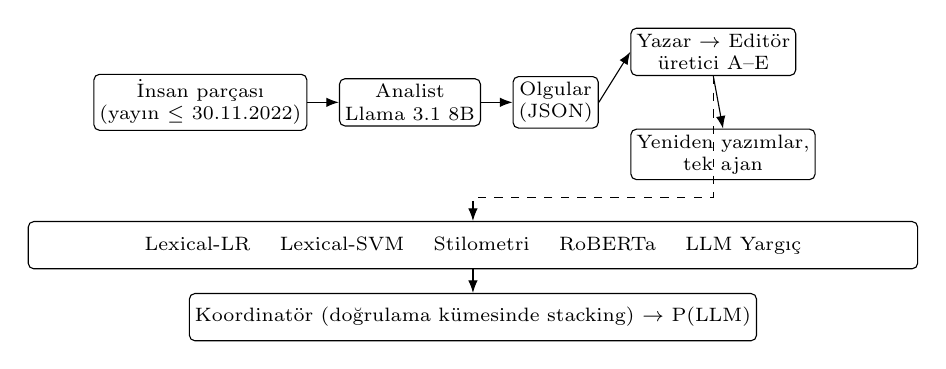
\begin{tikzpicture}[
  box/.style={draw, rounded corners=2pt, align=center, font=\scriptsize, minimum height=6mm, inner sep=2pt},
  arr/.style={-{Latex[length=1.6mm]}, thin}]
\node[box] (h) {İnsan parçası\\(yayın $\le$ 30.11.2022)};
\node[box, right=4mm of h] (an) {Analist\\Llama 3.1 8B};
\node[box, right=4mm of an] (f) {Olgular\\(JSON)};
\node[box, above right=0mm and 4mm of f] (w) {Yazar $\rightarrow$ Editör\\üretici A--E};
\node[box, below right=0mm and 4mm of f] (s) {Yeniden yazımlar,\\tek ajan};
\draw[arr] (h) -- (an);
\draw[arr] (an) -- (f);
\draw[arr] (f.east) -- (w.west);
\draw[arr] (w.south) -- (s.north);
\node[box, below=12mm of an, xshift=8mm, text width=0.92\columnwidth]
  (d) {Lexical-LR \quad Lexical-SVM \quad Stilometri \quad RoBERTa \quad LLM Yargıç};
\node[box, below=3mm of d] (c) {Koordinatör (doğrulama kümesinde stacking) $\rightarrow$ P(LLM)};
\draw[arr] (d) -- (c);
\draw[arr, dashed] (w.south) |- ([yshift=3mm]d.north) -- (d.north);
\end{tikzpicture}
\caption{Üretim ajanları (üstte) ve tespit ajanları (altta). Bütün üreticiler aynı Analist olgularından yazar ve insan
parçasını hiç görmez. Yeniden yazılmış sürümler Yazar--Editör çıktısından başlar; tek ajan koşulu insan parçasını
doğrudan okur. İnsan parçaları CISA'dan (eğitim ve test) ve Microsoft ile Mandiant'tan (yalnızca test) gelir.}
\label{fig:pipeline}
\end{figure}

Şekil~\ref{fig:pipeline} hattı özetliyor. Her ajan, bir modele bağlanmış bir rol promptundan ibaret. Bir mesaj alıyor
ve bir mesaj döndürüyor. \emph{Analist} bir insan parçasını okuyor ve içerdiği olguları on anahtarlı bir JSON olarak
döndürüyor (aktör, zararlı yazılım, CVE'ler, TTP'ler, hedefler, sektörler, gösterge türleri, zaman çizelgesi, etki,
önlemler). Parçanın söz etmediği anahtarı boş bırakması isteniyor. Her parça için bir kez, yerel Llama~3.1~8B
üzerinde JSON kısıtlı çıktı ve 0.2 sıcaklıkla çalışıyor. Her üretici için bir \emph{Yazar}, olguları ve insan
parçasının uzunluğuna eşit bir hedef uzunluğu alıp bir CTI metni yazıyor. Ardından bir \emph{Editör} olguları ve
taslağı alıyor ve taslağı, yeni olgu eklememe talimatıyla, olgulara göre düzeltiyor. Yazar promptu dört şablondan
biri (SOC bülteni, güvenlik firması blogu, devlet bildirimi, olay müdahale raporu), örnekleme sıcaklığı 0.7 veya
1.0. İkisi de üretici ve parçayla tohumlanan bir rastgele sayı üretecinden çekiliyor. Böylece yarıda kalan bir
çalıştırma aynı seçimlerle sürüyor. Seçimler, bütün ajan mesajları ve model adıyla birlikte her metinle
saklanıyor. Boş gelen ya da ret cümlesiyle başlayan bir cevap en çok üç kez yeniden isteniyor. Sonra parça o
üretici için atlanıyor.

Eğitim üreticileri Ollama ile yerelde çalışıyor: A, Llama~3.1~8B (Meta); B, Qwen~2.5~7B (Alibaba); C, Mistral~7B
(Mistral AI). Daha büyük iki API modeli yalnızca görülmemiş test üreticisi olarak kullanılıyor: D, gpt-oss-120b
(OpenAI ağırlıkları, Groq API) ve E, Gemini~3.1~Flash-Lite (Google API). Ücretsiz katmanları günde yaklaşık 200 bin
token ve 500 istek veriyor. Bu yüzden kısıtsız bir ilk çalıştırmadan sonra D ve E'yi, kaynağı en az bir seed'in
test kümesine düşen parçalarla ve çok ajanlı koşulla sınırladık. Bu \NVarChunks{} parçanın hepsinin D ve E sürümü
var. Kısıtlamadan önce üretilmiş metinlerle birlikte kapsam, bütün parçaların \NCoverD{} ve \NCoverE{} kadarına
çıkıyor. Bu fazladan metinler eğitimde hiç kullanılmıyor, yalnızca derlem istatistiklerine giriyor. Kaynakların
sabit bir \SingleShare{} kadarı için her yerel üretici bir de \emph{tek ajan} sürümü yazıyor: insan parçasını okuyup
tek çağrıda yeniden yazan bir ajan. Dış yayıncıların parçaları da aynı hatla A, B ve C'den LLM sürümleri alıyor.

\subsection{Yeniden yazım, prompt stratejileri ve kısmi üretim}
Kaynağı en az bir seed'in test kümesinde bulunan her parça için A, B ve C'nin çok ajanlı metinlerinden yeni LLM
metinleri türettik (Tablo~\ref{tab:robustness} bunları listeliyor). Beş koşul bitmiş bir metni yeniden yazıyor:
\emph{aynı modelle yeniden ifade} (üretici kendi metnini her olguyu, adı ve sayıyı koruma talimatıyla yeniden
yazıyor), \emph{başka modelle yeniden ifade} (A'nın metnini B, B'ninkini C, C'ninkini A yeniden yazıyor), \emph{iki
kez yeniden ifade} (aynı modelle yapılan yeniden ifadenin bir kez daha yeniden ifade edilmesi), Almanca üzerinden
\emph{geri çeviri} ve ulusal bir CERT'te çalışan deneyimli bir analistin dilini, birinci şahıs ve okura tavsiye
olmadan isteyen bir \emph{``insanlaştır''} promptu. İki prompt stratejisi Yazar'ı değiştiriyor: bir devlet
bildiriminin kişisiz dilini isteyen \emph{bildiri üslubu} promptu ve hiçbir seed'in test kümesinde bulunmayan
kaynaklardan alınmış iki insan parçası gösteren \emph{az örnekli} prompt. \emph{Yalnızca Yazar} koşulu, taslağın
Editör'den önceki hâli. Üçüncü ajanın neyi değiştirdiğini ölçüyor. Son olarak \emph{kısmen üretilmiş} metinler, bir
insan parçasının cümleleriyle onun LLM sürümünün cümlelerini, LLM cümleleri kelimelerin yaklaşık \%25'ini,
\%50'sini veya \%75'ini oluşturacak biçimde birleştiriyor. RoBERTa yalnızca ilk 256 tokenı okuduğu için LLM bloğu
rastgele başa veya sona yerleştiriliyor. Toplamda bu adım \NVarTexts{} LLM metni ekliyor. Kısmen üretilmiş her metni
LLM olarak etiketliyoruz. Bu bir kabul: kelimelerinin dörtte biri LLM'den gelen bir metin çoğunlukla insan metni ve
bu metinlerdeki ``duyarlılık'', bir dedektörün tepki vermesi için araya ne kadar LLM metni girmesi gerektiğini
ölçüyor.

İnsanların LLM taslaklarını düzelttiği, insan tarafından düzenlenmiş bir küme oluşturmadık. Bu tür düzenlemeleri
başka bir LLM ile taklit etmek LLM yeniden yazımını ikinci kez ölçmek olurdu. Bu koşulu sonraki çalışmaya bırakıyor
ve en yakın vekil olarak cümle düzeyindeki karışımları kullanıyoruz (Bölüm~\ref{sec:limits}).

\subsection{Ön işleme ve bölme}
LLM çıktıları metnin parçası olmayan ambalajlar içeriyor: akıl yürütme etiketleri, ``Here is the revised text'' gibi
girişler, başlıklar, markdown, madde işaretleri ve kelime sayısı notları. Bunları siliyor ve insan ya da üretilmiş,
bütün metinlerde tire ve tırnakların Unicode varyantlarını normalleştiriyoruz. Bu adımın etkisi bir ablasyonda
ölçülüyor. 50 kelimeden kısa metinler atılıyor.

Bölme kaynak rapor düzeyinde yapılıyor: CISA kaynaklarının \%70'i eğitim, \%10'u doğrulama ve \%20'si test için, her
seed (42, 123, 2024) için ayrı. Bir insan parçası ve yeniden yazılmış olsun olmasın bütün LLM sürümleri her zaman
aynı kümeye düşüyor. Vektörleştiriciler, ölçekleyiciler, dedektörler, Koordinatör, kalibratörler ve eşikler
yalnızca eğitim veya doğrulama verisiyle kuruluyor. Test, D, E, yeniden yazılmış ve dış yayıncı metinleri yalnızca
puanlanıyor.

\section{Tespit Ajanları}\label{sec:agents}
\subsection{Üyeler}
\begin{itemize}
\item \textbf{Lexical-LR} (baseline 1): kelime 1--2-gram ve karakter 3--5-gram TF-IDF ile lojistik regresyon.
\item \textbf{Lexical-SVM} (baseline 2): aynı özelliklerle doğrusal SVM, Platt kalibrasyonlu.
\item \textbf{Stilometri}: beş grupta 32 özellik (uzunluk, MTLD dahil sözcük çeşitliliği \cite{McCarthy_2010},
noktalama, tekrar, sözcük türü oranları) ile XGBoost.
\item \textbf{Transformer}: üç epoch ince ayar yapılmış RoBERTa-base \cite{Liu_2019}, en fazla 256 token.
\item \textbf{LLM Yargıç}: üretimde kullanılmayan bir aileden Gemma~2~9B; bir metnin yapay zekâ tarafından üretilmiş
olma olasılığı sıfır örnekli olarak soruluyor.
\end{itemize}

\subsection{Eğitim gerektirmeyen referans dedektörler}
\emph{Fast-DetectGPT}, koşullu olasılık eğriliğinin analitik biçimini, örnekleme ve puanlama modeli olarak
GPT-Neo~2.7B ile kullanıyor \cite{Bao_2024}. \emph{Binoculars}, yazarların model çiftini kullanıyor: gözlemci olarak
Falcon-7B, icracı olarak Falcon-7B-Instruct \cite{Hans_2024}. İki 7B model 8~GB'lık bir GPU'ya birlikte sığmadığı
için ikisi de 4 bit hassasiyetle yükleniyor ve iki geçişte çalıştırılıyor. Gözlemcinin sonraki token dağılımı en
olası 64 tokena kırpılıp yeniden normalleştirilerek diske yazılıyor, icracı geçişi şaşkınlığı ve çapraz şaşkınlığı
bu dağılımdan hesaplıyor. Kırpma olmadan bu iki geçişli hesap tam skoru yeniden üretiyor. Bunu küçük bir modelde
kontrol ettik. Kırpma ise zararsız değil. Her iki yolla puanlanan \NBinoCheck{} rastgele metnin \BinoHigher{}
tanesinde kırpılmış skor tam skordan yüksek çıktı. Mutlak farkın medyanı \BinoMedDiff{}, tam skorların medyanı
\BinoMedScore{}, iki skor arasındaki sıra korelasyonu ise \BinoRho{} oldu. Yani Binoculars skorlarımız kaymış
durumda, ama metinleri tam skorlarla neredeyse aynı sıraya diziyor. İki yöntem de en çok 512 token okuyor. Eğitim
gerektirmiyorlar ama skorları olasılık değil. Denetimli dedektörlerle aynı eşik kuralları altında
karşılaştırılabilmeleri için bu skorları her eğitim kümesinin doğrulama kısmında, sınıf dengeli Platt ölçeklemeyle
olasılığa çeviriyoruz.

\subsection{Koordinatör}
Koordinatör, beş üyenin olasılıklarının logitleri üzerinde bir lojistik regresyon (yığınlanmış genelleme
\cite{Wolpert_1992}):
\begin{equation}
P(\text{LLM} \mid x) = \sigma\Big(b + \sum_{m=1}^{5} w_m \log\frac{p_m(x)}{1 - p_m(x)}\Big).
\end{equation}
Burada $p_m(x)$, $m$ üyesinin verdiği olasılık, $\sigma$ lojistik fonksiyon. $w_m$ ağırlıkları ve $b$ sabiti, eğitim
üreticilerinin doğrulama kümesiyle, yani üyelerin eğitilmediği veriyle kuruluyor. Ağırlıklar her çalıştırmada
kaydediliyor ve sonuçlarla birlikte veriliyor. Bir yığının neden en iyi üyesinin gerisinde kalabildiğini bulmak
için aynı tahminler üzerinde dört çeşit değerlendiriyoruz: üye logitlerinin ağırlıksız ortalaması (öğrenilmiş
ağırlık yok), doğrulama F1 değeri en yüksek tek üye (birleştirme yerine seçme), eğitim kümesinde \emph{bulunmayan}
yerel üreticilerin doğrulama metinleriyle kurulan bir yığın (ağırlıklar benzetilmiş bir üretici kayması altında
öğreniliyor) ve iki sıfır örnekli dedektörün üye olarak eklendiği yığın.

\subsection{Neden birden çok ajan}\label{sec:why}
\emph{Üretim.} Olgu çıkarmayı yazımdan ayırmak deneyin işine yarıyor. Tek ajan koşulumuzdaki gibi tek bir prompt
insan parçasını okuyup yeniden yazdığında çıktı kaynağın adlarını ve ifadelerini koruyor, üstelik farklı üreticiler
bunların farklı miktarını koruyor. Tek ajanlı bir metnin kelime üçlülerinin, üreticiye göre \OverlapSingleMin{} ile
\OverlapSingleMax{} arasındaki bir kısmı kendi insan parçasında da geçiyor. Aynı parçaların çok ajanlı metinlerinde
bu oran \OverlapMultiMin{} ile \OverlapMultiMax{} arasında. Kalan örtüşme, olgular üzerinden geçen varlık adlarından
ve kalıp ifadelerden geliyor. Tek ajan koşulunda üreticiler arası farklar bu yüzden üslup ile kopyalamayı
karıştırırdı. Ortak bir Analist ile içerik beş üreticide de sabit kalıyor ve insan ifadesi Yazar'a hiç
gösterilmiyor. Editör, insan CTI üretimindeki gibi bir gözden geçirme adımı ekliyor. Etkisi yalnızca Yazar koşuluyla
ölçülüyor. Bedeli metin başına bir yerine üç çağrı.

\emph{Tespit.} Üyeler farklı kanıtlar kullanıyor: yüzeydeki n-gram'lar, üslubun dağılımsal istatistikleri,
bağlamsal temsiller, talimatla eğitilmiş bir modelin yargısı ve referans dedektörler için başka bir dil modeli
altındaki olabilirlik. Bir üretici kayması bunları eşit etkilemiyor. Daha büyük bir üretici insan uzunluğunu
tutturup bir stilometrik ipucunu ortadan kaldırırken, sözcüksel modellerin kullandığı düşük özel ad oranını
koruyabilir. Üye hataları tam ilişkili değilse öğrenilmiş bir birleşim her üyeden daha doğru olabilir. Aynı
gerekçe birleşimin nerede başarısız olacağını da söylüyor. Eğitim üreticilerinin doğrulama metinleriyle kurulan
ağırlıklar orada en güvenilir olan üyeyi ödüllendiriyor. Bu üye, yeni koşula en iyi taşınan üye olmak zorunda
değil. Yukarıdaki çeşitler bunu doğrudan sınıyor; Bölüm~\ref{sec:results} birleşimin ne zaman yardımcı olduğunu ve
ne zaman olmadığını veriyor.

\section{Deney Düzeni}\label{sec:setup}
\subsection{Senaryolar}
Yerel üreticilerin boş olmayan her alt kümesi (A, B, C, AB, AC, BC, ABC) ve her seed için bir eğitim yapılıyor ve
eğitilen her model her üreticinin test kümesinde deneniyor. Aynı eğitimlerden dört düzen çıkıyor: \emph{E1 aynı
üretici} (aynı üreticiyle eğitim ve test, ayrıca birleşik ABC modeli), \emph{E2 üreticiler arası} (birinde eğitim,
diğerinde test; ödevde istenen İnsan+A $\rightarrow$ İnsan+B ve İnsan+A $\rightarrow$ İnsan+C durumları bunun
içinde), \emph{E3 birini dışarıda bırak} (ikisinde eğitim, üçüncüsünde test) ve \emph{E4 dış üretici} (herhangi bir
eğitim kümesi, D veya E ile test). Her test kümesi bir üreticinin test kaynaklarına ait LLM metinlerini ve bunların
üretildiği insan parçalarını içeriyor. Sınıflar bu yüzden dengeli.

Aynı eğitimler dış yayıncıları ve yeniden yazılmış metinleri de puanlıyor. \emph{Yayıncı kayması}, Microsoft ve
Mandiant'ın bütün insan parçalarındaki yanlış pozitif oranıyla ve bu parçaların A, B ve C sürümleriyle
eşleştirildiği kümede duyarlılık, F1 ve ROC-AUC ile ölçülüyor. \emph{Yeniden yazım ve kısmi üretim}, türetilmiş
metinlerdeki duyarlılıkla ölçülüyor ve aynı parçaların çok ajanlı metinlerindeki duyarlılıkla karşılaştırılıyor.
Tek ajan koşulu aynı modelin aynı parçalara ait çok ajanlı metinleriyle karşılaştırılıyor. Her biri üç seed ile
yapılan iki genişletilmiş eğitim, daha çeşitli eğitim verisinin yardımcı olup olmadığını sınıyor: ABC artı bir dış
yayıncı (insan ve LLM sürümleri) ile eğitip diğer yayıncıda test, ve ABC artı eğitim kaynaklarının yeniden ifade
edilmiş ve tek ajanlı metinleri.

\subsection{Metrikler ve istatistik}
Doğruluk, kesinlik, duyarlılık, F1, makro-F1, ROC-AUC ve PR-AUC değerlerini üç seed üzerinden ortalama $\pm$
standart sapma olarak veriyoruz. Aralıklar ve testler kaynak rapor düzeyinde çalışıyor. Test kaynakları yerine
koyarak yeniden örnekleniyor (2{.}000 bootstrap örneği). Bu, bir metrik için \%95 yüzdelik aralığı veriyor. Bir
karşılaştırmada metrik farkı iki sistem için aynı yeniden örneklenmiş kaynaklar üzerinde hesaplanıyor. Bu da
eşleştirilmiş bir aralık ve çift yönlü bir $p$ değeri veriyor. 2{.}000 örnekle böyle bir $p$ değeri en az $2/2001$
olabiliyor. Dolayısıyla Holm düzeltmesi \cite{Holm_1979} elliden fazla testlik bir ailede hiçbir şeyi reddedemiyor.
Bu yüzden bir karşılaştırmanın çalıştırmalarını testten önce havuzluyoruz: aynı üretici ile başka üretici
arasındaki fark için dedektör ve hedef başına bir test, Koordinatör ile RoBERTa için senaryo başına bir test,
yeniden yazım koşulları için koşul ve dedektör başına bir test. Holm yöntemi bu ailelerin her birinin içinde
uygulanıyor. Testlerin çalıştırma veya özellik başına verildiği yerlerde Benjamini-Hochberg yöntemi
\cite{Benjamini_1995} kullanılıyor. Dedektörler tek tek test kümelerinde kesin McNemar testiyle de
karşılaştırılıyor. Düzeltme dedektör çifti başına Holm ile. Dilsel farklar Mann-Whitney U testi ve etki büyüklüğü
olarak Cliff $\delta$ ile sınanıyor. Ayırt edici n-gram'lar ağırlıklı log-odds ile sıralanıyor \cite{Monroe_2008}.

\subsection{Kalibrasyon ve eşikler}
Her dedektör ve eğitim için doğrulama kümesinde üç kalibratör kuruyoruz: Platt ölçekleme (skorun logiti üzerinde
lojistik regresyon) \cite{Platt_1999}, sıcaklık ölçekleme (doğrulama log-kaybıyla seçilen tek bir logit böleni)
\cite{Guo_2017} ve izotonik regresyon \cite{Zadrozny_2002}. Koordinatör de doğrulama kümesinde kurulduğu için
kalibratörleri, kaynağa göre gruplanmış beş katlı bir bölmeden gelen kat dışı yığın skorlarını kullanıyor. Olasılık
kalitesi test kümelerinde Brier skoru, 15 eşit genişlikte kutulu beklenen kalibrasyon hatası \cite{Naeini_2015} ve
negatif log-olabilirlik ile ölçülüyor ve güvenilirlik diyagramlarıyla gösteriliyor (Şekil~\ref{fig:reliability}).

Hepsi doğrulama verisinde belirlenen beş karar kuralı karşılaştırılıyor: sabit 0.5 eşiği; doğrulama F1 değerini en
yükseğe çıkaran eşik; ne eğitim kümesinde ne de test üreticisi olan yerel üreticilerin doğrulama metinlerinde F1'i
en yükseğe çıkaran \emph{sözde görülmemiş} eşik; ve iki \emph{insan yüzdeliği} eşiği. Bunlar doğrulama insan
skorlarının 99. ve 95. yüzdelikleri; \%1 veya \%5 yanlış pozitif oranını hedefliyor ve hiç LLM metni kullanmıyorlar.
Son iki kural test sırasında karşılaşılacak üretici hakkında hiçbir şey varsaymıyor. Varsaydıkları şey, test
sırasındaki insan metninin CISA doğrulama metni gibi skor alacağı; dış yayıncılar bu varsayımı sınıyor.

\subsection{Maliyet}
Çıkarım süresi tek bir dizüstü RTX~4060 (8~GB) üzerinde, sabit bir test metni örneğinde, üç tekrarla ve GPU'da
başka bir şey çalışmazken ölçülüyor. LLM yargıç daha küçük bir örnekte ölçülüyor. Eğitim süresi her çalıştırmada
kaydediliyor. Koordinatör'ün maliyeti, üyelerinin art arda çalıştırılmasının toplamı.

\subsection{Hata analizi}\label{sec:errors}
Yanlış negatifler (insan olarak puanlanan LLM metinleri), tek bir yerel üreticiyle eğitilen modellerden, bütün
seed'ler üzerinden alınıyor. Çünkü D bu modellerde kaçıyor. Yanlış pozitifler (LLM olarak puanlanan insan metinleri)
CISA için aynı modellerden, firma parçaları için ise birleşik ABC modellerinden alınıyor. Çünkü yanlış alarmlar
orada ortaya çıkıyor. Her metin için uzunluğu, MTLD'yi, tür-örnek oranını, özel ad ve zamir oranlarını, birinci
şahıs zamirlerini (\emph{we, our, us, ours}), kurum adlarını, tavsiye bildiren sözcükleri, Analist olgularında
bulunmayan teknik tanımlayıcıları (dosya adları, CVE numaraları, adresler, ATT\&CK kimlikleri) ve \emph{ipucu}
oranını hesaplıyoruz. İpucu oranı, A ile eğitilen Lexical-LR'de en büyük pozitif ağırlığı alan 30 ve en büyük
negatif ağırlığı alan 30 terim arasındaki kelime n-gram'larının (sırasıyla \NCueLlm{} ve \NCueHuman{} tane) 100
kelimedeki geçiş sayısı.

Bu özelliklerle üç analiz yapıyoruz. Birincisinde her hata, uyan ilk kurala göre tek bir kategoriye atanıyor ve her
kategorinin hatalar içindeki payı, aynı gruptaki bütün metinler içindeki payının yanında veriliyor. İkinci sayı
olmadan, yalnızca üreticiyi betimleyen bir kategori bir neden gibi görünürdü. İkincisinde yanlış sınıflandırılan
metinler doğru sınıflandırılanlarla özellik özellik karşılaştırılıyor (Mann-Whitney U, Cliff $\delta$,
Benjamini-Hochberg). Her çalıştırmada kaçan bir metin dokuz kez sayılmasın diye önce her metnin çalıştırmalar
üzerinden ortalaması alınıyor. Üçüncüsünde hata göstergesinin standartlaştırılmış özellikler üzerindeki, standart
hataları kaynağa göre kümelenmiş lojistik regresyonu, diğerleri sabitken hangi özelliklerin hata olasılık oranını
değiştirdiğini kestiriyor. Kuralları tek bir yazar tanımladı. İkinci bir işaretleyiciyle doğrulanmadılar.

\section{Sonuçlar}\label{sec:results}
\begin{table*}[t]
\centering
\footnotesize
\caption{Kaynağa göre derlem. Medyanlar çok ajanlı metinler üzerinden (ilk satırda insan parçaları).}
\label{tab:data}
\begin{tabular}{lrrrrrr}
\toprule
Kaynak & Çok ajan & Tek ajan & Kelime & MTLD & Tekrar bigram & PROPN \\
\midrule
İnsan (CISA) & 406 & 0 & 302 & 84 & 0.094 & 0.114 \\
A: Llama 3.1 8B & 406 & 83 & 163 & 90 & 0.065 & 0.050 \\
B: Qwen 2.5 7B & 405 & 83 & 147 & 121 & 0.033 & 0.055 \\
C: Mistral 7B & 406 & 83 & 214 & 132 & 0.039 & 0.059 \\
D: gpt-oss-120b & 248 & 0 & 306 & 199 & 0.029 & 0.049 \\
E: Gemini 3.1 Flash-Lite & 305 & 0 & 300 & 169 & 0.031 & 0.033 \\
\bottomrule
\end{tabular}
\end{table*}

\subsection{Dilsel farklar}
Tablo~\ref{tab:data} ve Şekil~\ref{fig:boxes} derlemi özetliyor. \NTests{} üretici-özellik karşılaştırmasının
\NLargeEffects{} tanesinde, Benjamini-Hochberg düzeltmesinden sonra da büyük bir etki ($|\delta| \geq 0.474$)
kalıyor. En tutarlı fark sözcük çeşitliliğinde. Medyan MTLD, CISA parçalarında \MedMtldHuman{}. Üreticilerde
\MedMtldA{} ile \MedMtldD{} arasında. Hapax oranı her üreticide insandan yüksek ($\delta$ \HapaxDeltaMin{} ile
\HapaxDeltaMax{} arası). LLM metinleri daha az bigram tekrarlıyor ve daha az özel ad kullanıyor. İnsan parçaları
kurumları, ürünleri, dosyaları ve tarihleri tekrar tekrar adıyla anıyor. Üreticiler aynı olguları genel ifadelerle
aktarıyor. Yerel üreticiler ayrıca kısa yazıyor (medyan \MedWordsA{}, \MedWordsB{} ve \MedWordsC{} kelime; insanda
\MedWordsHuman{}), D ve E ise insan uzunluğunu tutturuyor (\MedWordsD{} ve \MedWordsE{}). Log-odds sıralaması da
aynı yönü gösteriyor. LLM metinleri \emph{our}, \emph{we}, \emph{potential}, \emph{to mitigate} ve \emph{defenders
should} gibi okura tavsiye veren ifadeleri sık kullanıyor. CISA parçalarında ise atıf ve çapraz gönderme bildiren
\emph{CISA}, \emph{FBI}, \emph{see} ve \emph{note} sık geçiyor. Tek tek özellikler düzeyinde H1 beş üreticinin
hepsinde geçerli.

İki firma yayıncısı bu özelliklerin bir kısmında CISA ile üreticilerin arasında kalıyor. Microsoft ve Mandiant
parçaları CISA'ya göre daha çok zamir ($\delta = \PubMicrosoftPosPronDelta$ ve $\PubMandiantPosPronDelta$), daha az
özel ad ($\delta = \PubMicrosoftPosPropnDelta$ ve $\PubMandiantPosPropnDelta$) kullanıyor; LLM metni de CISA'dan bu
yönde ayrılıyor. \NPubTests{} yayıncı-özellik karşılaştırmasının \NPubLarge{} tanesinde etki büyük.

\begin{figure*}[t]
\centering
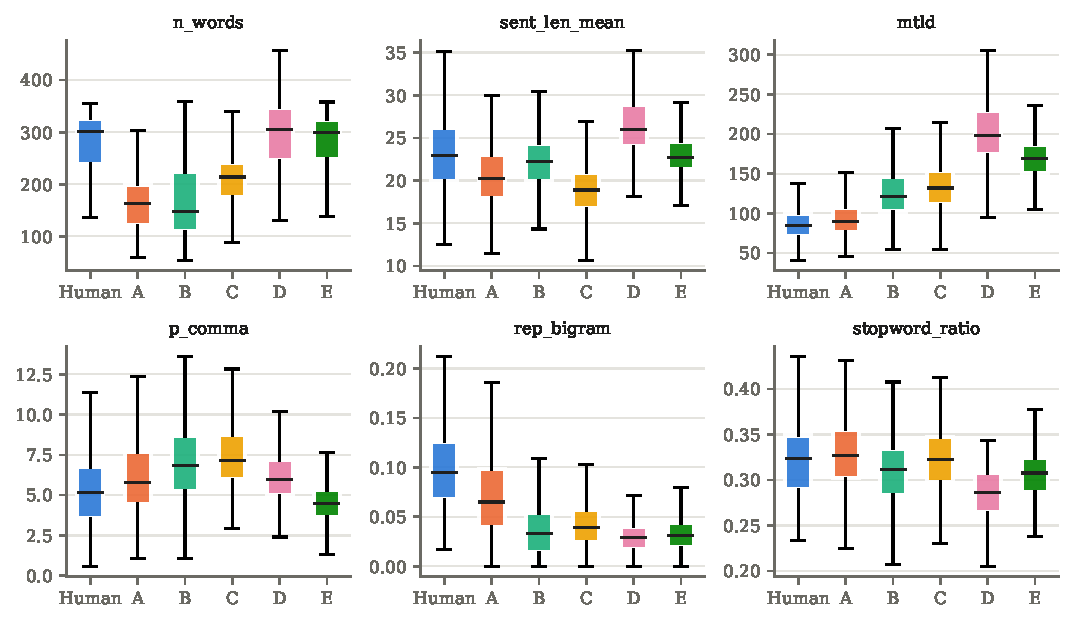
\includegraphics[width=\textwidth]{feature_boxes.pdf}
\caption{CISA parçaları ve beş üretici (çok ajanlı metinler) için seçilmiş stilometrik özellikler.}
\label{fig:boxes}
\end{figure*}

\begin{table*}[t]
\centering
\footnotesize
\caption{Tek bir üreticiyle (A, B veya C) eğitilen modeller. F1, eğitim üreticileri ortalamasının üç seed üzerinden ortalama $\pm$ standart sapmasıdır; AUC, ROC-AUC'dir.}
\label{tab:main}
\begin{tabular}{lcccccccc}
\toprule
Dedektör & \multicolumn{2}{c}{Aynı üretici} & \multicolumn{2}{c}{Çapraz (A--C)} & \multicolumn{2}{c}{D: gpt-oss-120b} & \multicolumn{2}{c}{E: Gemini} \\
 & F1 & AUC & F1 & AUC & F1 & AUC & F1 & AUC \\
\midrule
Lexical-LR & 0.997 $\pm$ 0.004 & 1.000 & 0.966 $\pm$ 0.009 & 1.000 & 0.336 $\pm$ 0.032 & 0.976 & 0.960 $\pm$ 0.013 & 1.000 \\
Lexical-SVM & 0.998 $\pm$ 0.004 & 1.000 & 0.975 $\pm$ 0.004 & 1.000 & 0.351 $\pm$ 0.036 & 0.982 & 0.969 $\pm$ 0.012 & 1.000 \\
Stilometri & 0.935 $\pm$ 0.009 & 0.983 & 0.869 $\pm$ 0.010 & 0.956 & 0.704 $\pm$ 0.010 & 0.875 & 0.784 $\pm$ 0.015 & 0.926 \\
RoBERTa & 0.991 $\pm$ 0.002 & 0.999 & 0.989 $\pm$ 0.002 & 0.999 & 0.845 $\pm$ 0.061 & 0.984 & 0.988 $\pm$ 0.005 & 0.999 \\
LLM Yargıç & 0.504 $\pm$ 0.024 & 0.409 & 0.504 $\pm$ 0.024 & 0.409 & 0.499 $\pm$ 0.026 & 0.533 & 0.628 $\pm$ 0.015 & 0.754 \\
Fast-DetectGPT & 0.748 $\pm$ 0.004 & 0.828 & 0.729 $\pm$ 0.015 & 0.828 & 0.566 $\pm$ 0.027 & 0.699 & 0.457 $\pm$ 0.019 & 0.613 \\
Binoculars & 0.815 $\pm$ 0.023 & 0.900 & 0.804 $\pm$ 0.016 & 0.900 & 0.390 $\pm$ 0.048 & 0.734 & 0.330 $\pm$ 0.087 & 0.671 \\
Koordinatör & 0.996 $\pm$ 0.001 & 1.000 & 0.993 $\pm$ 0.005 & 1.000 & 0.732 $\pm$ 0.089 & 0.988 & 0.993 $\pm$ 0.010 & 1.000 \\
\bottomrule
\end{tabular}
\end{table*}

\subsection{Aynı üretici ve üreticiler arası tespit}
Tek bir üreticiyle eğitilen modellerin ana sonucu Tablo~\ref{tab:main}'de. Aynı üreticide tespit neredeyse
kusursuz: F1, sözcüksel baseline'larda \FoneInLexLR{}, RoBERTa'da \FoneInTrans{}, Koordinatör'de \FoneInCoord{}.
Başka bir yerel üreticiye geçmek az kaybettiriyor (Lexical-LR \FoneCrossLexLR{}, RoBERTa \FoneCrossTrans{}). İki
üreticiyle eğitilip üçüncüsünde sınanan modellerde de sonuç benzer (Lexical-LR \LooLexLR{}, RoBERTa \LooTrans{}).
Bu dedektörler Gemini (E) metinlerini de neredeyse aynı başarıyla buluyor. Büyük düşüş gpt-oss-120b'de (D).
Lexical-LR'nin F1 değeri \FoneDLexLR{} (\%95 GA [\FoneDLoLexLR{}, \FoneDHiLexLR{}]), Lexical-SVM'inki
\FoneDLexSVM{}; RoBERTa \FoneDTrans{} ([\FoneDLoTrans{}, \FoneDHiTrans{}]), Koordinatör \FoneDCoord{}
([\FoneDLoCoord{}, \FoneDHiCoord{}]) ile tutunuyor. Bütün eğitim kümeleri Şekil~\ref{fig:heatmap}'te.

Lexical-LR, D metinlerini hâlâ insan metinlerinin üstüne sıralıyor (AUC \AucDLexLR{}), ama sabit eşikte bunların
ancak \ThrDLexlrFixedRecall{} kadarını yakalıyor. Şekil~\ref{fig:ecdf}'de D skorları insan parçalarıyla yerel
üreticiler arasında ayrı bir bant oluşturuyor ve çoğu 0.5'in altında kalıyor. Daha düşük bir eşik bunları insan
metinlerinden ayırabilirdi. Daha çok üreticiyle eğitim sınırı kaydırıyor. İki üreticiyle Lexical-LR'nin D'deki F1
değeri \PoolTwoDLexLR{}, üçüyle \PoolDLexLR{} oluyor. Üç üreticiyle RoBERTa \PoolDTrans{}, Koordinatör
\PoolDCoord{} değerine ulaşıyor.

Eğitim gerektirmeyen iki dedektör, aynı üreticide bile denetimli dedektörlerin çok gerisinde (AUC: Fast-DetectGPT
\AucInFast{}, Binoculars \AucInBino{}). Büyük üreticilerde sıralamaları daha da bozuluyor (D'de \AucDFast{} ve
\AucDBino{}, E'de \AucEFast{} ve \AucEBino{}). LLM Yargıç şans düzeyine yakın (F1 \FoneInJudge{}). Aynı üreticideki
AUC değeri (\AucInJudge{}) 0.5'in altında, çünkü CISA test parçalarının \JudgeHumanFlag{} kadarını yapay zekâ
yazımı sayıyor. Bu oran bazı üreticilerin metinlerindekinden yüksek.

\begin{figure*}[t]
\centering
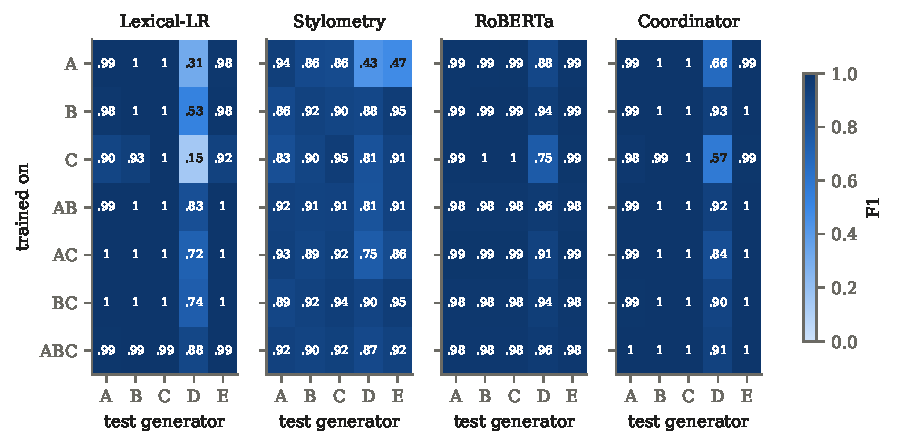
\includegraphics[width=\textwidth]{cross_generator_heatmap.pdf}
\caption{Her eğitim kümesi (satırlar) ve test üreticisi (sütunlar) için F1, üç seed ortalaması. D ve E eğitimde hiç
kullanılmıyor.}
\label{fig:heatmap}
\end{figure*}

\begin{figure}[t]
\centering
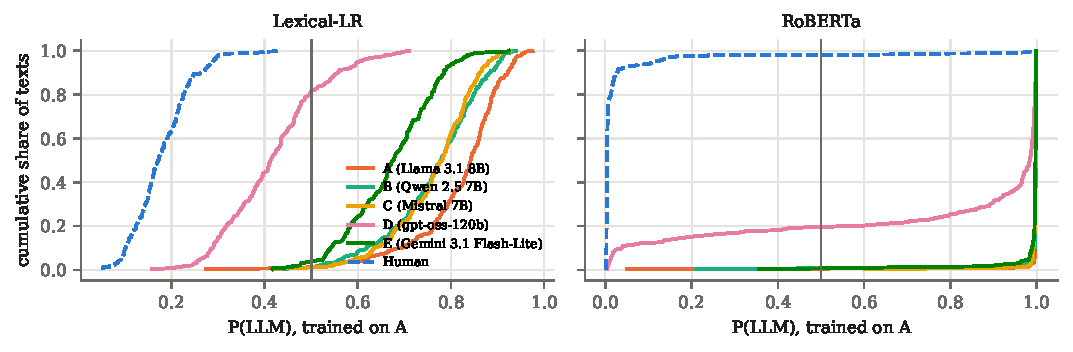
\includegraphics[width=\columnwidth]{score_ecdf.pdf}
\caption{A ile eğitilen modellerde P(LLM) değerinin birikimli dağılımı. İnsan parçaları (kesikli çizgi) ve her
üreticinin metinleri; dikey çizgi sabit eşik.}
\label{fig:ecdf}
\end{figure}

\begin{table*}[t]
\centering
\footnotesize
\caption{İnsan + A ile eğitim, İnsan + her üretici ile test (seed'ler üzerinden ortalama $\pm$ std).}
\label{tab:required}
\begin{tabular}{llccccccc}
\toprule
Test & Dedektör & Doğruluk & Kesinlik & Duyarlılık & F1 & Makro-F1 & ROC-AUC & PR-AUC \\
\midrule
A & Lexical-LR & 0.994 $\pm$ 0.006 & 1.000 $\pm$ 0.000 & 0.988 $\pm$ 0.013 & 0.994 $\pm$ 0.006 & 0.994 $\pm$ 0.006 & 1.000 $\pm$ 0.000 & 1.000 $\pm$ 0.000 \\
A & RoBERTa & 0.987 $\pm$ 0.014 & 0.979 $\pm$ 0.027 & 0.996 $\pm$ 0.007 & 0.987 $\pm$ 0.013 & 0.987 $\pm$ 0.014 & 1.000 $\pm$ 0.000 & 1.000 $\pm$ 0.000 \\
A & Koordinatör & 0.994 $\pm$ 0.000 & 0.992 $\pm$ 0.007 & 0.996 $\pm$ 0.007 & 0.994 $\pm$ 0.000 & 0.994 $\pm$ 0.000 & 1.000 $\pm$ 0.000 & 1.000 $\pm$ 0.000 \\
B & Lexical-LR & 0.996 $\pm$ 0.004 & 1.000 $\pm$ 0.000 & 0.991 $\pm$ 0.008 & 0.996 $\pm$ 0.004 & 0.996 $\pm$ 0.004 & 1.000 $\pm$ 0.000 & 1.000 $\pm$ 0.000 \\
B & RoBERTa & 0.987 $\pm$ 0.012 & 0.979 $\pm$ 0.027 & 0.996 $\pm$ 0.007 & 0.987 $\pm$ 0.012 & 0.987 $\pm$ 0.012 & 1.000 $\pm$ 0.001 & 1.000 $\pm$ 0.001 \\
B & Koordinatör & 0.996 $\pm$ 0.004 & 0.992 $\pm$ 0.007 & 1.000 $\pm$ 0.000 & 0.996 $\pm$ 0.004 & 0.996 $\pm$ 0.004 & 1.000 $\pm$ 0.000 & 1.000 $\pm$ 0.000 \\
C & Lexical-LR & 0.996 $\pm$ 0.004 & 1.000 $\pm$ 0.000 & 0.991 $\pm$ 0.008 & 0.996 $\pm$ 0.004 & 0.996 $\pm$ 0.004 & 1.000 $\pm$ 0.000 & 1.000 $\pm$ 0.000 \\
C & RoBERTa & 0.989 $\pm$ 0.014 & 0.979 $\pm$ 0.027 & 1.000 $\pm$ 0.000 & 0.989 $\pm$ 0.014 & 0.989 $\pm$ 0.014 & 1.000 $\pm$ 0.001 & 1.000 $\pm$ 0.001 \\
C & Koordinatör & 0.996 $\pm$ 0.004 & 0.992 $\pm$ 0.007 & 1.000 $\pm$ 0.000 & 0.996 $\pm$ 0.004 & 0.996 $\pm$ 0.004 & 1.000 $\pm$ 0.000 & 1.000 $\pm$ 0.000 \\
D & Lexical-LR & 0.593 $\pm$ 0.004 & 1.000 $\pm$ 0.000 & 0.185 $\pm$ 0.009 & 0.313 $\pm$ 0.012 & 0.512 $\pm$ 0.007 & 0.980 $\pm$ 0.018 & 0.980 $\pm$ 0.019 \\
D & RoBERTa & 0.894 $\pm$ 0.065 & 0.977 $\pm$ 0.029 & 0.810 $\pm$ 0.149 & 0.879 $\pm$ 0.087 & 0.892 $\pm$ 0.069 & 0.977 $\pm$ 0.017 & 0.977 $\pm$ 0.018 \\
D & Koordinatör & 0.747 $\pm$ 0.047 & 0.983 $\pm$ 0.016 & 0.503 $\pm$ 0.093 & 0.662 $\pm$ 0.084 & 0.730 $\pm$ 0.057 & 0.972 $\pm$ 0.014 & 0.972 $\pm$ 0.016 \\
E & Lexical-LR & 0.981 $\pm$ 0.001 & 1.000 $\pm$ 0.000 & 0.962 $\pm$ 0.002 & 0.981 $\pm$ 0.001 & 0.981 $\pm$ 0.001 & 1.000 $\pm$ 0.000 & 1.000 $\pm$ 0.000 \\
E & RoBERTa & 0.987 $\pm$ 0.012 & 0.979 $\pm$ 0.027 & 0.996 $\pm$ 0.007 & 0.987 $\pm$ 0.012 & 0.987 $\pm$ 0.012 & 1.000 $\pm$ 0.001 & 1.000 $\pm$ 0.001 \\
E & Koordinatör & 0.994 $\pm$ 0.000 & 0.992 $\pm$ 0.007 & 0.996 $\pm$ 0.007 & 0.994 $\pm$ 0.000 & 0.994 $\pm$ 0.000 & 1.000 $\pm$ 0.000 & 1.000 $\pm$ 0.000 \\
\bottomrule
\end{tabular}
\end{table*}

Çalıştırmalar havuzlandığında, eğitim üreticisinden başka bir yerel üreticiye geçişte kaybedilen F1, Lexical-LR'de
\HpCrossLexLR{} (\%95 GA [\HpLoCrossLexLR{}, \HpHiCrossLexLR{}]), RoBERTa'da \HpCrossTrans{} ([\HpLoCrossTrans{},
\HpHiCrossTrans{}]). Holm düzeltmesinden sonra kayıp, eğitilmiş ve eğitimsiz \HpNCross{} dedektörün \HpSigCross{}
tanesinde anlamlı. İstisnalar RoBERTa ve Binoculars. D'de kayıp Lexical-LR'de \HpDLexLR{}, RoBERTa'da \HpDTrans{},
Koordinatör'de \HpDCoord{} ve \HpND{} dedektörün hepsinde anlamlı. E'de \HpNE{} dedektörün \HpSigE{} tanesinde
anlamlı; RoBERTa ve Koordinatör ölçülebilir bir kayıp vermiyor. Çalıştırma çalıştırma sınandığında,
Benjamini-Hochberg düzeltmesinden sonra \HoneNCross{} yerel karşılaştırmanın \HoneSigCross{} tanesi, D ve E'deki
\HoneNExt{} karşılaştırmanın \HoneSigExt{} tanesi anlamlı kalıyor. Tek tek test kümelerindeki kesin McNemar testleri
de bu tabloyla uyumlu. Holm düzeltmesinden sonra RoBERTa \McTransLexN{} test kümesinin \McTransLexSig{} tanesinde
Lexical-LR'den, Koordinatör \McCoordLexSig{} tanesinde Lexical-LR'den, \McCoordTransSig{} tanesinde RoBERTa'dan
farklı.

Ödevde istenen düzenin, İnsan + A ile eğitimin bütün metrikleri Tablo~\ref{tab:required}'de; Koordinatör'ün seed 42
için karmaşıklık matrisleri Şekil~\ref{fig:cm}'de. Koordinatör A'da \CmAFP{} yanlış pozitif ve \CmAFN{} yanlış
negatif yapıyor (TP \CmATP{}, TN \CmATN{}). D'de yanlış pozitif sayısı yine \CmDFP{}, ama
\the\numexpr\CmDTP+\CmDFN\relax{} LLM metninin \CmDFN{} tanesi kaçıyor. Bir CTI hattında pahalı olan hata yanlış
negatif. Kaçırılan sahte rapor bilgi tabanına giriyor ve istihbarat diye paylaşılıyor. Yanlış pozitifin bedeli ise
bir analistin metne ikinci kez bakması.

\begin{figure*}[t]
\centering
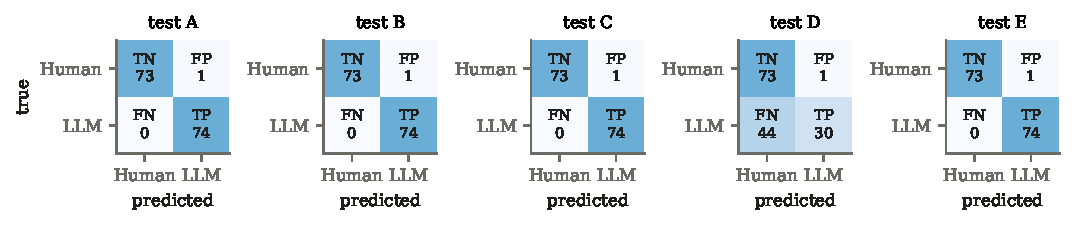
\includegraphics[width=\textwidth]{confusion_coordinator.pdf}
\caption{İnsan + A ile eğitilen Koordinatör (seed 42), her üreticide test.}
\label{fig:cm}
\end{figure*}

\begin{table*}[t]
\centering
\footnotesize
\caption{CISA + ABC ile eğitilen modeller, eşik 0.5. FPR yayıncının bütün insan parçaları üzerinde; duyarlılık, F1 ve AUC insan parçaları ile bunların A, B ve C sürümleri üzerinde, ortalama. FPR ve F1 üç seed üzerinden ortalama $\pm$ std; aralık kaynakları yeniden örnekler. Son sütunda diğer dış yayıncı eğitime eklenmiştir.}
\label{tab:publishers}
\begin{tabular}{llccrcrc}
\toprule
Yayıncı & Dedektör & FPR & \%95 GA & Duyarlılık & F1 & ROC-AUC & FPR, diğer yayıncı eğitimde \\
\midrule
CISA & Lexical-LR & 0.014$\pm$0.023 & -- & 0.999 & 0.993$\pm$0.011 & 1.000 & -- \\
CISA & RoBERTa & 0.042$\pm$0.007 & -- & 1.000 & 0.979$\pm$0.003 & 1.000 & -- \\
CISA & Koordinatör & 0.009$\pm$0.007 & -- & 1.000 & 0.996$\pm$0.004 & 1.000 & -- \\
CISA & Fast-DetectGPT & 0.222$\pm$0.048 & -- & 0.721 & 0.739$\pm$0.029 & 0.828 & -- \\
CISA & Binoculars & 0.093$\pm$0.008 & -- & 0.750 & 0.811$\pm$0.031 & 0.900 & -- \\
Microsoft & Lexical-LR & 0.152$\pm$0.009 & [0.126, 0.177] & 1.000 & 0.930$\pm$0.004 & 1.000 & 0.016$\pm$0.007 \\
Microsoft & RoBERTa & 0.159$\pm$0.029 & [0.134, 0.184] & 1.000 & 0.927$\pm$0.012 & 1.000 & 0.022$\pm$0.004 \\
Microsoft & Koordinatör & 0.046$\pm$0.046 & [0.033, 0.061] & 1.000 & 0.978$\pm$0.022 & 1.000 & 0.000$\pm$0.000 \\
Microsoft & Fast-DetectGPT & 0.110$\pm$0.025 & [0.086, 0.134] & 0.874 & 0.880$\pm$0.008 & 0.954 & -- \\
Microsoft & Binoculars & 0.030$\pm$0.007 & [0.017, 0.045] & 0.885 & 0.924$\pm$0.008 & 0.979 & -- \\
Mandiant & Lexical-LR & 0.137$\pm$0.012 & [0.111, 0.166] & 1.000 & 0.936$\pm$0.005 & 1.000 & 0.011$\pm$0.003 \\
Mandiant & RoBERTa & 0.198$\pm$0.041 & [0.162, 0.237] & 1.000 & 0.910$\pm$0.017 & 1.000 & 0.052$\pm$0.023 \\
Mandiant & Koordinatör & 0.064$\pm$0.016 & [0.045, 0.086] & 1.000 & 0.969$\pm$0.007 & 1.000 & 0.023$\pm$0.007 \\
Mandiant & Fast-DetectGPT & 0.116$\pm$0.017 & [0.086, 0.150] & 0.825 & 0.848$\pm$0.011 & 0.940 & -- \\
Mandiant & Binoculars & 0.016$\pm$0.006 & [0.003, 0.031] & 0.826 & 0.895$\pm$0.008 & 0.977 & -- \\
\bottomrule
\end{tabular}
\end{table*}

\subsection{Yayıncı kayması}
D ile en iyi başa çıkan modeller firma yazılarında yanlış alarm veriyor (Tablo~\ref{tab:publishers}). CISA ve üç
yerel üreticiyle eğitilen Lexical-LR, Microsoft parçalarının \PubMicrosoftLexlrFpr{}, Mandiant parçalarının
\PubMandiantLexlrFpr{} kadarını LLM yazımı diye işaretliyor; CISA test parçalarında bu oran \PubCisaLexlrFpr{}.
RoBERTa'da oranlar \PubMicrosoftTransFpr{} ve \PubMandiantTransFpr{}, CISA'da \PubCisaTransFpr{}. Koordinatör daha
az yanılıyor (\PubMicrosoftCoordFpr{} ve \PubMandiantCoordFpr{}). Firma parçaları kendi LLM sürümleriyle
eşleştirildiğinde üç modelin AUC değeri de \PubMicrosoftTransAuc{}. Firma insan metinleri eşiğin üstünde ama kendi
LLM sürümlerinin altında skor alıyor.

Yanlış alarmlar eğitimdeki üretici sayısıyla artıyor. Tek üreticiyle eğitilen Lexical-LR Microsoft parçalarının
\PoolfprOneMicrosoftLexlr{}, Mandiant parçalarının \PoolfprOneMandiantLexlr{} kadarını işaretliyor. İki üreticiyle
bu oranlar \PoolfprTwoMicrosoftLexlr{} ve \PoolfprTwoMandiantLexlr{}, üç üreticiyle yukarıdaki değerler oluyor.
RoBERTa \PoolfprOneMicrosoftTrans{} ve \PoolfprOneMandiantTrans{} değerlerinden iki üreticiyle
\PoolfprTwoMicrosoftTrans{} ve \PoolfprTwoMandiantTrans{} değerlerine çıkıyor. Demek ki önceki alt bölümde D'yi
geri kazandıran havuzlama, firma metinlerindeki yanlış alarmları üreten adımın ta kendisi. LLM metninin üç ayrı
yazılış biçimini görmüş bir model ``LLM'' bölgesini daha geniş çiziyor ve CISA'ya benzemeyen insan metni bu
bölgeye düşüyor.

Firma yayıncılarından birini eğitime eklemek, diğerindeki sorunun çoğunu gideriyor. Microsoft'taki yanlış pozitif
oranı Lexical-LR'de \PubMicrosoftLexlrFprAug{}, RoBERTa'da \PubMicrosoftTransFprAug{}, Koordinatör'de
\PubMicrosoftCoordFprAug{} oluyor; Mandiant'ta sırasıyla \PubMandiantLexlrFprAug{}, \PubMandiantTransFprAug{} ve
\PubMandiantCoordFprAug{}. Eğitimsiz dedektörlerde durum tersi: firma metinlerinde CISA'dakinden daha az
yanılıyorlar (Binoculars CISA'da \PubCisaBinoFpr{}, Microsoft'ta \PubMicrosoftBinoFpr{}, Mandiant'ta
\PubMandiantBinoFpr{}; Fast-DetectGPT sırasıyla \PubCisaFastFpr{}, \PubMicrosoftFastFpr{} ve
\PubMandiantFastFpr{}). Puanlama yapan bir dil modeli CISA üslubunu tanımıyor, dolayısıyla firma yazısı ona
olağandışı görünmüyor. Hangi firma parçalarının işaretlendiği Bölüm~\ref{sec:erranalysis}'te inceleniyor.

\begin{table*}[t]
\centering
\footnotesize
\caption{Yeniden yazım, prompt stratejisi ve kısmi üretim altında LLM metinlerinde eşik 0.5'te duyarlılık, CISA + ABC ile eğitim (üç seed üzerinden ortalama $\pm$ std). *, aynı parçaların değişiklikten önceki hâline göre duyarlılık değişiminin Holm düzeltmeli p $<$ 0.05 olduğunu gösterir (dedektör başına).}
\label{tab:robustness}
\begin{tabular}{lccccc}
\toprule
Koşul & Lexical-LR & RoBERTa & Koordinatör & Fast-DetectGPT & Binoculars \\
\midrule
Yalnız Yazar, Editör yok & 0.999$\pm$0.002 & 1.000$\pm$0.000 & 1.000$\pm$0.000 & 0.839$\pm$0.032* & 0.855$\pm$0.041* \\
Yeniden ifade, aynı model & 0.999$\pm$0.002 & 1.000$\pm$0.000 & 1.000$\pm$0.000 & 0.572$\pm$0.084* & 0.548$\pm$0.074* \\
Yeniden ifade, başka model & 1.000$\pm$0.000 & 1.000$\pm$0.000 & 1.000$\pm$0.000 & 0.610$\pm$0.054* & 0.575$\pm$0.066* \\
İki kez yeniden ifade & 1.000$\pm$0.000 & 1.000$\pm$0.000 & 1.000$\pm$0.000 & 0.588$\pm$0.051* & 0.570$\pm$0.066* \\
Geri çeviri & 0.999$\pm$0.002 & 0.992$\pm$0.001* & 0.996$\pm$0.005 & 0.588$\pm$0.047* & 0.495$\pm$0.040* \\
``İnsanlaştır'' promptu & 0.999$\pm$0.002 & 1.000$\pm$0.000 & 0.999$\pm$0.002 & 0.644$\pm$0.054* & 0.668$\pm$0.046* \\
Bildiri üslubu promptu & 0.997$\pm$0.005 & 0.998$\pm$0.003 & 1.000$\pm$0.000 & 0.642$\pm$0.079* & 0.637$\pm$0.077* \\
Az örnekli prompt (insan parçaları) & 0.982$\pm$0.005* & 0.969$\pm$0.013* & 0.950$\pm$0.013* & 0.764$\pm$0.056* & 0.774$\pm$0.035 \\
Kaynağı okuyan tek ajan & 0.663$\pm$0.113* & 0.721$\pm$0.052* & 0.601$\pm$0.121* & 0.757$\pm$0.041 & 0.650$\pm$0.086* \\
\%25 LLM cümlesi & 0.303$\pm$0.050* & 0.366$\pm$0.038* & 0.171$\pm$0.134* & 0.442$\pm$0.069* & 0.258$\pm$0.057* \\
\%50 LLM cümlesi & 0.844$\pm$0.005* & 0.620$\pm$0.036* & 0.535$\pm$0.023* & 0.600$\pm$0.058* & 0.481$\pm$0.081* \\
\%75 LLM cümlesi & 0.976$\pm$0.004* & 0.847$\pm$0.020* & 0.843$\pm$0.015* & 0.681$\pm$0.047* & 0.637$\pm$0.066* \\
\bottomrule
\end{tabular}
\end{table*}

\subsection{Yeniden yazım, prompt stratejisi ve kısmi üretim}
Bir LLM metnini bir LLM ile yeniden yazmak, onu eğitilmiş dedektörlerden saklamıyor (Tablo~\ref{tab:robustness}).
Aynı modelle, başka bir modelle ya da iki kez yeniden ifade, geri çeviri ve ``insanlaştır'' promptu sonrasında
Lexical-LR, RoBERTa ve Koordinatör'ün duyarlılığı \RecBacktranslateTrans{} ya da daha yüksek. Yazar'ın Editör'den
geçmemiş taslakları da son metinler kadar iyi yakalanıyor; Editör bu dedektörlerin tepki verdiği şeyi
değiştirmiyor. Yazar'a iki insan parçası gösteren az örnekli prompt duyarlılığı biraz düşürüyor (Lexical-LR
\RecPromptFewshotLexlr{}, RoBERTa \RecPromptFewshotTrans{}, Koordinatör \RecPromptFewshotCoord{}). Eğitimsiz
dedektörler ise etkileniyor. Yeniden ifade Fast-DetectGPT'nin duyarlılığını \RecBaseParaphraseSelfFast{} değerinden
\RecParaphraseSelfFast{} değerine, Binoculars'ınkini \RecBaseParaphraseSelfBino{} değerinden
\RecParaphraseSelfBino{} değerine düşürüyor. Geri çeviri Binoculars'ı \RecBacktranslateBino{} düzeyine indiriyor.
Genel metinde olabilirliğe dayalı dedektörler için bildirilen de bu \cite{Krishna_2023}. İkisi de Yazar'ın
düzeltilmemiş taslaklarını son metinlerden daha iyi yakalıyor (\RecWriterOnlyFast{} ve \RecWriterOnlyBino{});
Editör geçişi çıktıyı puanlama modeli için daha az öngörülebilir kılıyor.

Modelin insan parçasını okuyup yeniden yazdığı tek ajanlı yeniden yazım ise LLM metnini saklıyor. Duyarlılık
Lexical-LR'de \RecSingleLexlr{}, RoBERTa'da \RecSingleTrans{}, Koordinatör'de \RecSingleCoord{} düzeyine düşüyor.
Aynı modelin aynı parçalara ait çok ajanlı metinlerinde \RecBaseSingleLexlr{}. Test kümeleri küçük: üç üretici ve
üç seed üzerinden \NSingleTest{} tek ajanlı metin var. Bu, Tablo~\ref{tab:robustness}'teki standart sapmalarda
görülüyor. Kelime üçlülerinin dörtte biri ile üçte biri arasındaki kısmını kaynakla paylaşan metinler bunlar
(Bölüm~\ref{sec:why}).

En zor durum kısmen üretilmiş metinler (Şekil~\ref{fig:mix}). Kelimelerin dörtte biri LLM'den geldiğinde duyarlılık
\RecMixTwoFiveLexlr{}, \RecMixTwoFiveTrans{} ve \RecMixTwoFiveCoord{}. Yarısı geldiğinde \RecMixFiveZeroLexlr{},
\RecMixFiveZeroTrans{} ve \RecMixFiveZeroCoord{}. RoBERTa'da sonucu LLM bloğunun yeri belirliyor. \%50 karışımda LLM
bloğuyla başlayan metinlerin \PosMixFiveZeroFirstTrans{}, LLM bloğuyla biten metinlerin \PosMixFiveZeroLastTrans{}
kadarını buluyor, çünkü yalnızca ilk 256 tokenı okuyor. Metnin tamamını okuyan Lexical-LR'de bu oranlar
\PosMixFiveZeroFirstLexlr{} ve \PosMixFiveZeroLastLexlr{}. Koordinatör RoBERTa'yı izliyor
(\PosMixFiveZeroFirstCoord{} ve \PosMixFiveZeroLastCoord{}).

\begin{figure}[t]
\centering
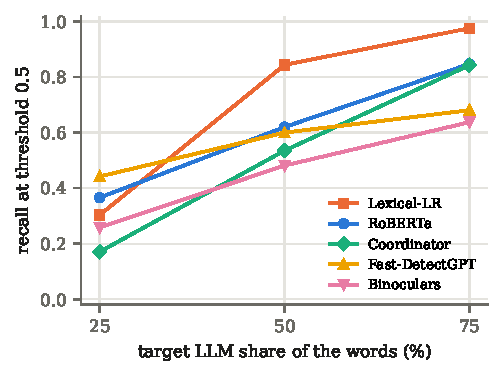
\includegraphics[width=\columnwidth]{mix_recall.pdf}
\caption{CISA + ABC ile eğitilen modellerde, kısmen üretilmiş metinlerde duyarlılığın LLM kelime payına göre
değişimi.}
\label{fig:mix}
\end{figure}

\begin{table*}[t]
\centering
\footnotesize
\caption{Eşik 0.5'te duyarlılık (üç seed üzerinden ortalama $\pm$ std): ABC ile eğitim (temel) ve ABC'ye eğitim kaynaklarının tek ajanlı ve yeniden ifade edilmiş metinleri eklenerek eğitim (art.).}
\label{tab:augmented}
\begin{tabular}{lcccccc}
\toprule
Test & \multicolumn{2}{c}{Lexical-LR} & \multicolumn{2}{c}{RoBERTa} & \multicolumn{2}{c}{Koordinatör} \\
 & temel & art. & temel & art. & temel & art. \\
\midrule
A & 0.996$\pm$0.007 & 0.996$\pm$0.007 & 1.000$\pm$0.000 & 1.000$\pm$0.000 & 1.000$\pm$0.000 & 1.000$\pm$0.000 \\
D & 0.801$\pm$0.018 & 0.969$\pm$0.028 & 0.958$\pm$0.030 & 0.995$\pm$0.008 & 0.851$\pm$0.046 & 0.866$\pm$0.087 \\
E & 1.000$\pm$0.000 & 1.000$\pm$0.000 & 1.000$\pm$0.000 & 1.000$\pm$0.000 & 1.000$\pm$0.000 & 1.000$\pm$0.000 \\
Yeniden ifade, aynı model & 0.999$\pm$0.002 & 1.000$\pm$0.000 & 1.000$\pm$0.000 & 1.000$\pm$0.000 & 1.000$\pm$0.000 & 1.000$\pm$0.000 \\
İki kez yeniden ifade & 1.000$\pm$0.000 & 1.000$\pm$0.000 & 1.000$\pm$0.000 & 1.000$\pm$0.000 & 1.000$\pm$0.000 & 1.000$\pm$0.000 \\
``İnsanlaştır'' promptu & 0.999$\pm$0.002 & 1.000$\pm$0.000 & 1.000$\pm$0.000 & 0.999$\pm$0.002 & 0.999$\pm$0.002 & 0.999$\pm$0.002 \\
Tek ajan & 0.663$\pm$0.113 & 0.892$\pm$0.051 & 0.721$\pm$0.052 & 0.976$\pm$0.009 & 0.601$\pm$0.121 & 0.766$\pm$0.119 \\
\bottomrule
\end{tabular}
\end{table*}

Bu koşullarla eğitim, temel modellerin başarısız olduğu yerde yardımcı oluyor (Tablo~\ref{tab:augmented}). Eğitim
kaynaklarının yeniden ifade edilmiş ve tek ajanlı metinlerini eklemek, tek ajanlı test metinlerindeki duyarlılığı
Lexical-LR'de \AugMainSingleLexlr{} değerinden \AugAugRewriteSingleLexlr{} değerine, RoBERTa'da
\AugMainSingleTrans{} değerinden \AugAugRewriteSingleTrans{} değerine çıkarıyor. Hiç D metni eklenmediği hâlde
D'deki duyarlılık da \AugMainDLexlr{} değerinden \AugAugRewriteDLexlr{} değerine ve \AugMainDTrans{} değerinden
\AugAugRewriteDTrans{} değerine yükseliyor. Koordinatör daha az kazanıyor (tek ajanlı metinlerde
\AugMainSingleCoord{} değerinden \AugAugRewriteSingleCoord{} değerine).

\begin{table*}[t]
\centering
\scriptsize\setlength{\tabcolsep}{2.5pt}
\caption{Test verisinde olasılık kalitesi, A, B veya C'den biriyle eğitim (üç seed üzerinden ortalama $\pm$ std). Kalibratörler yalnızca doğrulama verisiyle kurulur.}
\label{tab:calibration}
\begin{tabular}{@{}ll@{\ }ccccccccc@{}}
\toprule
Dedektör & Kalibratör & \multicolumn{3}{c}{Aynı üretici} & \multicolumn{3}{c}{D: gpt-oss-120b} & \multicolumn{3}{c}{E: Gemini} \\
 & & Brier & ECE & NLL & Brier & ECE & NLL & Brier & ECE & NLL \\
\midrule
Lexical-LR & Ham & 0.036$\pm$0.002 & 0.170$\pm$0.004 & 0.194$\pm$0.005 & 0.201$\pm$0.007 & 0.311$\pm$0.012 & 0.571$\pm$0.015 & 0.074$\pm$0.004 & 0.245$\pm$0.007 & 0.296$\pm$0.010 \\
Lexical-LR & Platt & 0.002$\pm$0.002 & 0.004$\pm$0.002 & 0.014$\pm$0.018 & 0.269$\pm$0.084 & 0.297$\pm$0.083 & 1.822$\pm$0.363 & 0.015$\pm$0.016 & 0.027$\pm$0.018 & 0.056$\pm$0.056 \\
Lexical-LR & Sıcaklık & 0.003$\pm$0.004 & 0.008$\pm$0.007 & 0.027$\pm$0.034 & 0.348$\pm$0.062 & 0.377$\pm$0.034 & 2.892$\pm$1.756 & 0.030$\pm$0.009 & 0.051$\pm$0.014 & 0.139$\pm$0.054 \\
Lexical-LR & İzotonik & 0.003$\pm$0.002 & 0.007$\pm$0.002 & 0.018$\pm$0.020 & 0.241$\pm$0.057 & 0.287$\pm$0.065 & 2.050$\pm$0.526 & 0.015$\pm$0.013 & 0.036$\pm$0.022 & 0.058$\pm$0.050 \\
RoBERTa & Ham & 0.007$\pm$0.001 & 0.015$\pm$0.002 & 0.032$\pm$0.005 & 0.104$\pm$0.032 & 0.120$\pm$0.032 & 0.406$\pm$0.133 & 0.010$\pm$0.004 & 0.018$\pm$0.004 & 0.039$\pm$0.018 \\
RoBERTa & Platt & 0.007$\pm$0.002 & 0.010$\pm$0.003 & 0.037$\pm$0.002 & 0.178$\pm$0.068 & 0.190$\pm$0.070 & 1.755$\pm$1.064 & 0.019$\pm$0.015 & 0.024$\pm$0.014 & 0.128$\pm$0.128 \\
RoBERTa & Sıcaklık & 0.008$\pm$0.001 & 0.013$\pm$0.005 & 0.044$\pm$0.020 & 0.111$\pm$0.038 & 0.122$\pm$0.032 & 0.832$\pm$0.562 & 0.010$\pm$0.004 & 0.018$\pm$0.006 & 0.062$\pm$0.026 \\
RoBERTa & İzotonik & 0.006$\pm$0.002 & 0.008$\pm$0.003 & 0.042$\pm$0.019 & 0.168$\pm$0.065 & 0.192$\pm$0.068 & 1.746$\pm$1.272 & 0.016$\pm$0.012 & 0.022$\pm$0.014 & 0.131$\pm$0.156 \\
Koordinatör & Ham & 0.002$\pm$0.001 & 0.006$\pm$0.000 & 0.009$\pm$0.002 & 0.161$\pm$0.048 & 0.209$\pm$0.048 & 0.594$\pm$0.210 & 0.007$\pm$0.007 & 0.023$\pm$0.010 & 0.031$\pm$0.020 \\
Koordinatör & Platt & 0.003$\pm$0.001 & 0.005$\pm$0.002 & 0.023$\pm$0.012 & 0.180$\pm$0.051 & 0.202$\pm$0.045 & 1.374$\pm$0.458 & 0.007$\pm$0.006 & 0.013$\pm$0.005 & 0.035$\pm$0.019 \\
Koordinatör & Sıcaklık & 0.004$\pm$0.001 & 0.005$\pm$0.002 & 0.033$\pm$0.018 & 0.191$\pm$0.058 & 0.203$\pm$0.051 & 2.124$\pm$0.790 & 0.008$\pm$0.008 & 0.013$\pm$0.008 & 0.059$\pm$0.053 \\
Koordinatör & İzotonik & 0.003$\pm$0.000 & 0.006$\pm$0.002 & 0.026$\pm$0.014 & 0.172$\pm$0.045 & 0.206$\pm$0.050 & 1.450$\pm$0.405 & 0.007$\pm$0.005 & 0.015$\pm$0.006 & 0.038$\pm$0.024 \\
\bottomrule
\end{tabular}
\end{table*}

\begin{table*}[t]
\centering
\footnotesize
\caption{Karar kuralının etkisi, A, B veya C'den biriyle eğitim. Bütün eşikler doğrulama verisinde belirlenir. Sözde görülmemiş kural, ne eğitimde ne de testte bulunan yerel üreticilerin doğrulama metinlerini kullanır. İnsan \%1 ve \%5 kuralları yalnızca doğrulama insan skorlarını kullanır.}
\label{tab:thresholds}
\begin{tabular}{llccccccc}
\toprule
Dedektör & Eşik kuralı & F1, aynı & F1, çapraz & F1, D & Duyarlılık, D & F1, E & F1, dış & FPR, dış \\
\midrule
Lexical-LR & Sabit 0.5 & 0.997$\pm$0.004 & 0.966$\pm$0.009 & 0.336$\pm$0.032 & 0.213 & 0.960$\pm$0.013 & 0.982$\pm$0.001 & 0.004 \\
Lexical-LR & Doğrulama F1 & 0.997$\pm$0.003 & 0.977$\pm$0.021 & 0.510$\pm$0.113 & 0.373 & 0.980$\pm$0.023 & 0.982$\pm$0.006 & 0.017 \\
Lexical-LR & Sözde görülmemiş F1 & 0.996$\pm$0.004 & 0.994$\pm$0.002 & 0.752$\pm$0.061 & 0.613 & 0.996$\pm$0.004 & 0.973$\pm$0.003 & 0.054 \\
Lexical-LR & İnsan \%5 FPR & 0.986$\pm$0.020 & 0.985$\pm$0.019 & 0.869$\pm$0.014 & 0.797 & 0.986$\pm$0.020 & 0.914$\pm$0.025 & 0.189 \\
Lexical-LR & İnsan \%1 FPR & 0.991$\pm$0.013 & 0.991$\pm$0.013 & 0.849$\pm$0.025 & 0.754 & 0.991$\pm$0.013 & 0.936$\pm$0.029 & 0.137 \\
RoBERTa & Sabit 0.5 & 0.991$\pm$0.002 & 0.989$\pm$0.002 & 0.845$\pm$0.061 & 0.770 & 0.988$\pm$0.005 & 0.953$\pm$0.011 & 0.099 \\
RoBERTa & Doğrulama F1 & 0.992$\pm$0.002 & 0.989$\pm$0.002 & 0.771$\pm$0.108 & 0.675 & 0.984$\pm$0.014 & 0.964$\pm$0.010 & 0.071 \\
RoBERTa & Sözde görülmemiş F1 & 0.988$\pm$0.005 & 0.987$\pm$0.002 & 0.801$\pm$0.134 & 0.722 & 0.980$\pm$0.013 & 0.965$\pm$0.009 & 0.070 \\
RoBERTa & İnsan \%5 FPR & 0.975$\pm$0.006 & 0.975$\pm$0.006 & 0.939$\pm$0.027 & 0.929 & 0.975$\pm$0.007 & 0.908$\pm$0.006 & 0.203 \\
RoBERTa & İnsan \%1 FPR & 0.989$\pm$0.008 & 0.987$\pm$0.007 & 0.860$\pm$0.106 & 0.788 & 0.984$\pm$0.007 & 0.953$\pm$0.018 & 0.099 \\
Koordinatör & Sabit 0.5 & 0.996$\pm$0.001 & 0.993$\pm$0.005 & 0.732$\pm$0.089 & 0.605 & 0.993$\pm$0.010 & 0.990$\pm$0.002 & 0.015 \\
Koordinatör & Doğrulama F1 & 0.996$\pm$0.001 & 0.992$\pm$0.005 & 0.719$\pm$0.051 & 0.586 & 0.992$\pm$0.009 & 0.991$\pm$0.000 & 0.014 \\
Koordinatör & Sözde görülmemiş F1 & 0.994$\pm$0.002 & 0.992$\pm$0.003 & 0.807$\pm$0.140 & 0.713 & 0.990$\pm$0.007 & 0.981$\pm$0.009 & 0.038 \\
Koordinatör & İnsan \%5 FPR & 0.981$\pm$0.011 & 0.981$\pm$0.010 & 0.949$\pm$0.013 & 0.938 & 0.981$\pm$0.011 & 0.929$\pm$0.006 & 0.154 \\
Koordinatör & İnsan \%1 FPR & 0.993$\pm$0.004 & 0.993$\pm$0.004 & 0.910$\pm$0.021 & 0.851 & 0.993$\pm$0.004 & 0.956$\pm$0.017 & 0.092 \\
\bottomrule
\end{tabular}
\end{table*}

\subsection{Kalibrasyon ve karar eşikleri}
Aynı üreticide doğrulama verisiyle kalibrasyon olasılıkları iyileştiriyor. Lexical-LR'nin beklenen kalibrasyon
hatası ham hâlde \CalLexlrRawInEce{} iken Platt ölçeklemeyle \CalLexlrPlattInEce{} oluyor
(Tablo~\ref{tab:calibration}). Üretici kayması altında ise olasılıklar kötüleşiyor. D'de Lexical-LR'nin negatif
log-olabilirliği \CalLexlrRawDNll{} (ham) değerinden \CalLexlrPlattDNll{} (Platt) ve \CalLexlrIsotonicDNll{}
(izotonik) değerlerine, RoBERTa'nınki \CalTransRawDNll{} değerinden \CalTransPlattDNll{} ve
\CalTransIsotonicDNll{} değerlerine çıkıyor. Kalibratörler doğrulama verisinden skorların güvenilir olduğunu
öğrenip onları keskinleştiriyor; D'de keskinleşen skorlar yanlış (Şekil~\ref{fig:reliability}). Bütün skorları
ancak birlikte yumuşatıp keskinleştirebilen sıcaklık ölçekleme RoBERTa'ya en az zarar veren yöntem (NLL
\CalTransTemperatureDNll{}). 0.5 eşiğindeki kararlara etkisi ise karışık. Platt ölçekleme Lexical-LR'nin sınırını
D'deki F1 değerini \CalfoneLexlrRawD{} düzeyinden \CalfoneLexlrPlattD{} düzeyine çıkaracak kadar kaydırıyor,
RoBERTa'nınkini ise \CalfoneTransRawD{} düzeyinden \CalfoneTransPlattD{} düzeyine indiriyor. Dağılım içi veriyle
kalibrasyon karar için güvenilir bir onarım değil, olasılıklar için de güvenli değil.

\begin{figure*}[t]
\centering
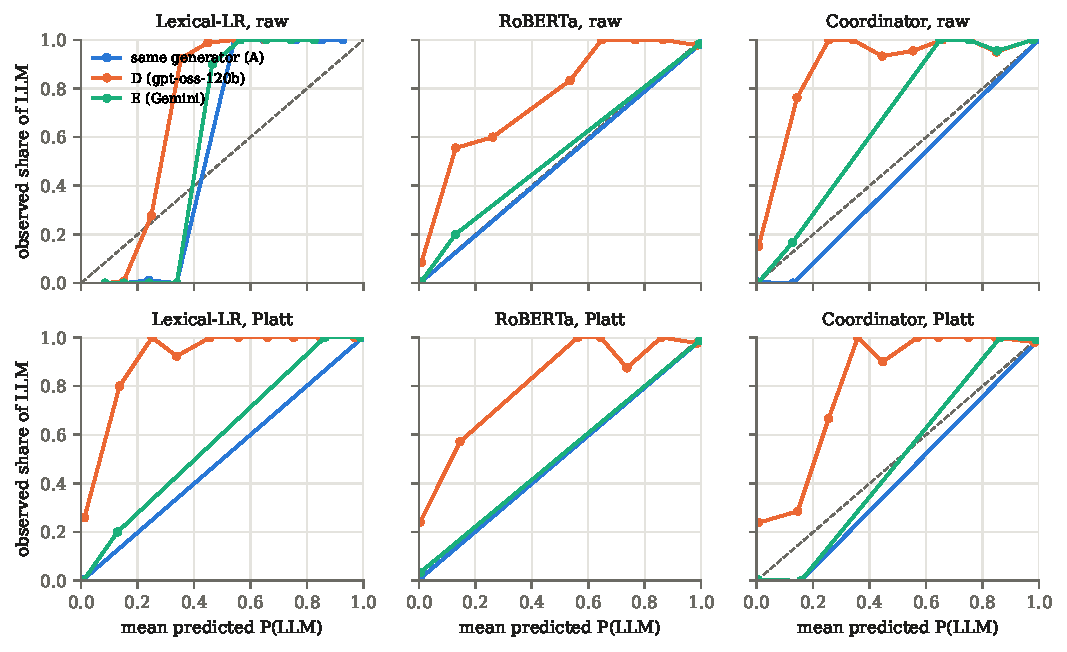
\includegraphics[width=0.9\textwidth]{reliability.pdf}
\caption{A ile eğitilen modellerde ham (üst) ve Platt ölçeklenmiş (alt) olasılıkların güvenilirliği. Noktalar en az
beş metin içeren kutular; kesikli köşegen kusursuz kalibrasyon.}
\label{fig:reliability}
\end{figure*}

Eşik, kalibratörden daha önemli (Tablo~\ref{tab:thresholds}, Şekil~\ref{fig:sweep}). Doğrulama F1 değerini en
yükseğe çıkaran eşiği seçmek güvenilir bir çözüm değil, çünkü doğrulama metinleri eğitim üreticisinden geliyor. Bu
kural Lexical-LR'yi D'de ancak \ThrDLexlrValfFOne{} düzeyine çıkarıyor, RoBERTa'yı \ThrDTransValfFOne{} düzeyine
düşürüyor. Eşiği başka bir yerel üreticide ayarlayan sözde görülmemiş kural, Lexical-LR'nin D'deki F1 değerini
\ThrDLexlrFixedFOne{} düzeyinden \ThrDLexlrPseudoFOne{} düzeyine çıkarıyor. Hiç LLM metni kullanmayan iki insan
yüzdeliği kuralı bu değeri \ThrDLexlrHumoneFOne{} (\%1 hedefi) ve \ThrDLexlrHumfiveFOne{} (\%5 hedefi) düzeyine,
Koordinatör'ünkini \ThrDCoordFixedFOne{} düzeyinden \ThrDCoordHumoneFOne{} ve \ThrDCoordHumfiveFOne{} düzeyine
çıkarıyor. D skorlarının çoğu zaten 0.5'in üstünde olan RoBERTa daha az kazanıyor (\ThrDTransFixedFOne{}
düzeyinden \ThrDTransHumfiveFOne{} düzeyine).

Bedeli diğer yayıncılarda görülüyor. Tablo~\ref{tab:thresholds} tek üreticiyle eğitilen modeller için hesaplandı.
Bu modeller sabit eşikte firma parçalarının yalnızca \ThrExternalLexlrFixedFpr{} (Lexical-LR) ve
\ThrExternalCoordFixedFpr{} (Koordinatör) kadarını işaretliyor, yani Tablo~\ref{tab:publishers}'teki havuzlanmış
modellerden çok daha azını. \%5 kuralıyla bu oranlar \ThrExternalLexlrHumfiveFpr{} ve
\ThrExternalCoordHumfiveFpr{} oluyor. Firma insan metinleri CISA metinlerinden yüksek skor aldığı için CISA
skorlarının bir yüzdeliği bunların daha çoğunu geçiriyor. Beş kuraldan D'yi en çok geri kazandıranlar, firma
metinlerinde yanlış alarmı da en çok artıranlar. Havuzlanmış eğitimde gördüğümüz bedelin aynısı.

\begin{figure}[t]
\centering
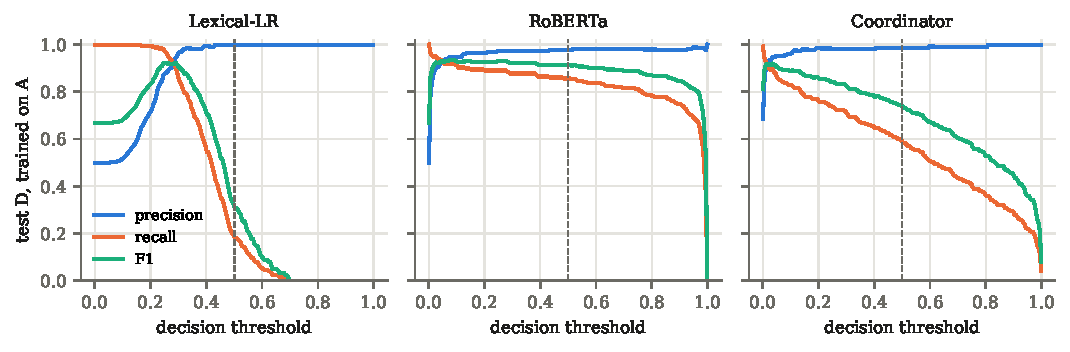
\includegraphics[width=\columnwidth]{threshold_sweep.pdf}
\caption{A ile eğitilen modellerde D üzerinde kesinlik, duyarlılık ve F1'in karar eşiğine göre değişimi; kesikli
çizgi 0.5.}
\label{fig:sweep}
\end{figure}

\begin{table*}[t]
\centering
\footnotesize\setlength{\tabcolsep}{3pt}
\caption{Bütün senaryolarda eşik 0.5'te RoBERTa, Koordinatör ve türevlerinin F1 değeri (çalıştırmalar üzerinden ortalama; ilk ikisinde seed'ler üzerinden $\pm$ std). Fark, Koordinatör eksi RoBERTa; aralık kaynak düzeyinde eşleştirilmiş bootstrap ile; * Holm düzeltmeli p $<$ 0.05. ``Görülmemiş yığın'' Koordinatör'ü eğitimde olmayan üreticilerin doğrulama metinleriyle kurar. ``Çok ajan, aynı kaynaklar'' tek ajan satırının referansıdır.}
\label{tab:coordinator}
\begin{tabular}{@{}lcccccccc@{}}
\toprule
Senaryo & RoBERTa & Koord. & Fark & \%95 GA & Doğr. en iyi & Ort. logit & Görülm. yığın & + sıfır örn. \\
\midrule
Aynı üretici & 0.991$\pm$0.002 & 0.996$\pm$0.001 & +0.005* & [+0.001, +0.010] & 0.997 & 0.998 & 0.997 & 0.996 \\
Çapraz, yerel & 0.989$\pm$0.002 & 0.993$\pm$0.005 & +0.004 & [+0.000, +0.008] & 0.973 & 0.994 & 0.994 & 0.992 \\
Birini dışarıda bırak & 0.975$\pm$0.006 & 0.994$\pm$0.002 & +0.018* & [+0.011, +0.026] & 0.991 & 0.995 & -- & 0.994 \\
D, tek üretici & 0.845$\pm$0.061 & 0.732$\pm$0.089 & -0.113* & [-0.137, -0.089] & 0.388 & 0.747 & 0.811 & 0.736 \\
D, ABC & 0.947$\pm$0.020 & 0.922$\pm$0.048 & -0.024 & [-0.052, +0.002] & 0.796 & 0.965 & -- & 0.920 \\
E, tek üretici & 0.988$\pm$0.005 & 0.993$\pm$0.010 & +0.005 & [-0.001, +0.010] & 0.966 & 0.997 & 0.996 & 0.991 \\
E, ABC & 0.973$\pm$0.015 & 0.998$\pm$0.004 & +0.024* & [+0.011, +0.039] & 0.989 & 0.996 & -- & 0.998 \\
Microsoft, ABC & 0.909$\pm$0.046 & 0.978$\pm$0.010 & +0.069* & [+0.063, +0.075] & 0.952 & 0.954 & -- & 0.981 \\
Mandiant, ABC & 0.901$\pm$0.054 & 0.970$\pm$0.016 & +0.069* & [+0.062, +0.076] & 0.958 & 0.935 & -- & 0.972 \\
Yalnız Yazar, ABC & 0.973$\pm$0.015 & 0.998$\pm$0.004 & +0.024* & [+0.017, +0.033] & 0.989 & 0.996 & -- & 0.998 \\
Yeniden ifade, ABC & 0.973$\pm$0.015 & 0.998$\pm$0.004 & +0.025* & [+0.017, +0.032] & 0.988 & 0.996 & -- & 0.998 \\
Yeniden ifade, başka model, ABC & 0.973$\pm$0.015 & 0.998$\pm$0.004 & +0.024* & [+0.017, +0.032] & 0.988 & 0.996 & -- & 0.998 \\
İki kez yeniden ifade, ABC & 0.973$\pm$0.015 & 0.998$\pm$0.004 & +0.025* & [+0.017, +0.032] & 0.988 & 0.996 & -- & 0.998 \\
Geri çeviri, ABC & 0.968$\pm$0.014 & 0.995$\pm$0.005 & +0.027* & [+0.020, +0.036] & 0.987 & 0.995 & -- & 0.995 \\
``İnsanlaştır'' promptu, ABC & 0.973$\pm$0.016 & 0.997$\pm$0.003 & +0.024* & [+0.017, +0.033] & 0.989 & 0.996 & -- & 0.997 \\
Bildiri üslubu promptu, ABC & 0.974$\pm$0.014 & 0.998$\pm$0.004 & +0.024* & [+0.016, +0.032] & 0.987 & 0.995 & -- & 0.998 \\
Az örnekli prompt, ABC & 0.959$\pm$0.018 & 0.973$\pm$0.005 & +0.014* & [+0.004, +0.024] & 0.969 & 0.979 & -- & 0.974 \\
Çok ajan, aynı kaynaklar, ABC & 0.994$\pm$0.010 & 1.000$\pm$0.000 & +0.006 & [+0.000, +0.012] & 0.994 & 1.000 & -- & 1.000 \\
Tek ajan, ABC & 0.816$\pm$0.084 & 0.694$\pm$0.137 & -0.122* & [-0.168, -0.082] & 0.694 & 0.764 & -- & 0.700 \\
\%25 LLM, ABC & 0.574$\pm$0.065 & 0.274$\pm$0.044 & -0.300* & [-0.341, -0.261] & 0.356 & 0.408 & -- & 0.271 \\
\%50 LLM, ABC & 0.770$\pm$0.043 & 0.705$\pm$0.057 & -0.064* & [-0.088, -0.043] & 0.730 & 0.790 & -- & 0.708 \\
\%75 LLM, ABC & 0.906$\pm$0.003 & 0.920$\pm$0.007 & +0.014 & [+0.001, +0.027] & 0.926 & 0.949 & -- & 0.921 \\
\bottomrule
\end{tabular}
\end{table*}

\subsection{Koordinatör ne zaman yardımcı oluyor}
Tablo~\ref{tab:coordinator} Koordinatör'ü \GapN{} senaryonun hepsinde RoBERTa ile karşılaştırıyor. Referans RoBERTa,
çünkü kayma altında en az kaybeden üye o. Aynı üreticide Lexical-SVM de Koordinatör kadar iyi
(Tablo~\ref{tab:main}). Koordinatör \GapWins{} senaryoda RoBERTa'dan iyi, \GapLosses{} senaryoda kötü (Holm
düzeltmeli $p<0.05$). İkisinin de tavana yakın olduğu yerlerde kazanç küçük (aynı üretici \GapInGenerator{}, birini
dışarıda bırak \GapLeaveOneOut{}, yeniden ifade koşulları). Daha düşük yanlış pozitif oranının işe yaradığı firma
metinlerinde daha büyük (Microsoft \GapMicrosoftAbc{}, Mandiant \GapMandiantAbc{}). Kayıplar kanıtı en çok
değiştiren kaymalarda: kelimelerinin dörtte biri LLM'den gelen metinler (\GapTwoFiveLlmAbc{}), tek üreticiyle
eğitimden sonra D (\GapDOneGenerator{}, \%95 GA [\GapLoDOneGenerator{}, \GapHiDOneGenerator{}]), tek ajanlı metinler
(\GapSingleAgentAbc{}), yarısı LLM'den gelen metinler (\GapFiveZeroLlmAbc{}) ve üç üreticiyle eğitimden sonra D
(\GapDAbc{}).

Doğrulama verisinde yığın en çok Lexical-SVM (\WgtLexsvm{}) ve RoBERTa'ya (\WgtTrans{}), sonra Stilometri
(\WgtStylo{}) ve Lexical-LR'ye (\WgtLexlr{}) ağırlık veriyor. LLM Yargıç negatif ağırlık alıyor (\WgtJudge{}). D'de
Lexical-SVM'in ortalama logiti çöküyor. Katsayısıyla ağırlıklandırıldığında Koordinatör'ün düşüşünün
\DropLexsvm{} logit birimini açıklıyor. RoBERTa'nın payı \DropTrans{}, Stilometri'ninki \DropStylo{}. Eğitim
üreticisinde kurulan ağırlıklar yani en çok güveni D'de başarısız olan bir üyeye veriyor. Doğrulamada en iyi tek
üyeyi seçmek daha kötü sonuç veriyor (D'de F1 \ScDOneGeneratorBestVal{}; en sık seçilen üye \BestValTop{}),
logitlerin ağırlıksız ortalaması biraz daha iyi (\ScDOneGeneratorCoordMean{}), eğitimde bulunmayan yerel
üreticilerin doğrulama metinleriyle kurulan yığın en iyisi (\ScDOneGeneratorCoordUnseen{}). Hiçbiri tek başına
RoBERTa'ya (\ScDOneGeneratorTrans{}) ulaşamıyor. İki sıfır örnekli dedektörü üye olarak eklemek pek bir şey
değiştirmiyor (\ScDOneGeneratorCoordZero{}). RoBERTa'yı Koordinatör'den çıkarmak D'deki F1 değerini
\CoordNoTransD{} düzeyine düşürüyor. Başka herhangi bir üyeyi çıkarmak en çok \CoordDropMaxOther{} değiştiriyor
(Tablo~\ref{tab:ablation}).

\begin{table*}[t]
\centering
\footnotesize
\caption{Ablasyonlar, F1 (seed'ler üzerinden ortalama $\pm$ std; A, B veya C'den biriyle eğitim).}
\label{tab:ablation}
\begin{tabular}{lcccc}
\toprule
Koşul & Aynı üretici & Çapraz (A--C) & D & E \\
\midrule
Yalnız TF-IDF (LR) & 0.997 $\pm$ 0.004 & 0.966 $\pm$ 0.008 & 0.329 $\pm$ 0.017 & 0.961 $\pm$ 0.012 \\
Yalnız stilometri (XGB) & 0.934 $\pm$ 0.006 & 0.868 $\pm$ 0.004 & 0.706 $\pm$ 0.013 & 0.778 $\pm$ 0.022 \\
TF-IDF + stilometri (LR) & 0.964 $\pm$ 0.005 & 0.919 $\pm$ 0.010 & 0.735 $\pm$ 0.060 & 0.839 $\pm$ 0.021 \\
LR, çıktı temizliği kapalı & 0.997 $\pm$ 0.004 & 0.965 $\pm$ 0.008 & 0.336 $\pm$ 0.018 & 0.955 $\pm$ 0.012 \\
LR, kurum adları maskeli & 0.996 $\pm$ 0.004 & 0.967 $\pm$ 0.008 & 0.349 $\pm$ 0.016 & 0.964 $\pm$ 0.012 \\
RoBERTa, kurum adları maskeli & 0.988 $\pm$ 0.004 & 0.986 $\pm$ 0.002 & 0.901 $\pm$ 0.035 & 0.985 $\pm$ 0.007 \\
Stilometri: yalnız uzunluk & 0.875 $\pm$ 0.008 & 0.790 $\pm$ 0.004 & 0.482 $\pm$ 0.060 & 0.657 $\pm$ 0.039 \\
Stilometri: yalnız sözcük çeşitliliği & 0.845 $\pm$ 0.025 & 0.816 $\pm$ 0.024 & 0.863 $\pm$ 0.025 & 0.865 $\pm$ 0.033 \\
Stilometri: yalnız noktalama & 0.823 $\pm$ 0.012 & 0.771 $\pm$ 0.024 & 0.492 $\pm$ 0.055 & 0.590 $\pm$ 0.043 \\
Stilometri: yalnız tekrar & 0.800 $\pm$ 0.020 & 0.769 $\pm$ 0.024 & 0.825 $\pm$ 0.020 & 0.775 $\pm$ 0.037 \\
Stilometri: yalnız POS & 0.814 $\pm$ 0.038 & 0.755 $\pm$ 0.036 & 0.777 $\pm$ 0.052 & 0.850 $\pm$ 0.063 \\
Koordinatör, tüm ajanlar & 0.998 $\pm$ 0.000 & 0.993 $\pm$ 0.003 & 0.721 $\pm$ 0.083 & 0.995 $\pm$ 0.003 \\
Koordinatör, Lexical-LR olmadan & 0.998 $\pm$ 0.000 & 0.993 $\pm$ 0.003 & 0.727 $\pm$ 0.084 & 0.995 $\pm$ 0.003 \\
Koordinatör, Lexical-SVM olmadan & 0.996 $\pm$ 0.002 & 0.990 $\pm$ 0.008 & 0.784 $\pm$ 0.058 & 0.991 $\pm$ 0.002 \\
Koordinatör, LLM Yargıç olmadan & 0.999 $\pm$ 0.001 & 0.993 $\pm$ 0.004 & 0.732 $\pm$ 0.102 & 0.996 $\pm$ 0.004 \\
Koordinatör, Stilometri olmadan & 0.998 $\pm$ 0.002 & 0.994 $\pm$ 0.001 & 0.722 $\pm$ 0.125 & 0.992 $\pm$ 0.004 \\
Koordinatör, RoBERTa olmadan & 0.997 $\pm$ 0.003 & 0.972 $\pm$ 0.007 & 0.490 $\pm$ 0.094 & 0.960 $\pm$ 0.006 \\
\bottomrule
\end{tabular}
\end{table*}

\subsection{Ablasyonlar}
Kurum adlarını maskelemek Lexical-LR'yi neredeyse hiç değiştirmiyor (aynı üreticide \AblLrMaskedIn{}, üreticiler
arası \AblLrMaskedCross{}); \emph{CISA} kelimesi log-odds listesinin başında olsa da dedektörler ona bağlı değil.
Çıktı temizliğini kapatmak bir şey değiştirmiyor (\AblLrNoCleanIn{}).

Uzunluğu eşleştirilmiş alt küme, uzunluğu insan parçasının \%20 yakınında kalan LLM metinlerini tutuyor. A üreticisi
neredeyse hiç bu kadar uzun yazmıyor (test kümesi başına yaklaşık \LenAN{} metin). Bu yüzden test kümesi başına
\LenBN{} ve \LenCN{} metin bulunan B ve C'yi veriyoruz. Sözcüksel dedektörler ve RoBERTa etkilenmiyor (Lexical-LR
\LenBLexLR{} ve \LenCLexLR{}, RoBERTa \LenBTrans{} ve \LenCTrans{}). Stilometri B'de \SameBStylo{} düzeyinden
\LenBStylo{} düzeyine, C'de \SameCStylo{} düzeyinden \LenCStylo{} düzeyine düşüyor. Demek ki kısa yazan üreticilerde
stilometrik sinyalin bir kısmını uzunluk taşıyor. Bu en açık B'de görülüyor ve alt kümeler küçük. Özellik grupları
aynı cevabı daha büyük bir örnekte veriyor. Uzunluk ve noktalama özellikleri aynı üreticide \AblGroupLengthIn{} ve
\AblGroupPunctuationIn{} veriyor, ama insan uzunluğunu tutturan D'de \AblGroupLengthD{} ve
\AblGroupPunctuationD{}. Tek başına sözcük çeşitliliği ise D'de \AblGroupLexicalD{} veriyor. Bu, tam stilometrik
modelin verdiğinden (\AblStylometryD{}) yüksek.

Bir Yazar şablonunu eğitimin dışında tutmak, Lexical-LR'nin o şablondaki duyarlılığını şablona göre
\TplRecallMin{} ile \TplRecallMax{} arasına düşürüyor; AUC değeri ise \TplAucMin{} olarak kalıyor. Metinleri
sıralamak için tek bir şablona gerek yok, ama sabit eşikte şablonlar birbirinin yerine geçmiyor. Koordinatör'ün
diğer yerel üreticilerdeki duyarlılığı konuya göre \TopicCrossMin{} ile \TopicCrossMax{} arasında. D'de en düşük
duyarlılık zafiyet ve APT raporlarında (\TopicDVulnerability{} ve \TopicDApt{}), en yüksek duyarlılık küçük
``diğer'' grubunda (\TopicDOther{}).

\begin{table*}[t]
\centering
\footnotesize
\caption{Maliyet ve başarım, tek eğitim üreticisi. Çıkarım tek bir RTX 4060 dizüstü GPU'da, sabit bir örnek üzerinde üç tekrar. Koordinatör'ün maliyeti üyelerinin art arda çalışma süresinin toplamıdır; ``Eğitim'' sütunu eğitilmeyen LLM Yargıç'ı içermez.}
\label{tab:cost}
\begin{tabular}{lrrrrcccc}
\toprule
Dedektör & ms/metin & Oran & GPU MiB & Eğitim s & F1, aynı & F1, D & AUC, D & F1, E \\
\midrule
Lexical-LR & 1.7 & 0.60 & -- & 1 & 0.997 & 0.329 & 0.979 & 0.961 \\
Lexical-SVM & 2.0 & 0.72 & -- & 1 & 0.998 & 0.327 & 0.983 & 0.969 \\
Stilometri & 25.6 & 9.27 & -- & 0 & 0.934 & 0.706 & 0.878 & 0.778 \\
RoBERTa & 2.8 & 1.00 & 1269 & 20 & 0.992 & 0.859 & 0.982 & 0.991 \\
LLM Yargıç & 1136.5 & 410.75 & 16 & -- & 0.504 & 0.499 & 0.533 & 0.628 \\
Fast-DetectGPT & 195.9 & 70.78 & 5771 & -- & 0.744 & 0.540 & 0.699 & 0.427 \\
Binoculars & 725.0 & 262.02 & 5005 & -- & 0.817 & 0.365 & 0.734 & 0.307 \\
Koordinatör & 1168.6 & 422.34 & -- & -- & 0.998 & 0.721 & 0.987 & 0.995 \\
\bottomrule
\end{tabular}
\end{table*}

\subsection{Maliyet}
Çıkarım maliyeti metin başına Lexical-LR'de \MsLexLR{}~ms ile LLM Yargıç'ta \MsJudge{}~ms arasında değişiyor
(Tablo~\ref{tab:cost}). RoBERTa GPU'da \MsTrans{}~ms, Fast-DetectGPT \MsFast{}~ms, Binoculars \MsBino{}~ms
istiyor. Üyeleri art arda çalıştırıldığında Koordinatör'ün maliyeti metin başına \MsCoord{}~ms ve neredeyse tamamı
Yargıç'tan geliyor. Yargıç olmadan \MsCoordNoJudge{}~ms. Yargıç'ın negatif yığın ağırlığı ve çıkarılmasının
sıfıra yakın etkisi, bu sürenin bizim verimizde karşılığının olmadığını gösteriyor.

\begin{table*}[t]
\centering
\footnotesize
\caption{Kaynağa göre ortalama metin özellikleri (A--E için çok ajanlı metinler). Birinci şahıs ve kurum adı: en az bir birinci şahıs zamiri veya kurum adı içeren metinlerin payı. İpuçları: Lexical-LR'nin iki yönde en büyük ağırlığı verdiği kelime n-gram'larının 100 kelimedeki geçiş sayısı (A ile eğitilen model).}
\label{tab:profile}
\begin{tabular}{lrrrrrrr}
\toprule
Kaynak & Kelime & MTLD & Özel ad & Birinci şahıs & Kurum adı & LLM yönlü ipucu & İnsan yönlü ipucu \\
\midrule
İnsan (CISA) & 279 & 86 & 0.118 & 14\% & 78\% & 0.77 & 5.45 \\
A: Llama 3.1 8B & 161 & 94 & 0.058 & 47\% & 10\% & 6.98 & 1.75 \\
B: Qwen 2.5 7B & 166 & 125 & 0.064 & 39\% & 11\% & 5.51 & 2.13 \\
C: Mistral 7B & 210 & 134 & 0.064 & 61\% & 17\% & 4.99 & 2.67 \\
D: gpt-oss-120b & 294 & 206 & 0.051 & 10\% & 13\% & 1.98 & 1.81 \\
E: Gemini 3.1 Flash-Lite & 279 & 170 & 0.035 & 45\% & 9\% & 3.44 & 1.46 \\
İnsan (Microsoft) & 312 & 95 & 0.063 & 77\% & 1\% & 1.37 & 2.26 \\
İnsan (Mandiant) & 295 & 93 & 0.078 & 74\% & 4\% & 1.62 & 2.38 \\
\bottomrule
\end{tabular}
\end{table*}

\begin{table*}[t]
\centering
\footnotesize
\caption{Bütün seed'ler üzerinden hata kategorileri: her dedektörün hatalarının sayısı ve payı. Kategoriler birbirini dışlar ve uyan ilk kurala göre atanır (Bölüm~\ref{sec:errors}); bir metin yanlış sınıflandırıldığı her çalıştırmada bir kez sayılır. ``Bütün metinler'', kategorinin gruptaki hatalı ya da hatasız bütün metinler içindeki payıdır; bir kategori ancak hatalar içindeki payı bunu aştığında hatalarda fazla temsil edilir. FN ve CISA satırları: tek üreticiyle eğitilen modeller; firma satırları: ABC ile eğitilen modeller.}
\label{tab:errors}
\begin{tabular}{llcccc}
\toprule
Hata & Kategori & Bütün metinler & Lexical-LR & RoBERTa & Koordinatör \\
\midrule
FN, D & kişisiz, insan uzunluğunda & 76\% & 429 (76\%) & 114 (72\%) & 211 (74\%) \\
FN, D & kurum adı geçiyor & 11\% & 60 (11\%) & 15 (9\%) & 28 (10\%) \\
FN, D & birinci şahıs, yine de kaçırıldı & 10\% & 44 (8\%) & 10 (6\%) & 22 (8\%) \\
FN, D & olgularda olmayan teknik ayrıntı & 4\% & 30 (5\%) & 19 (12\%) & 26 (9\%) \\
FN, diğer üreticiler & birinci şahıs, yine de kaçırıldı & 46\% & 44 (30\%) & 6 (46\%) & 11 (50\%) \\
FN, diğer üreticiler & kişisiz, kısa & 30\% & 43 (30\%) & 1 (8\%) & 2 (9\%) \\
FN, diğer üreticiler & kurum adı geçiyor & 7\% & 28 (19\%) & 5 (38\%) & 6 (27\%) \\
FN, diğer üreticiler & kişisiz, insan uzunluğunda & 17\% & 29 (20\%) & 1 (8\%) & 3 (14\%) \\
FN, diğer üreticiler & olgularda olmayan teknik ayrıntı & 0\% & 1 (1\%) & 0 & 0 \\
FP, CISA & birinci şahıs & 15\% & 0 & 3 (30\%) & 1 (50\%) \\
FP, CISA & ürün açığı bildirimi & 9\% & 0 & 3 (30\%) & 0 \\
FP, CISA & az özel ad & 19\% & 0 & 3 (30\%) & 0 \\
FP, CISA & diğer & 28\% & 0 & 1 (10\%) & 1 (50\%) \\
FP, firma blogları & birinci şahıs & 75\% & 170 (89\%) & 212 (91\%) & 61 (85\%) \\
FP, firma blogları & az özel ad & 16\% & 20 (11\%) & 19 (8\%) & 11 (15\%) \\
FP, firma blogları & ürün açığı bildirimi & 2\% & 0 & 2 (1\%) & 0 \\
\bottomrule
\end{tabular}
\end{table*}

\begin{table*}[t]
\centering
\footnotesize
\caption{Yanlış ve doğru sınıflandırılan metinlerin özellikleri: iki grubun ortalamaları ve Cliff $\delta$ değeri (yanlış sınıflandırılanlarda daha yüksekse pozitif). Bir metin, çalıştırmaların en az yarısında yanlış sınıflandırıldıysa ilk gruba girer. *, Benjamini-Hochberg düzeltmeli p $<$ 0.05 olan Mann-Whitney testini gösterir. D: tek üreticiyle eğitilen modeller; firma parçaları: ABC ile eğitilen modeller.}
\label{tab:contrast}
\begin{tabular}{llcccccc}
\toprule
Grup & Özellik & \multicolumn{2}{c}{Lexical-LR} & \multicolumn{2}{c}{RoBERTa} & \multicolumn{2}{c}{Koordinatör} \\
 & & ortalamalar & $\delta$ & ortalamalar & $\delta$ & ortalamalar & $\delta$ \\
\midrule
D, kaçan / yakalanan & Metin sayısı & 152 / 39 &  & 35 / 156 &  & 90 / 101 &  \\
 & Kelime & 301 / 258 & +0.32* & 322 / 285 & +0.25* & 331 / 258 & +0.52* \\
 & MTLD & 203 / 220 & -0.25* & 183 / 212 & -0.37* & 195 / 217 & -0.34* \\
 & Tür-örnek oranı (TTR) & 0.680 / 0.718 & -0.39* & 0.647 / 0.696 & -0.53* & 0.654 / 0.717 & -0.66* \\
 & Özel ad oranı & 0.055 / 0.038 & +0.36* & 0.052 / 0.052 & -0.02 & 0.061 / 0.043 & +0.35* \\
 & Birinci şahıslı metin payı & 0.08 / 0.18 & -0.10 & 0.06 / 0.11 & -0.05 & 0.09 / 0.11 & -0.02 \\
 & 100 kelimede LLM yönlü ipucu & 2.01 / 3.16 & -0.50* & 1.69 / 2.37 & -0.33* & 1.91 / 2.55 & -0.29* \\
 & 100 kelimede insan yönlü ipucu & 3.43 / 2.85 & +0.28* & 3.85 / 3.19 & +0.32* & 3.47 / 3.17 & +0.15 \\
 & Olgularda olmayan tanımlayıcı & 0.07 / 0.00 & +0.05 & 0.17 / 0.03 & +0.09* & 0.11 / 0.00 & +0.09* \\
Firma, işaretlenen / geçen & Metin sayısı & 64 / 374 &  & 79 / 359 &  & 15 / 423 &  \\
 & Kelime & 282 / 307 & -0.32* & 297 / 305 & -0.13 & 249 / 306 & -0.48* \\
 & MTLD & 108 / 92 & +0.39* & 109 / 91 & +0.43* & 121 / 93 & +0.64* \\
 & Tür-örnek oranı (TTR) & 0.587 / 0.556 & +0.42* & 0.588 / 0.554 & +0.38* & 0.635 / 0.558 & +0.76* \\
 & Özel ad oranı & 0.071 / 0.070 & +0.01 & 0.060 / 0.072 & -0.22* & 0.060 / 0.071 & -0.25 \\
 & Zamir oranı & 0.035 / 0.035 & +0.03 & 0.036 / 0.035 & +0.09 & 0.039 / 0.035 & +0.21 \\
 & 100 kelimede birinci şahıs & 1.47 / 0.86 & +0.35* & 1.44 / 0.84 & +0.38* & 1.19 / 0.94 & +0.14 \\
 & 100 kelimede LLM yönlü ipucu & 2.44 / 1.44 & +0.45* & 2.31 / 1.43 & +0.43* & 2.16 / 1.57 & +0.30 \\
 & 100 kelimede insan yönlü ipucu & 3.09 / 3.73 & -0.28* & 3.20 / 3.73 & -0.25* & 3.26 / 3.65 & -0.20 \\
\bottomrule
\end{tabular}
\end{table*}

\begin{table*}[t]
\centering
\footnotesize
\caption{Yüksek güvenle yapılan hatalara örnekler (CISA parçaları ve LLM çıktısı); üretici, uzunluk ve metni yanlış sınıflandıran çalıştırmalardaki ortalama skorla birlikte.}
\label{tab:examples}
\begin{tabular}{p{4.2cm}p{12.8cm}}
\toprule
Hata & Metnin başı \\
\midrule
FN, Koordinatör: olgularda olmayan teknik ayrıntı. Üretici D, 341 kelime, ortalama P(LLM) 0.00 & Malicious cyber actors have been observed deploying the KONNI malware family in campaigns that rely on a classic spear-phishing attachment workflow (ATT\&CK T1566.001). The initial infection vector typically consists of a malicious Microsoft Office document that contains a Visual Basic for Applications (VBA) macro. When the recipient enables macros, the VBA code executes a chain of actions designed to establish\ldots \\
FN, Koordinatör: kişisiz, insan uzunluğunda. Üretici D, 345 kelime, ortalama P(LLM) 0.07 & The investigation began after the security operations center received an alert that an administrative account in the organization's cloud-based email environment had been used to modify permissions and access a number of privileged mailboxes. Log correlation and forensic analysis quickly revealed activity consistent with tactics employed by Russian Federal Security Service (SVR) cyber-espionage groups. The adversary's foothold was established through\ldots \\
FN, Lexical-LR: kurum adı geçiyor. Üretici D, 317 kelime, ortalama P(LLM) 0.34 & Malicious cyber actors-most likely advanced persistent threat (APT) groups-have been observed exploiting a series of critical VMware vulnerabilities disclosed in early 2022, specifically CVE-2022-22954, CVE-2022-22960, CVE-2022-22972, and CVE-2022-22973. These flaws enable a server-side template injection (SSTI) that can be leveraged to achieve remote code execution (RCE) on affected VMware products and, in many cases, to elevate privileges to the root\ldots \\
FN, RoBERTa: birinci şahıs, yine de kaçırıldı. Üretici A, 122 kelime, ortalama P(LLM) 0.15 & Malicious cyber actors, likely advanced persistent threat (APT) actors, have been exploiting critical vulnerabilities affecting VMware products. The vulnerabilities, specifically CVE-2022-22954 and CVE-2022-22960, were addressed by VMware with updates on April 6, 2022. The US Cybersecurity and Infrastructure Security Agency (CISA) added these vulnerabilities to its catalog of Known Exploited Vulnerabilities on April 14 and 15, 2022, respectively. Federal agencies\ldots \\
FP, RoBERTa: birinci şahıs. CISA, 333 kelime, ortalama P(LLM) 0.61 & Since early 2018, we have observed an increase in JBiFrost RAT being used in targeted attacks against critical national infrastructure owners and their supply chain operators. There has also been an increase in the RAT's hosting on infrastructure located in our countries. In early 2017, Adwind RAT was deployed via spoofed emails designed to look as if they originated from\ldots \\
FP, RoBERTa: az özel ad. CISA, 309 kelime, ortalama P(LLM) 0.80 & The BeagleBoyz use a variety of tools and techniques to gain access to a financial institution's network, learn the topology to discover key systems, and monetize their access. The technical analysis below represents an amalgamation of multiple known incidents, rather than details of a single operation. These findings are presented to highlight the group's ability to tailor their techniques to\ldots \\
\bottomrule
\end{tabular}
\end{table*}

\subsection{Hata analizi}\label{sec:erranalysis}
\emph{Kategoriler ne gösteriyor.} Tablo~\ref{tab:errors} hata kategorilerini taban oranlarıyla birlikte veriyor.
Lexical-LR'nin kaçırdığı D metinlerinin \ErrFnDImpersonalHumanLengthLexlr{} kadarı kişisiz ve insan uzunluğunda.
Ama bütün D metinlerinin \ErrbaseFnDImpersonalHumanLength{} kadarı da öyle. Bu kategori D'nin nasıl yazdığını
anlatıyor, kaçanları ayırmıyor. Kurum adı geçen D metinleri için de durum aynı. Taban oranından ayrılan iki
kategori var. Birinci şahısla yazılmış D metinleri diğerlerinden daha az kaçıyor (Lexical-LR bunların
\ErrRateFnDFirstPersonStillMissedLexlr{} kadarını, kişisiz olanların \ErrRateFnDImpersonalHumanLengthLexlr{}
kadarını kaçırıyor). Analist olgularında bulunmayan teknik tanımlayıcılar içeren metinler ise daha çok kaçıyor.
Bunlar D metinlerinin \ErrbaseFnDUnsupportedTechnicalDetail{} kadarı, RoBERTa'nın kaçırdıklarının ise
\ErrFnDUnsupportedTechnicalDetailTrans{} kadarı; RoBERTa bunların \ErrRateFnDUnsupportedTechnicalDetailTrans{}
kadarını, kişisiz olanların \ErrRateFnDImpersonalHumanLengthTrans{} kadarını kaçırıyor. Bu grup küçük
(çalıştırma düzeyinde \ErrNFnDUnsupportedTechnicalDetailLexlr{} durum) ve kural, zararsız açılımlarda da tetiklenen
bir örüntü eşlemesi (Tablo~\ref{tab:examples}). Bu yüzden bunu bir işaret olarak okuyoruz: dosya adlarını ve
tanımlayıcıları açık açık yazan bir metin bu dedektörlere bir insan bildirimine daha çok benziyor. Diğer
üreticilerde az sayıdaki kaçırma, kurum adı geçen metinlerde yoğunlaşıyor (metinlerin
\ErrbaseFnOtherGeneratorsCitesAnAgency{} kadarı, RoBERTa'nın kaçırdıklarının
\ErrFnOtherGeneratorsCitesAnAgencyTrans{} kadarı).

\emph{Kaçan ve yakalanan D metinleri.} Tablo~\ref{tab:contrast}, çalıştırmaların en az yarısında kaçan D metinlerini
kalanlarla karşılaştırıyor (Lexical-LR için \FnNLexLR{} metne karşı \TpNLexLR{}, RoBERTa için \FnNTrans{} metne
karşı \TpNTrans{}). Kaçan metinler daha uzun ($\delta$ Lexical-LR'de $\FnDeltaLexlrNWords$, RoBERTa'da
$\FnDeltaTransNWords$, Koordinatör'de $\FnDeltaCoordNWords$) ve çeşitliliği daha düşük (tür-örnek oranında $\delta$
sırasıyla $\FnDeltaLexlrTtr$, $\FnDeltaTransTtr$ ve $\FnDeltaCoordTtr$). Lexical-LR ve Koordinatör'de özel adları
da daha çok ($\delta = \FnDeltaLexlrPosPropn$ ve $\FnDeltaCoordPosPropn$); RoBERTa'da böyle bir fark yok
($\FnDeltaTransPosPropn$). Lexical-LR'de en büyük tek fark ipucu oranında. Kaçan metinler modelin LLM metniyle
ilişkilendirdiği n-gram'lardan daha az ($\delta = \FnDeltaLexlrCuesLlm$), insan metniyle ilişkilendirdiklerinden
daha çok ($\delta = \FnDeltaLexlrCuesHuman$) taşıyor. Regresyonda bir standart sapma fazla uzunluk, kaçırma
olasılık oranını Lexical-LR'de \OrLexlrNWords{} (\%95 GA [\OrLoLexlrNWords{}, \OrHiLexlrNWords{}]), RoBERTa'da
\OrTransNWords{}, Koordinatör'de \OrCoordNWords{} katına çıkarıyor. Yüksek özel ad oranı Lexical-LR'de
(\OrLexlrPosPropn{}) ve Koordinatör'de (\OrCoordPosPropn{}) kaçırmayı artırıyor; RoBERTa'da açık bir etkisi yok
(\OrTransPosPropn{}, [\OrLoTransPosPropn{}, \OrHiTransPosPropn{}]). Yüksek MTLD üçünde de kaçırma olasılığını
düşürüyor (\OrLexlrMtld{}, \OrTransMtld{}, \OrCoordMtld{}). Şekil~\ref{fig:errbins}'in üst satırı aynı ilişkileri
üçte birlik dilimlere göre kaçırma oranı olarak gösteriyor.

\begin{figure*}[t]
\centering
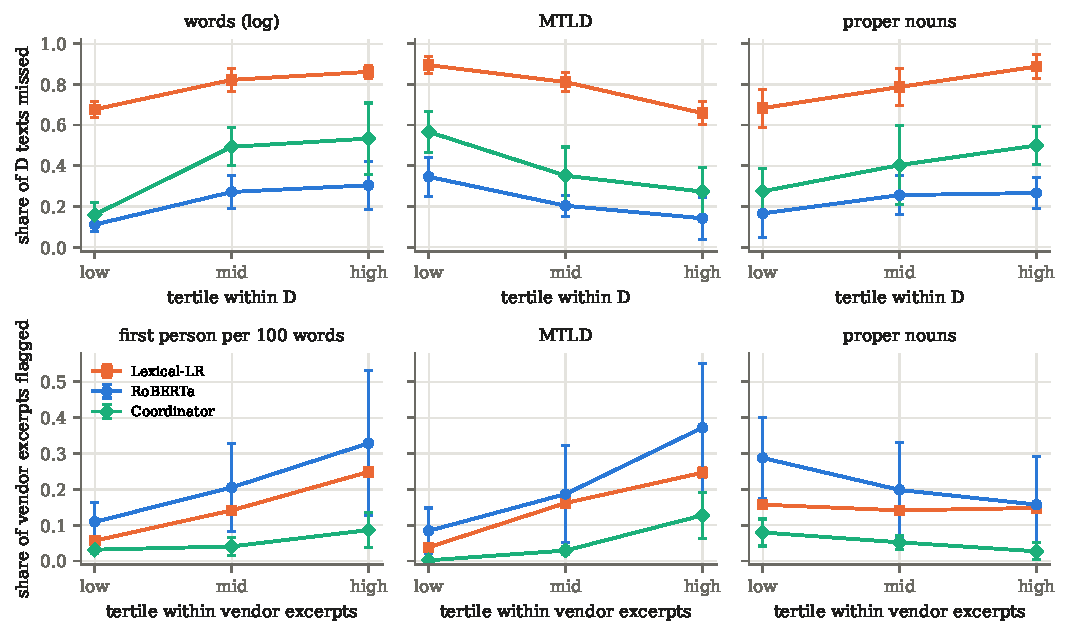
\includegraphics[width=0.92\textwidth]{error_by_bin.pdf}
\caption{Bir metin özelliğinin üçte birlik dilimlerine göre hata oranı (seed'ler üzerinden ortalama ve standart
sapma). Üst: tek üreticiyle eğitilen modellerin kaçırdığı D metinlerinin payı. Alt: ABC ile eğitilen modellerin
işaretlediği Microsoft ve Mandiant insan parçalarının payı.}
\label{fig:errbins}
\end{figure*}

\emph{D neden kaçıyor, E neden kaçmıyor.} D de E de büyük model ve ikisi de insan uzunluğunu tutturuyor. Aradaki
farkı uzunluk açıklamıyor. Tablo~\ref{tab:profile} anlatım kipini ve sözcük seçimini gösteriyor. Birinci şahıs
zamirleri D metinlerinin \ProfpctDFirst{} kadarında geçiyor. Bu, CISA parçalarındakinden (\ProfpctHumanFirst{}) bile
az. E metinlerinde oran \ProfpctEFirst{}, yani yerel üreticilerin aralığında (\ProfpctBFirst{} ile
\ProfpctCFirst{} arası). Lexical-LR'nin LLM yönünde ağırlık verdiği n-gram'lar 100 kelimede D'de \ProfDCuesLlm{},
E'de \ProfECuesLlm{}, yerel üreticilerde \ProfCCuesLlm{} ile \ProfACuesLlm{} arasında geçiyor (CISA:
\ProfHumanCuesLlm{}). D, insan yönlü n-gram'ları da bütün üreticilerden çok kullanıyor (\ProfDCuesHuman{}). E insan
uzunluğunda yazıyor ama küçük modellerin \emph{we} ve \emph{our} kullanımını ve tavsiye sözcüklerini koruyor. Bu
modellerle eğitilen bir dedektör onu tanıyor. D ise kişisiz yazıyor, tanımlayıcıları tekrarlıyor ve okura
seslenmiyor. Onu hâlâ LLM metni olarak ele veren şey sözcük çeşitliliği (medyan MTLD \MedMtldD{}, CISA'da
\MedMtldHuman{}). Sözcük çeşitliliği özelliklerinin D'yi tek başına tam stilometrik modelden daha iyi bulması ve
kaçanların en az çeşitli D metinleri olması bundan. Yazar şablonu da etkili. Lexical-LR olay müdahale raporu
şablonuyla yazılmış D metinlerinin \DmissIncidentLexlr{}, SOC bülteni şablonuyla yazılmış olanların
\DmissSocLexlr{} kadarını kaçırıyor; RoBERTa'da firma blogu şablonu \DmissBlogTrans{}, SOC bülteni şablonu
\DmissSocTrans{}. Örnekleme sıcaklığının etkisi yok (Lexical-LR'de 0.7 için \DmisstempLowLexlr{}, 1.0 için
\DmisstempHighLexlr{}).

\emph{Yanlış pozitifler.} CISA test parçalarında Lexical-LR hiç yanlış pozitif yapmıyor; RoBERTa bütün
çalıştırmalarda toplam \ErrtotalFpCisaTrans{} tane yapıyor: birinci şahısla yazılmış \ErrNFpCisaFirstPersonTrans{}
parça, \ErrNFpCisaProductVulnerabilityNoticeTrans{} ürün açığı bildirimi, az özel ad içeren
\ErrNFpCisaFewProperNounsTrans{} parça ve \ErrNFpCisaOtherTrans{} başka parça. Bu sayılar betimlemenin ötesine
geçmeye yetmiyor. Firma parçaları yeterli örnek veriyor (çalıştırma düzeyinde Lexical-LR'de
\ErrtotalFpVendorsLexlr{}, RoBERTa'da \ErrtotalFpVendorsTrans{}, Koordinatör'de \ErrtotalFpVendorsCoord{} yanlış
pozitif). Firma blogları kural olarak birinci şahısla yazıyor (Microsoft parçalarının \ProfpctMicrosoftFirst{},
Mandiant parçalarının \ProfpctMandiantFirst{} kadarı; CISA'da \ProfpctHumanFirst{}) ve birinci şahıs kategorisi
yanlış alarmlar içinde fazla temsil ediliyor (taban oranı \ErrbaseFpVendorsFirstPerson{} iken Lexical-LR'de
\ErrFpVendorsFirstPersonLexlr{}, RoBERTa'da \ErrFpVendorsFirstPersonTrans{}). Hangi parçaların işaretlendiğini
Tablo~\ref{tab:contrast} ve Şekil~\ref{fig:errbins}'in alt satırı gösteriyor. İşaretlenenlerin çeşitliliği daha
yüksek (MTLD için $\delta = \FpDeltaLexlrMtld$, $\FpDeltaTransMtld$ ve $\FpDeltaCoordMtld$), 100 kelimede birinci
şahıs kullanımı daha sık ($\FpDeltaLexlrFirstRate$ ve $\FpDeltaTransFirstRate$), LLM yönlü ipuçları daha çok
($\FpDeltaLexlrCuesLlm$ ve $\FpDeltaTransCuesLlm$); Lexical-LR ve Koordinatör'de ayrıca daha kısalar
($\FpDeltaLexlrNWords$ ve $\FpDeltaCoordNWords$). Derlem düzeyinde firmaları CISA'dan ayıran genel zamir oranı,
işaretlenen firma parçalarını geçenlerden ayırmıyor ($\FpDeltaLexlrPosPron$ ve $\FpDeltaTransPosPron$). Özel ad
oranı yalnızca RoBERTa'da ayırıyor ($\FpDeltaTransPosPropn$). Regresyonda bir standart sapma fazla birinci şahıs
kullanımı yanlış alarm olasılık oranını Lexical-LR'de \FpOrLexlrFirstRate{} (\%95 GA [\FpOrLoLexlrFirstRate{},
\FpOrHiLexlrFirstRate{}]), RoBERTa'da \FpOrTransFirstRate{} katına çıkarıyor. Bir standart sapma fazla MTLD ise
bu oranı sırasıyla \FpOrLexlrMtld{} ve \FpOrTransMtld{}, Koordinatör'de \FpOrCoordMtld{} katına çıkarıyor.

\emph{Örnekler.} Tablo~\ref{tab:examples} yüksek güvenle yapılmış altı hatayı gösteriyor. İlk D metni, olgularda
CertUtil yazan yerde \texttt{certutil.exe} yazdığı için tanımlayıcı eklemiş sayılıyor. Bu, kuralın ne kadar kaba
olduğunu gösteriyor. İkincisi SVR kısaltmasını ``Federal Security Service'' diye açıyor. Bu, başka bir Rus
kurumunun (FSB) adı ve bir üslup dedektörünün göremeyeceği bir içerik hatası. İki CISA yanlış pozitifinden biri
\emph{we} ile yazılmış ortak bir bildirim, diğeri az ad içeren bir anlatı özeti.

Birlikte bakıldığında iki hata türü birbirinin ayna görüntüsü. Kaçan LLM metinleri uzun, kişisiz, özel adı bol ve
sözcük çeşitliliği düşük metinler. Bu bir CISA parçasının profili. İşaretlenen insan metinleri daha kısa, birinci
şahısla yazılmış ve sözcük çeşitliliği yüksek metinler. Bu da eğitim üreticilerinin profili.

\section{Tartışma}\label{sec:discussion}
\subsection{Araştırma sorularının yanıtları}
\emph{S1, dilsel farklar.} LLM yazımı CTI'da sözcük çeşitliliği daha yüksek, bigram tekrarı daha az. Adı geçen
varlık daha az, okura verilen tavsiye daha çok. İnsan yazımı CTI tanımlayıcıları tekrarlıyor ve başka belgelere
atıf yapıyor. Bu, üretilen metnin belirli tokenların uzun kuyruğundan kaçındığını söyleyen GLTR gözlemiyle
örtüşüyor \cite{Gehrmann_2019}. Bu özelliklerin hepsi insan yazarlığının kendisini anlatmıyor. Birinci şahısla
anlatım CISA'yı hem küçük üreticilerden hem firma bloglarından ayırıyor, yani CISA'nın kurum üslubunu anlatıyor.
Daha genel olan fark sözcük çeşitliliği. Üç insan yayıncısı MTLD'de birbirine yakın, B'den E'ye üreticiler
bunların epey üstünde. Çeşitliliği en düşük üretici olan A ise firma bloglarıyla örtüşüyor
(Tablo~\ref{tab:profile}).

\emph{S2, baseline'lar ve transformer.} Aynı üreticide bir TF-IDF baseline'ı RoBERTa kadar iyi. Fark kaymada ortaya
çıkıyor. D'de RoBERTa'nın F1 değeri \FoneDTrans{}, Lexical-LR'ninki \FoneDLexLR{}; RoBERTa bunun için kurum
adlarına da muhtaç değil (adlar maskelenince \AblTransformerMaskedD{}). Önceden eğitilmiş temsiller, eğitim
üreticilerinin n-gram'larının ötesinde LLM yazısına özgü bir şeyler yakalıyor görünüyor; GPT-2 için kurulan
denetimli RoBERTa dedektörleri de böyleydi \cite{Solaiman_2019}. CTI verisi gerektirmeyen eğitimsiz dedektörler
burada metinleri eğitilmiş her modelden çok daha kötü sıralıyor. 2.7B'lik bir puanlama modeli ve 4 bitlik 7B
modellerle yazarlarının kurulumundan zayıflar. Üstelik RoBERTa'dan \RelFast{} ve \RelBino{} kat yavaşlar.

\emph{S3 ve S4, üretici üslubu ve üreticiler arası test.} Üç 7--8B yerel model arasında üreticiler arası F1, aynı
üreticideki değere yakın. Dedektörler yalnızca tek bir modelin üslubunu öğrenmiyor. Öğrendiklerinin bir kısmı ise
küçük modellerin CTI yazma biçimine özgü: kısa, birinci şahısla ve okura tavsiye vererek. Gemini daha uzun yazıyor
ama bu anlatımı koruyor ve yakalanıyor. gpt-oss-120b bu anlatımı bırakıyor ve sözcüksel modeller onu kaçırıyor;
AUC değerleri ise yüksek kalıyor. M4 ve RAID'de görülmemiş üreticilerin metninin insan yazımı sayılması da bu
örüntü \cite{Wang_2024,Dugan_2024}. Eşik sonuçlarımız sorunun kararda olduğunu gösteriyor, hata analizi de hangi
özelliklerin işe karıştığını söylüyor.

\emph{S5, önemli özellikler.} Stilometrik model çoğunlukla uzunluğa (en önemli özellik: \TopFeature{}) ve özel ad
oranına, sözcüksel model zamirlere, kaçamak kelimelere ve kurum adlarına bakıyor. Uzunluk ipucu büyük üreticilere
taşınmıyor. Sözcük çeşitliliği ipucu taşınıyor; D içinde kaçanlar da uzun, çeşitliliği düşük ve özel adı bol
metinler.

\emph{S6, konular ve saldırı türleri.} Yerel üreticiler arasında duyarlılık konuya bağlı değil. D'de zafiyet ve APT
raporları oltalama ve fidye yazılımı raporlarından daha çok kaçıyor (\TopicDVulnerability{} ve \TopicDApt{};
diğerlerinde \TopicDPhishing{} ve \TopicDRansomware{}). Olası bir neden, bu raporların olgularının çoğunlukla
aktör, ürün ve CVE adlarından oluşması ve bunun üretilen metnin özel ad oranını yükseltmesi. Konu etiketleri
anahtar kelime kurallarından geliyor ve çalıştırmalar arasındaki standart sapmalar büyük. Bunu bir eğilim olarak
okuyoruz.

\emph{S7, LLM teknolojisindeki değişim.} 2024 dönemi 7--8B modellerle eğitilen dedektörler en çok, daha büyük ve
yeni olan gpt-oss-120b'de kaybediyor. Aynı modellerin başka bir yöntemle ürettiği metinlerde, tek ajanlı yeniden
yazımda ve cümle düzeyinde karıştırmada da başarısız oluyorlar. Yeniden ifade iki dedektör grubunu farklı etkiledi.
Genel alan çalışmalarında olduğu gibi \cite{Krishna_2023,Sadasivan_2023} olabilirliğe dayalı iki dedektörün
duyarlılığını düşürdü, eğitilmiş olanlarınkini değiştirmedi. Akla yatkın bir açıklama, yeniden ifade için aynı
küçük talimat modellerini kullanmış olmamız. Yeniden ifade edilmiş metin o zaman aynı alışkanlıkları taşıyan başka
bir LLM metni oluyor ve bu tür metinlerle eğitilmiş bir sınıflandırıcı, token olasılıkları değişse de onu tanıyor.
RADAR'daki gibi tespitten kaçmak üzere eğitilmiş bir yeniden ifade modeli \cite{Hu_2023} daha zorlu bir sınama
olurdu.

\subsection{Sıralama ve karar}
Üretici ve yayıncı kaymasında denetimli dedektörlerin AUC değeri 1'e yakın kaldı. Değişen F1 ya da yanlış pozitif
oranıydı. Yeni metinle karşılaşan bir dedektör onu çoğunlukla hâlâ doğru sıralayabiliyor. Bozulan, eğitim
üreticilerine ve eğitim yayıncısına göre kurulmuş sınır. Dağılım içi doğrulama verisiyle kalibrasyon bunu
onarmıyor; Ovadia ve arkadaşlarının bulgusu da bu yönde \cite{Ovadia_2019}. Görülmemiş bir üretici için işe
yarayan iki onarım, insan skorlarından belirlenen eşik ve birkaç üreticiyle eğitim, sınırı insan metnine doğru
kaydırıyor ve ikisinin de bedeli modelin görmediği bir yayıncıda ödeniyor. Lexical-LR'nin Microsoft
parçalarındaki yanlış pozitif oranı, bir yerine üç üreticiyle eğitildiğinde \PoolfprOneMicrosoftLexlr{} değerinden
\PoolfprThreeMicrosoftLexlr{} değerine çıkıyor. İki kaymanın neden ters yönlere çektiğini hata analizi söylüyor.
Dedektörler CISA'yı küçük üreticilerden uzunluk, birinci şahısla anlatım ve sözcük çeşitliliği üzerinden ayırıyor.
İlk iki özellikte CISA'nın yakınında duran görülmemiş bir üretici kaçıyor. Son iki özellikte üreticilerin yakınında
duran görülmemiş bir yayıncı işaretleniyor. Bu özellikler üzerindeki tek bir sınır ikisine birden yetmiyor. Bu
bedeli ödetmeyen çare, birden fazla yayıncının insan metniydi. Bir firmanın parçalarını (\NExtChunksMicrosoft{}
veya \NExtChunksMandiant{} parça ve LLM sürümleri) eğitime eklemek, diğer firmadaki yanlış pozitif oranını birkaç
kat düşürdü.

\subsection{Ajanları birleştirmek ne zaman işe yarıyor}
Yığınlanmış Koordinatör, üyeleri farklı yerlerde yanıldığında işe yarıyor. Firma metinlerinde yanlış pozitif oranı
Lexical-LR ve RoBERTa'nınkinin yarısından az. En çok güvendiği üye başarısız olduğunda ise RoBERTa'nın gerisinde
kalıyor. Tek üreticiyle eğitimden sonra D'de olan bu. Ağırlıklar bütün üyelerin güvenilir göründüğü yerde
kuruluyor, bu yüzden yığın hangi üyenin yeni koşula taşınacağını bilemiyor. Ağırlıkları benzetilmiş bir kayma
altında öğrenmek kaybın bir kısmını geri getiriyor ve bu açıklamayı destekliyor. Uygulamada birleştirme kuralı
dışarıda tutulmuş üreticiler ve yayıncılar üzerinde seçilmeli. Buradaki LLM Yargıç gibi maliyet ekleyip sinyal
eklemeyen üyeler de çıkarılmalı.

\subsection{Bir CTI iş akışında kullanım}
Gelen raporların ön elemesinde bizim verimizdeki en iyi tek seçenek ince ayarlı bir kodlayıcı. GPU'da çıkarımı bir
TF-IDF modeli kadar ucuz, üretici kaymasında duyarlılığının çoğunu koruyor ve LLM ile yeniden ifadeye aldanmıyor.
Zayıf noktaları, yalnızca ilk 256 tokenı gördüğü kısmi üretim ve tanımadığı yayıncılardaki yanlış alarmlar. Bu
yüzden skoru bir raporu engellemek için değil analiste yönlendirmek için kullanılmalı, uzun raporlar pencere
pencere puanlanmalı ve her yeni rapor kaynağının insan metni, dedektöre o kaynakta güvenmeden önce eğitime
eklenmeli. Gerçek bir rapordan adları ve tanımlayıcıları kopyalayan sahte raporlar (tek ajanlı metinlerimiz gibi)
ve insan ile üretilmiş paragrafları karıştıran raporlar en büyük açık olarak kalıyor.

\section{Sınırlılıklar ve Geçerlilik Tehditleri}\label{sec:limits}
\subsection{Veri seti}
\emph{Eğitim yayıncısı.} Bütün eğitim metni CISA'dan geliyor. Bu yüzden eğitimde ``insan'' aynı zamanda ``bu
kurumun yazım üslubu'' anlamına geliyor. Microsoft ve Mandiant kümeleri bu yanlılığın ne kadar taşındığını ölçüyor,
ancak bunlar yayıncı etiketleri ve başlık kurallarıyla seçilmiş firma blogları ve \NExtSourcesMicrosoft{} artı
\NExtSourcesMandiant{} kaynak, firma yazımının küçük bir örneği. STIX nesneleri, analist yazışmaları veya İngilizce
olmayan raporlar gibi başka CTI biçimleri kapsanmıyor. \emph{Boyut.} \NSources{} CISA kaynağı seed başına yaklaşık
40 kaynaklık test kümeleri veriyor. Ortalamaların yanında kaynak düzeyindeki aralıkları da bu yüzden veriyoruz.
Bazı alt kümeler çok daha küçük: tek ajanlı test metinleri, uzunluğu eşleştirilmiş alt kümeler ve taban oranı düşük
hata kategorileri. \emph{Tarihler.} İnsan yazarlığı 30 Kasım 2022 veya öncesindeki yayın tarihlerine dayanıyor.
CISA sayfaları revizyon tarihini gösteriyor, Microsoft üst verileri bir site taşımasıyla değişmiş ve Mandiant
yazıları yeni bir sunucuya taşınmış. Bu yüzden belgeleri bildirim kodlarına, URL tarihlerine ve görünür yazar
satırlarına göre tarihliyor ve sonraki güncellemeleri duyuran paragrafları siliyoruz. Tarih sınırından sonra böyle
bir not olmadan değiştirilmiş bir paragraf fark edilmezdi. \emph{Dışarıda kalan sayfalar.} Yerel antivirüs gömülü
zararlı yazılım örneklerini işaretlediği için \NBlocked{} CISA analiz raporu okunamadı.

\subsection{Üretim}
\emph{Üretici kapsamı.} Üç eğitim üreticisi 2024'ten 7--8B boyutunda açık modeller. D ve E yalnızca çok ajanlı
koşulda ve kota kısıtlamasından önce üretilenler dışında yalnızca test parçaları için var. Bu yüzden daha büyük
modellerle eğitim yapamıyor, tek ajanlı yeniden yazımı ve dış yayıncıları bu modellerle sınayamıyoruz. D ile E
arasındaki karşıtlık her türden tek bir modele dayanıyor. \emph{Tek hat.} Bütün LLM metinleri tek bir prompt
kümesinden ve tek bir Analist'ten geliyor. Tek ajan ve prompt stratejisi koşulları başka bir yöntemin sonuçları
değiştirdiğini gösteriyor. \emph{Olgu kayması.} Üreticiler bazen olguları değiştirdi veya ekledi. Bu metinler
ayıklanmadı ve alan bilgisi olan bir okur bazılarını içerikten fark edebilir. Eklenen tanımlayıcılar için
kullandığımız ölçü bir örüntü eşlemesi. Uydurulmuş anlatıyı yakalamıyor. \emph{İnsan tarafından düzenlenmiş metin
yok.} Bir saldırgan bir LLM taslağını bir insana düzelttirebilir. Bu tür metinleri toplamadık ve başka bir LLM ile
taklit etmemeyi seçtik, çünkü bu yine LLM yeniden yazımını ölçmek olurdu. Cümle düzeyindeki karışımlar, insan ve
makine paragraflarından derlenmiş bir rapora yaklaşıyor, makine metninin insan tarafından düzenlenmesine değil;
LLM etiketleri de bir kabul.

\subsection{Dedektörler ve analiz}
\emph{Model seçimi.} RoBERTa tek ince ayarlı kodlayıcı, Gemma~2~9B tek yargıç. Hiperparametre araması yapılmadı.
Binoculars 4 bit hassasiyetle ve skorlarını kaydıran kırpılmış bir gözlemci dağılımıyla, Fast-DetectGPT tek bir
2.7B modelle çalıştı. İkisi de yazarlarının en güçlü ayarlarından küçük; Ghostbuster çalıştırılamadı.
\emph{Kalibrasyon verisi.} Kalibratörler ve eşikler seed başına 20 civarında kaynaktan oluşan doğrulama
kümelerinden geliyor. Kırk kadar insan skorunun 99. yüzdeliği en büyük skora yakın; \%1 kuralı CISA test metninde
\ThrInLexlrHumoneFpr{} ile \ThrInTransHumoneFpr{} arasında yanlış pozitif oranı veriyor. \emph{Hata analizi.}
Kategoriler kural tabanlı, tek bir yazar tarafından tanımlanmış ve ikinci bir işaretleyiciyle kontrol edilmemiş.
Özellik karşılaştırmaları ve regresyonlar gözlemsel: hangi metinlerin yanlış sınıflandırıldığını gösteriyorlar,
bir özelliği değiştirmenin kararı değiştireceğini kanıtlamıyorlar. İpucu listeleri A ile eğitilen tek bir modelden
geliyor. \emph{İstatistik.} Bootstrap aralıkları test kaynaklarını yeniden örnekliyor, ancak üç seed'i ve eğitim
üreticilerini veri olarak alıyor. Farklı bir üretici seçiminin varyansını yansıtmıyor. $p$ değerleri $2/2001$
değerinden küçük olamıyor.

\section{Sonuç}
İnsan ve LLM yazımı CTI ölçülebilir biçimde farklı ve üretici biliniyorsa bunları ayırmaya bir TF-IDF modeli
yetiyor. Zorluk, dedektörün görmediği metinle başlıyor. Beş üreticinin aynı çıkarılmış olgulardan yazdığı
derlemimizde dedektörler bu metinleri doğru sıralamayı sürdürdü, kararı ise kaybetti: kişisiz yazan büyük ve
görülmemiş bir üretici eşiğin altında, birinci şahısla yazılmış firma blogları eşiğin üstünde skor aldı. Eğitim
üreticilerini havuzlamak ya da eşiği insan skorlarından belirlemek ilk hatayı onardı, ikincisini büyüttü. Doğrulama
verisiyle kalibrasyon ikisini de onarmadı. Bu bedeli ödetmeyen tek çare, eğitime ikinci bir yayıncının insan metnini
katmaktı. Dedektör ajanlarının yığınlanmış birleşimi firma metinlerinde maliyetine değdi, en çok güvendiği üyenin
çöktüğü yerde RoBERTa'nın gerisinde kaldı. Bir LLM metnini bir LLM ile yeniden yazmak onu eğitilmiş dedektörlerden
gizlemedi. Kaynağı okuyarak yeniden yazmak ve insan cümleleriyle üretilmiş cümleleri karıştırmak ise gizledi.
Çalışma, eğitim için tek bir devlet yayıncısıyla, üç küçük eğitim üreticisiyle ve tek bir üretim hattıyla sınırlı.
İnsan tarafından düzenlenmiş LLM taslakları, daha büyük eğitim üreticileri ve uzun raporların pencere pencere
puanlanması sonraki adımlar.

\section*{Yeniden Üretilebilirlik}
Kod, yapılandırma dosyaları, CISA derlemi, üretilen bütün metinler ve ajan mesajları, tahminler ve sonuç tabloları
proje reposunda yer alıyor.\footnote{\url{https://github.com/FurkanDevelops/llm-cti-detection}} Her aşama tek bir
komutla çalışıyor, \texttt{python -m src.cli <aşama> --config <dosya>}; \texttt{experiments/run\_all.sh} hepsini
sırayla çalıştırıyor. Model adları, promptlar, örnekleme sıcaklıkları, seed'ler ve dedektör ayarları
\texttt{configs/} içinde. Paket sürümleri \texttt{requirements.txt} içinde sabitlenmiş. Bu makaledeki her sayı
rapor aşaması tarafından bir makro dosyasına yazılıyor. Böylece metin sonuçlardan kopamıyor. Microsoft ve Mandiant
parçaları toplama betiği tarafından listelenen URL'lerden yeniden oluşturuluyor ve kayıtlı özetlerle (hash)
karşılaştırılıyor. API üretimleri (D, E) birebir tekrarlanamadığı için çıktıları saklanıyor.

\bibliographystyle{IEEEtran}
\bibliography{../refs}

\end{document}
